\documentclass[a4paper]{book}
\usepackage{makeidx}
\usepackage{graphicx}
\usepackage{multicol}
\usepackage{float}
\usepackage{listings}
\usepackage{color}
\usepackage{ifthen}
\usepackage[table]{xcolor}
\usepackage{textcomp}
\usepackage{alltt}
\usepackage[utf8]{inputenc}
\usepackage{mathptmx}
\usepackage[scaled=.90]{helvet}
\usepackage{courier}
\usepackage{doxygen}
\lstset{language=C++,inputencoding=utf8,basicstyle=\footnotesize,breaklines=true,breakatwhitespace=true,tabsize=8,numbers=left }
\makeindex
\setcounter{tocdepth}{3}
\renewcommand{\footrulewidth}{0.4pt}
\begin{document}
\begin{titlepage}
\vspace*{7cm}
\begin{center}
{\Large Robot Simulation }\\
\vspace*{1cm}
{\large Generated by Doxygen 1.7.3}\\
\vspace*{0.5cm}
{\small Mon Mar 28 2011 23:56:56}\\
\end{center}
\end{titlepage}
\clearemptydoublepage
\pagenumbering{roman}
\tableofcontents
\clearemptydoublepage
\pagenumbering{arabic}
\chapter{Namespace Index}
\section{Packages}
Here are the packages with brief descriptions (if available):\begin{DoxyCompactList}
\item\contentsline{section}{{\bf attempt\_\-7} }{\pageref{namespaceattempt__7}}{}
\item\contentsline{section}{{\bf Attempt\_\-7} }{\pageref{namespace_attempt__7}}{}
\end{DoxyCompactList}

\chapter{Class Index}
\section{Class List}
Here are the classes, structs, unions and interfaces with brief descriptions:\begin{DoxyCompactList}
\item\contentsline{section}{{\bf Attempt\_\-7.Camera} (Represents the camera object/class that contains all the information needed about position and target for rendering )}{\pageref{class_attempt__7_1_1_camera}}{}
\item\contentsline{section}{{\bf Attempt\_\-7.DrawImageAnalysis} (This is a game component that implements IUpdateable. Draws the image analysis information )}{\pageref{class_attempt__7_1_1_draw_image_analysis}}{}
\item\contentsline{section}{{\bf Attempt\_\-7.ImageAnalysis} (It was easier to redure 640$\ast$480 small triangles and view then from a distance than to put a texture on the GPU So there is a camera to view the triangels. The class only analzes a small fraction of the pixels each time through the game loop inorder to keep the speed high. Many of the methods have loops that cause them to only look at every X pixel each time through and then the next time through a different set. Basically it functions like a giant double \char`\"{}for\char`\"{} loop )}{\pageref{class_attempt__7_1_1_image_analysis}}{}
\item\contentsline{section}{{\bf Attempt\_\-7.Robot} }{\pageref{class_attempt__7_1_1_robot}}{}
\item\contentsline{section}{{\bf Attempt\_\-7.SimulationMain} (This is the main type for the Simulation )}{\pageref{class_attempt__7_1_1_simulation_main}}{}
\item\contentsline{section}{{\bf attempt\_\-7.UserControl1} }{\pageref{classattempt__7_1_1_user_control1}}{}
\end{DoxyCompactList}

\chapter{File Index}
\section{File List}
Here is a list of all files with brief descriptions:\begin{DoxyCompactList}
\item\contentsline{section}{C:/Users/Anthony/Dropbox/Senior Project/attempt 7/attempt 7/attempt 7/{\bf Camera.cs} }{\pageref{_camera_8cs}}{}
\item\contentsline{section}{C:/Users/Anthony/Dropbox/Senior Project/attempt 7/attempt 7/attempt 7/{\bf DrawImageAnalysis.cs} }{\pageref{_draw_image_analysis_8cs}}{}
\item\contentsline{section}{C:/Users/Anthony/Dropbox/Senior Project/attempt 7/attempt 7/attempt 7/{\bf DrawImageAnalysis2.cs} }{\pageref{_draw_image_analysis2_8cs}}{}
\item\contentsline{section}{C:/Users/Anthony/Dropbox/Senior Project/attempt 7/attempt 7/attempt 7/{\bf ImageAnalysis.cs} }{\pageref{_image_analysis_8cs}}{}
\item\contentsline{section}{C:/Users/Anthony/Dropbox/Senior Project/attempt 7/attempt 7/attempt 7/{\bf ImageAnalysis2.cs} }{\pageref{_image_analysis2_8cs}}{}
\item\contentsline{section}{C:/Users/Anthony/Dropbox/Senior Project/attempt 7/attempt 7/attempt 7/{\bf Program.cs} }{\pageref{_program_8cs}}{}
\item\contentsline{section}{C:/Users/Anthony/Dropbox/Senior Project/attempt 7/attempt 7/attempt 7/{\bf Robot.cs} }{\pageref{_robot_8cs}}{}
\item\contentsline{section}{C:/Users/Anthony/Dropbox/Senior Project/attempt 7/attempt 7/attempt 7/{\bf SimulationMain.cs} }{\pageref{_simulation_main_8cs}}{}
\item\contentsline{section}{C:/Users/Anthony/Dropbox/Senior Project/attempt 7/attempt 7/attempt 7/{\bf UserControl1.cs} }{\pageref{_user_control1_8cs}}{}
\item\contentsline{section}{C:/Users/Anthony/Dropbox/Senior Project/attempt 7/attempt 7/attempt 7/{\bf UserControl1.Designer.cs} }{\pageref{_user_control1_8_designer_8cs}}{}
\item\contentsline{section}{C:/Users/Anthony/Dropbox/Senior Project/attempt 7/attempt 7/attempt 7/Properties/{\bf AssemblyInfo.cs} }{\pageref{_assembly_info_8cs}}{}
\end{DoxyCompactList}

\chapter{Namespace Documentation}
\section{Package attempt\_\-7}
\label{namespaceattempt__7}\index{attempt\_\-7@{attempt\_\-7}}
\subsection*{Classes}
\begin{DoxyCompactItemize}
\item 
class {\bf UserControl1}
\end{DoxyCompactItemize}

\section{Package Attempt\_\-7}
\label{namespace_attempt__7}\index{Attempt\_\-7@{Attempt\_\-7}}
\subsection*{Classes}
\begin{DoxyCompactItemize}
\item 
class {\bf Camera}
\begin{DoxyCompactList}\small\item\em Represents the camera object/class that contains all the information needed about position and target for rendering. \item\end{DoxyCompactList}\item 
class {\bf DrawImageAnalysis}
\begin{DoxyCompactList}\small\item\em This is a game component that implements IUpdateable. Draws the image analysis information. \item\end{DoxyCompactList}\item 
class {\bf ImageAnalysis}
\begin{DoxyCompactList}\small\item\em It was easier to redure 640$\ast$480 small triangles and view then from a distance than to put a texture on the GPU So there is a camera to view the triangels. The class only analzes a small fraction of the pixels each time through the game loop inorder to keep the speed high. Many of the methods have loops that cause them to only look at every X pixel each time through and then the next time through a different set. Basically it functions like a giant double \char`\"{}for\char`\"{} loop. \item\end{DoxyCompactList}\item 
class {\bf Robot}
\item 
class {\bf SimulationMain}
\begin{DoxyCompactList}\small\item\em This is the main type for the Simulation. \item\end{DoxyCompactList}\end{DoxyCompactItemize}

\chapter{Class Documentation}
\section{Attempt\_\-7.Camera Class Reference}
\label{class_attempt__7_1_1_camera}\index{Attempt\_\-7::Camera@{Attempt\_\-7::Camera}}


Represents the camera object/class that contains all the information needed about position and target for rendering.  


\subsection*{Public Member Functions}
\begin{DoxyCompactItemize}
\item 
{\bf Camera} (Game game, Vector3 pos, Vector3 {\bf target}, Vector3 up, bool {\bf isMouseDependent})
\begin{DoxyCompactList}\small\item\em Initializes a new instance of the \doxyref{Camera}{p.}{class_attempt__7_1_1_camera} class. \item\end{DoxyCompactList}\item 
override void {\bf Initialize} ()
\begin{DoxyCompactList}\small\item\em Initializes the camera. \item\end{DoxyCompactList}\item 
override void {\bf Update} (GameTime gameTime)
\begin{DoxyCompactList}\small\item\em Updates the camera's view. If the camera is mouse dependent than Update gets the position of the mouse and keyboard inorder to update the camera position. \item\end{DoxyCompactList}\item 
Vector3 {\bf GetCameraPosition} ()
\begin{DoxyCompactList}\small\item\em Returns the current camera position in 3D space. \item\end{DoxyCompactList}\item 
void {\bf SetCameraPositionAndTarget} (Vector3 pos, Vector3 {\bf target})
\begin{DoxyCompactList}\small\item\em Sets the camera position and target point to a specific position. \item\end{DoxyCompactList}\end{DoxyCompactItemize}
\subsection*{Public Attributes}
\begin{DoxyCompactItemize}
\item 
Matrix {\bf View}
\begin{DoxyCompactList}\small\item\em Matrix representation of the view determined by the position, target, and updirection. \item\end{DoxyCompactList}\item 
Matrix {\bf Projection}
\begin{DoxyCompactList}\small\item\em Matrix representation of the view determined by the angle of the field of view (Pi/4), aspectRatio, nearest plane visible (1), and farthest plane visible (1200) \item\end{DoxyCompactList}\item 
Matrix {\bf World}
\begin{DoxyCompactList}\small\item\em Matrix representing how the real world cordinates differ from that of the rendering by the camera. \item\end{DoxyCompactList}\end{DoxyCompactItemize}
\subsection*{Private Member Functions}
\begin{DoxyCompactItemize}
\item 
void {\bf UpdateMouse} ()
\begin{DoxyCompactList}\small\item\em Updates the position of the camera based on the mouse's position. The Mouse origin (0,0) is the top left corner of the simulation Window. \item\end{DoxyCompactList}\item 
void {\bf UpdateKeyBoard} ()
\begin{DoxyCompactList}\small\item\em Checks to see if the Arrow keys are pressed. Moves the camera position and target based on the arrow keys. \item\end{DoxyCompactList}\end{DoxyCompactItemize}
\subsection*{Private Attributes}
\begin{DoxyCompactItemize}
\item 
Vector3 {\bf cameraPosition} = Vector3.Zero
\begin{DoxyCompactList}\small\item\em The position of the camera. Defualt = 0,0,0. \item\end{DoxyCompactList}\item 
Vector3 {\bf target} = Vector3.Zero
\begin{DoxyCompactList}\small\item\em Target of the camera = a point in 3D space that the camera is pointed at. \item\end{DoxyCompactList}\item 
Vector3 {\bf updirection}
\begin{DoxyCompactList}\small\item\em The 3D vector that defines which direction is up for the camera. \item\end{DoxyCompactList}\item 
Vector3 {\bf mouseOffset}
\begin{DoxyCompactList}\small\item\em If the camera is mouse controlled, how much should the mouse cordinates differ from 3D cordinates in space. How much should they be translated in 3D space. \item\end{DoxyCompactList}\item 
bool {\bf isMouseDependent}
\begin{DoxyCompactList}\small\item\em If the camera is mouse dependent than the position of the mouse determines the position of the camera in 3D space. \item\end{DoxyCompactList}\end{DoxyCompactItemize}


\subsection{Detailed Description}
Represents the camera object/class that contains all the information needed about position and target for rendering. 

Definition at line 25 of file Camera.cs.



\subsection{Constructor \& Destructor Documentation}
\index{Attempt\_\-7::Camera@{Attempt\_\-7::Camera}!Camera@{Camera}}
\index{Camera@{Camera}!Attempt_7::Camera@{Attempt\_\-7::Camera}}
\subsubsection[{Camera}]{\setlength{\rightskip}{0pt plus 5cm}Attempt\_\-7.Camera.Camera (
\begin{DoxyParamCaption}
\item[{Game}]{game, }
\item[{Vector3}]{pos, }
\item[{Vector3}]{target, }
\item[{Vector3}]{up, }
\item[{bool}]{isMouseDependent}
\end{DoxyParamCaption}
)}\label{class_attempt__7_1_1_camera_a00dbb72fcaebdd53a8206071f2da796b}


Initializes a new instance of the \doxyref{Camera}{p.}{class_attempt__7_1_1_camera} class. 


\begin{DoxyParams}{Parameters}
{\em game} & The game object of the simulation\\
\hline
{\em pos} & The start position of the camera in 3D space\\
\hline
{\em target} & A point in 3D space that the camera will point at. \\
\hline
{\em up} & The 3D vector that determines which direction is up for the camera\\
\hline
{\em isMouseDependent} & Sets the camera's position based on the mouse if true\\
\hline
\end{DoxyParams}


Definition at line 75 of file Camera.cs.


\begin{DoxyCode}
            : base(game)
        {
            this.cameraPosition = pos;
            this.target = target;
            this.updirection = up;
            this.View = Matrix.CreateLookAt(pos, target, up);
            this.Projection = Matrix.CreatePerspectiveFieldOfView(MathHelper.PiOv
      er4, (float)Game.Window.ClientBounds.Width / (float)Game.Window.ClientBounds.Heig
      ht, 1, 1200);
            this.isMouseDependent = isMouseDependent;
            this.World = Matrix.Identity;
            this.mouseOffset = pos;
        }
\end{DoxyCode}


\subsection{Member Function Documentation}
\index{Attempt\_\-7::Camera@{Attempt\_\-7::Camera}!GetCameraPosition@{GetCameraPosition}}
\index{GetCameraPosition@{GetCameraPosition}!Attempt_7::Camera@{Attempt\_\-7::Camera}}
\subsubsection[{GetCameraPosition}]{\setlength{\rightskip}{0pt plus 5cm}Vector3 Attempt\_\-7.Camera.GetCameraPosition (
\begin{DoxyParamCaption}
{}
\end{DoxyParamCaption}
)}\label{class_attempt__7_1_1_camera_a0574b1158af6b8e99f5d2b21fbc3c7a8}


Returns the current camera position in 3D space. 

\begin{DoxyReturn}{Returns}
The camera position
\end{DoxyReturn}


Definition at line 117 of file Camera.cs.


\begin{DoxyCode}
        {
            return this.cameraPosition;
        }
\end{DoxyCode}
\index{Attempt\_\-7::Camera@{Attempt\_\-7::Camera}!Initialize@{Initialize}}
\index{Initialize@{Initialize}!Attempt_7::Camera@{Attempt\_\-7::Camera}}
\subsubsection[{Initialize}]{\setlength{\rightskip}{0pt plus 5cm}override void Attempt\_\-7.Camera.Initialize (
\begin{DoxyParamCaption}
{}
\end{DoxyParamCaption}
)}\label{class_attempt__7_1_1_camera_a3007d7c03912d7ff6f6f19e90a3575c2}


Initializes the camera. 



Definition at line 91 of file Camera.cs.


\begin{DoxyCode}
        {
            base.Initialize();
        }
\end{DoxyCode}
\index{Attempt\_\-7::Camera@{Attempt\_\-7::Camera}!SetCameraPositionAndTarget@{SetCameraPositionAndTarget}}
\index{SetCameraPositionAndTarget@{SetCameraPositionAndTarget}!Attempt_7::Camera@{Attempt\_\-7::Camera}}
\subsubsection[{SetCameraPositionAndTarget}]{\setlength{\rightskip}{0pt plus 5cm}void Attempt\_\-7.Camera.SetCameraPositionAndTarget (
\begin{DoxyParamCaption}
\item[{Vector3}]{pos, }
\item[{Vector3}]{target}
\end{DoxyParamCaption}
)}\label{class_attempt__7_1_1_camera_a950a4219356e02b8b8eddf506c03743f}


Sets the camera position and target point to a specific position. 


\begin{DoxyParams}{Parameters}
{\em pos} & The new position of the camera in 3D space\\
\hline
{\em target} & The new target point of the camera in 3D space\\
\hline
\end{DoxyParams}


Definition at line 127 of file Camera.cs.


\begin{DoxyCode}
        {
            this.cameraPosition = pos;
            this.target = target;
        }
\end{DoxyCode}


Here is the caller graph for this function:\nopagebreak
\begin{figure}[H]
\begin{center}
\leavevmode
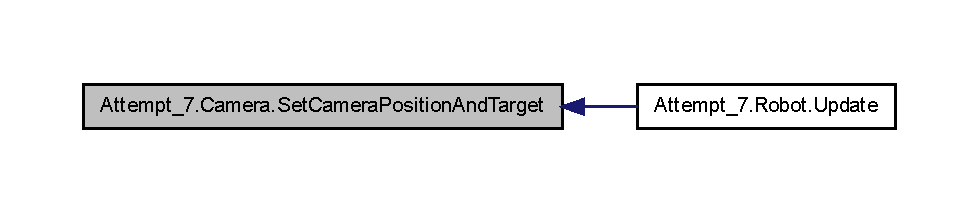
\includegraphics[width=400pt]{class_attempt__7_1_1_camera_a950a4219356e02b8b8eddf506c03743f_icgraph}
\end{center}
\end{figure}


\index{Attempt\_\-7::Camera@{Attempt\_\-7::Camera}!Update@{Update}}
\index{Update@{Update}!Attempt_7::Camera@{Attempt\_\-7::Camera}}
\subsubsection[{Update}]{\setlength{\rightskip}{0pt plus 5cm}override void Attempt\_\-7.Camera.Update (
\begin{DoxyParamCaption}
\item[{GameTime}]{gameTime}
\end{DoxyParamCaption}
)}\label{class_attempt__7_1_1_camera_a0090d02f2acd45b0088ecd0123be57ef}


Updates the camera's view. If the camera is mouse dependent than Update gets the position of the mouse and keyboard inorder to update the camera position. 


\begin{DoxyParams}{Parameters}
{\em gameTime} & Clock Information\\
\hline
\end{DoxyParams}


Definition at line 100 of file Camera.cs.


\begin{DoxyCode}
        {
            if (this.isMouseDependent == true)
            {
                this.UpdateMouse();
                this.UpdateKeyBoard();
            }

            this.View = Matrix.CreateLookAt(this.cameraPosition, this.target, thi
      s.updirection); // Update the veiw. 
          
            base.Update(gameTime);
        }
\end{DoxyCode}


Here is the call graph for this function:\nopagebreak
\begin{figure}[H]
\begin{center}
\leavevmode
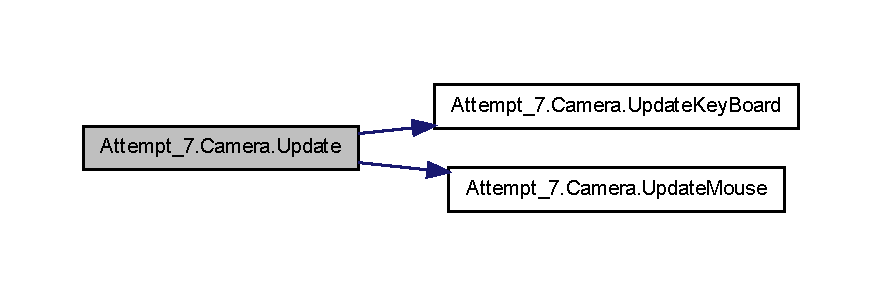
\includegraphics[width=400pt]{class_attempt__7_1_1_camera_a0090d02f2acd45b0088ecd0123be57ef_cgraph}
\end{center}
\end{figure}




Here is the caller graph for this function:\nopagebreak
\begin{figure}[H]
\begin{center}
\leavevmode
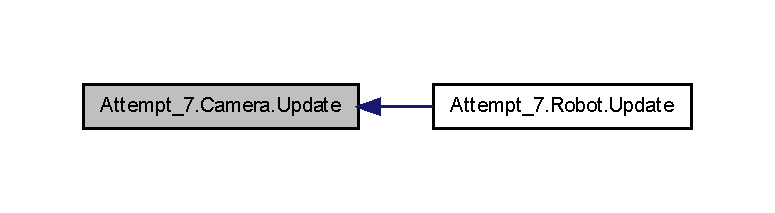
\includegraphics[width=372pt]{class_attempt__7_1_1_camera_a0090d02f2acd45b0088ecd0123be57ef_icgraph}
\end{center}
\end{figure}


\index{Attempt\_\-7::Camera@{Attempt\_\-7::Camera}!UpdateKeyBoard@{UpdateKeyBoard}}
\index{UpdateKeyBoard@{UpdateKeyBoard}!Attempt_7::Camera@{Attempt\_\-7::Camera}}
\subsubsection[{UpdateKeyBoard}]{\setlength{\rightskip}{0pt plus 5cm}void Attempt\_\-7.Camera.UpdateKeyBoard (
\begin{DoxyParamCaption}
{}
\end{DoxyParamCaption}
)\hspace{0.3cm}{\ttfamily  [private]}}\label{class_attempt__7_1_1_camera_a26c1b12ed3fea81c3bed64f0389cc9d1}


Checks to see if the Arrow keys are pressed. Moves the camera position and target based on the arrow keys. 



Definition at line 154 of file Camera.cs.


\begin{DoxyCode}
        {
            KeyboardState keyboardState = Keyboard.GetState();
            if (keyboardState.IsKeyDown(Keys.Left))
            {
                this.target += Vector3.Left / 3;
                this.mouseOffset += Vector3.Left / 3;
            }

            if (keyboardState.IsKeyDown(Keys.Right))
            {
                this.target += Vector3.Right / 3;
                this.mouseOffset += Vector3.Right / 3;
            }

            if (keyboardState.IsKeyDown(Keys.Up))
            {
                this.target += Vector3.Up / 3;
                this.mouseOffset += Vector3.Up / 3;
            }

            if (keyboardState.IsKeyDown(Keys.Down))
            {
                this.target += Vector3.Down / 3;
                this.mouseOffset += Vector3.Down / 3;
            }
        }
\end{DoxyCode}


Here is the caller graph for this function:\nopagebreak
\begin{figure}[H]
\begin{center}
\leavevmode
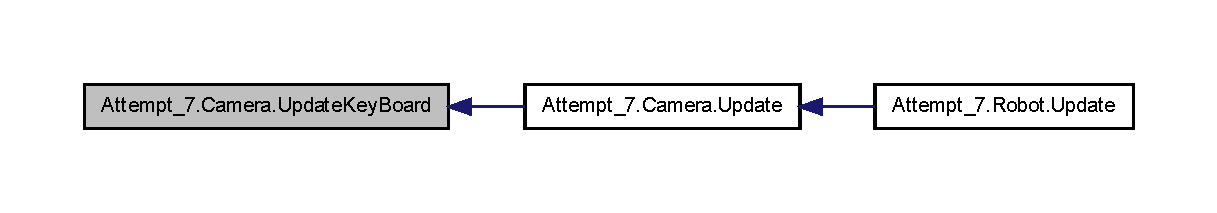
\includegraphics[width=400pt]{class_attempt__7_1_1_camera_a26c1b12ed3fea81c3bed64f0389cc9d1_icgraph}
\end{center}
\end{figure}


\index{Attempt\_\-7::Camera@{Attempt\_\-7::Camera}!UpdateMouse@{UpdateMouse}}
\index{UpdateMouse@{UpdateMouse}!Attempt_7::Camera@{Attempt\_\-7::Camera}}
\subsubsection[{UpdateMouse}]{\setlength{\rightskip}{0pt plus 5cm}void Attempt\_\-7.Camera.UpdateMouse (
\begin{DoxyParamCaption}
{}
\end{DoxyParamCaption}
)\hspace{0.3cm}{\ttfamily  [private]}}\label{class_attempt__7_1_1_camera_ac8b5117b5378692c67dada10a2707ad9}


Updates the position of the camera based on the mouse's position. The Mouse origin (0,0) is the top left corner of the simulation Window. 



Definition at line 136 of file Camera.cs.


\begin{DoxyCode}
        {
            Vector3 mouseVector = Vector3.Zero;
            MouseState mouse = Mouse.GetState(); // Create a mouse state object

            mouseVector.X = mouse.X; // Moving the mosue left and right is the ca
      mera position x axis
            mouseVector.Y = mouse.Y; // Moving the mouse up and down is the camer
      a position y axis
            mouseVector.Z = (int)mouse.ScrollWheelValue; // Mouse scroll wheel to
      tal is the camera position z axis

            this.cameraPosition.X = mouseVector.X / 10;
            this.cameraPosition.Y = mouseVector.Y / 10;
            this.cameraPosition.Z = mouseVector.Z / 60;
            this.cameraPosition += this.mouseOffset;
        }
\end{DoxyCode}


Here is the caller graph for this function:\nopagebreak
\begin{figure}[H]
\begin{center}
\leavevmode
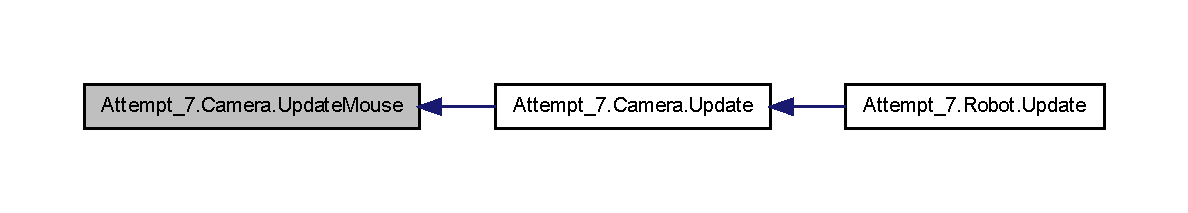
\includegraphics[width=400pt]{class_attempt__7_1_1_camera_ac8b5117b5378692c67dada10a2707ad9_icgraph}
\end{center}
\end{figure}




\subsection{Member Data Documentation}
\index{Attempt\_\-7::Camera@{Attempt\_\-7::Camera}!cameraPosition@{cameraPosition}}
\index{cameraPosition@{cameraPosition}!Attempt_7::Camera@{Attempt\_\-7::Camera}}
\subsubsection[{cameraPosition}]{\setlength{\rightskip}{0pt plus 5cm}Vector3 {\bf Attempt\_\-7.Camera.cameraPosition} = Vector3.Zero\hspace{0.3cm}{\ttfamily  [private]}}\label{class_attempt__7_1_1_camera_ac5ff73c169cf1db99dc2c95e4a2d8464}


The position of the camera. Defualt = 0,0,0. 



Definition at line 45 of file Camera.cs.

\index{Attempt\_\-7::Camera@{Attempt\_\-7::Camera}!isMouseDependent@{isMouseDependent}}
\index{isMouseDependent@{isMouseDependent}!Attempt_7::Camera@{Attempt\_\-7::Camera}}
\subsubsection[{isMouseDependent}]{\setlength{\rightskip}{0pt plus 5cm}bool {\bf Attempt\_\-7.Camera.isMouseDependent}\hspace{0.3cm}{\ttfamily  [private]}}\label{class_attempt__7_1_1_camera_afa316d43d2017c000a0650706956d08b}


If the camera is mouse dependent than the position of the mouse determines the position of the camera in 3D space. 



Definition at line 65 of file Camera.cs.

\index{Attempt\_\-7::Camera@{Attempt\_\-7::Camera}!mouseOffset@{mouseOffset}}
\index{mouseOffset@{mouseOffset}!Attempt_7::Camera@{Attempt\_\-7::Camera}}
\subsubsection[{mouseOffset}]{\setlength{\rightskip}{0pt plus 5cm}Vector3 {\bf Attempt\_\-7.Camera.mouseOffset}\hspace{0.3cm}{\ttfamily  [private]}}\label{class_attempt__7_1_1_camera_a2595f02eb31f80ea60343ba98fdbc5ff}


If the camera is mouse controlled, how much should the mouse cordinates differ from 3D cordinates in space. How much should they be translated in 3D space. 



Definition at line 60 of file Camera.cs.

\index{Attempt\_\-7::Camera@{Attempt\_\-7::Camera}!Projection@{Projection}}
\index{Projection@{Projection}!Attempt_7::Camera@{Attempt\_\-7::Camera}}
\subsubsection[{Projection}]{\setlength{\rightskip}{0pt plus 5cm}Matrix {\bf Attempt\_\-7.Camera.Projection}}\label{class_attempt__7_1_1_camera_afad745cd526a8c616843da8464a4d256}


Matrix representation of the view determined by the angle of the field of view (Pi/4), aspectRatio, nearest plane visible (1), and farthest plane visible (1200) 



Definition at line 35 of file Camera.cs.

\index{Attempt\_\-7::Camera@{Attempt\_\-7::Camera}!target@{target}}
\index{target@{target}!Attempt_7::Camera@{Attempt\_\-7::Camera}}
\subsubsection[{target}]{\setlength{\rightskip}{0pt plus 5cm}Vector3 {\bf Attempt\_\-7.Camera.target} = Vector3.Zero\hspace{0.3cm}{\ttfamily  [private]}}\label{class_attempt__7_1_1_camera_a2ab493dc1de314f87a198146bf87db54}


Target of the camera = a point in 3D space that the camera is pointed at. 



Definition at line 50 of file Camera.cs.

\index{Attempt\_\-7::Camera@{Attempt\_\-7::Camera}!updirection@{updirection}}
\index{updirection@{updirection}!Attempt_7::Camera@{Attempt\_\-7::Camera}}
\subsubsection[{updirection}]{\setlength{\rightskip}{0pt plus 5cm}Vector3 {\bf Attempt\_\-7.Camera.updirection}\hspace{0.3cm}{\ttfamily  [private]}}\label{class_attempt__7_1_1_camera_a6923d9ddebf1709547640a09c494bf7f}


The 3D vector that defines which direction is up for the camera. 



Definition at line 55 of file Camera.cs.

\index{Attempt\_\-7::Camera@{Attempt\_\-7::Camera}!View@{View}}
\index{View@{View}!Attempt_7::Camera@{Attempt\_\-7::Camera}}
\subsubsection[{View}]{\setlength{\rightskip}{0pt plus 5cm}Matrix {\bf Attempt\_\-7.Camera.View}}\label{class_attempt__7_1_1_camera_ab58715b7ebc0eb1b0181638331e7fe04}


Matrix representation of the view determined by the position, target, and updirection. 



Definition at line 30 of file Camera.cs.

\index{Attempt\_\-7::Camera@{Attempt\_\-7::Camera}!World@{World}}
\index{World@{World}!Attempt_7::Camera@{Attempt\_\-7::Camera}}
\subsubsection[{World}]{\setlength{\rightskip}{0pt plus 5cm}Matrix {\bf Attempt\_\-7.Camera.World}}\label{class_attempt__7_1_1_camera_a3bc8d53e4d9b029bb75f8f0e7b09cc17}


Matrix representing how the real world cordinates differ from that of the rendering by the camera. 



Definition at line 40 of file Camera.cs.



The documentation for this class was generated from the following file:\begin{DoxyCompactItemize}
\item 
C:/Users/Anthony/Dropbox/Senior Project/attempt 7/attempt 7/attempt 7/{\bf Camera.cs}\end{DoxyCompactItemize}

\section{Attempt\_\-7.DrawImageAnalysis Class Reference}
\label{class_attempt__7_1_1_draw_image_analysis}\index{Attempt\_\-7::DrawImageAnalysis@{Attempt\_\-7::DrawImageAnalysis}}


This is a game component that implements IUpdateable. Draws the image analysis information.  




Collaboration diagram for Attempt\_\-7.DrawImageAnalysis:\nopagebreak
\begin{figure}[H]
\begin{center}
\leavevmode
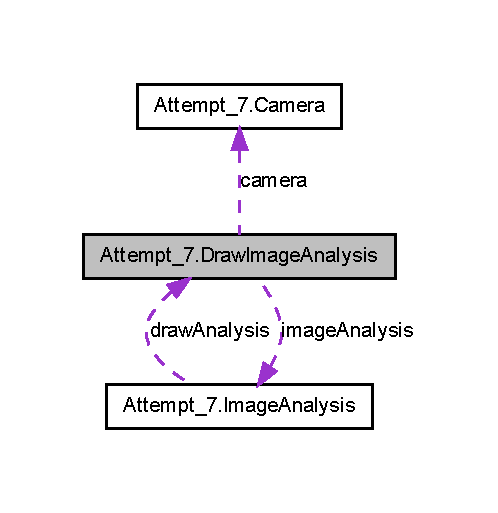
\includegraphics[width=239pt]{class_attempt__7_1_1_draw_image_analysis__coll__graph}
\end{center}
\end{figure}
\subsection*{Public Member Functions}
\begin{DoxyCompactItemize}
\item 
{\bf DrawImageAnalysis} (Game game, int {\bf screenWidth}, int {\bf screenHeight}, int {\bf updateSquareDimForDrawing}, int {\bf updateSquareDimForAnalysis}, int {\bf numberofLinesToFind}, int {\bf thetaIncrement}, int {\bf rhoIncrement}, List$<$ Viewport $>$ {\bf viewPortList}, {\bf ImageAnalysis} {\bf imageAnalysis})
\begin{DoxyCompactList}\small\item\em Initializes a new instance of the \doxyref{DrawImageAnalysis}{p.}{class_attempt__7_1_1_draw_image_analysis} class. \item\end{DoxyCompactList}\item 
override void {\bf Initialize} ()
\begin{DoxyCompactList}\small\item\em Allows the game component to perform any initialization it needs to before starting to run. This is where it can query for any required services and load content. \item\end{DoxyCompactList}\item 
override void {\bf Update} (GameTime gameTime)
\begin{DoxyCompactList}\small\item\em Allows the game component to update itself. \item\end{DoxyCompactList}\item 
void {\bf UpdateColorArrayto3DRectangle} (Color[,] c)
\item 
override void {\bf Draw} (GameTime gameTime)
\begin{DoxyCompactList}\small\item\em Calls methods to draw the analysis triangles and the Debug text. \item\end{DoxyCompactList}\item 
void {\bf UpdateBoolMapto3DRectangle} (bool[,] c, double[$\,$] {\bf houghInfo})
\begin{DoxyCompactList}\small\item\em Colors the analysis triangles based a trueFalse bool map. Also adds the Hough information If true then Blue. If false then Transparent. \item\end{DoxyCompactList}\end{DoxyCompactItemize}
\subsection*{Protected Member Functions}
\begin{DoxyCompactItemize}
\item 
override void {\bf LoadContent} ()
\begin{DoxyCompactList}\small\item\em Loads the SpriteBatch Content. \item\end{DoxyCompactList}\end{DoxyCompactItemize}
\subsection*{Private Member Functions}
\begin{DoxyCompactItemize}
\item 
void {\bf BuildVertexArrayforDrawingSmallerNumberofTriangles} (bool[,] c)
\begin{DoxyCompactList}\small\item\em Takes a bool map of and makes vertex positions based on the map. \item\end{DoxyCompactList}\item 
void {\bf InsertLine} (Vector3 startLocation, Vector3 endLocation, Color c)
\begin{DoxyCompactList}\small\item\em Updates the vertex information of the triangels for a line of a particular color based off its starting and ending position. \item\end{DoxyCompactList}\item 
void {\bf AddHoughLinesColor} ()
\begin{DoxyCompactList}\small\item\em Puts the hough information about the lines in the vertex array. \item\end{DoxyCompactList}\item 
void {\bf DrawVertexArray2} ()
\begin{DoxyCompactList}\small\item\em Draws the analysis rectangles that are in the \char`\"{}vertexArray2\char`\"{} and only draws the first count1D/3 in the array. \item\end{DoxyCompactList}\item 
void {\bf DrawText} (int turnIndication, int totalWhiteCnt, double[$\,$] {\bf houghInfo})
\item 
void {\bf LoadVertexArray} ()
\begin{DoxyCompactList}\small\item\em Loads the position of each triangle into the VertexArray. \item\end{DoxyCompactList}\end{DoxyCompactItemize}
\subsection*{Private Attributes}
\begin{DoxyCompactItemize}
\item 
int {\bf count1A}
\begin{DoxyCompactList}\small\item\em These values are part of the double for loops that reduce the computational requirements. These are the values that are incremented. \item\end{DoxyCompactList}\item 
int {\bf count2A}
\item 
int {\bf count1C}
\item 
int {\bf count2C}
\item 
int {\bf count1D} = 1
\begin{DoxyCompactList}\small\item\em Other count usage. 1D = the number of vertexs to draw. So the number of triangels will be 1/3 this number. \item\end{DoxyCompactList}\item 
int {\bf screenWidth}
\begin{DoxyCompactList}\small\item\em The screenSize. \item\end{DoxyCompactList}\item 
int {\bf screenHeight}
\item 
int {\bf updateSquareDimForDrawing}
\begin{DoxyCompactList}\small\item\em The dimensions of the double for loops. \item\end{DoxyCompactList}\item 
int {\bf updateSquareDimForAnalysis}
\item 
int {\bf numberofLinesToFind}
\begin{DoxyCompactList}\small\item\em How many lines to find. \item\end{DoxyCompactList}\item 
int {\bf thetaIncrement}
\begin{DoxyCompactList}\small\item\em How precise the hough transform is. How large between possible values. \item\end{DoxyCompactList}\item 
int {\bf rhoIncrement}
\item 
{\bf Camera} {\bf camera}
\begin{DoxyCompactList}\small\item\em \doxyref{Camera}{p.}{class_attempt__7_1_1_camera} used to draw the triangles of what the robot is \char`\"{}thinking\char`\"{}. \item\end{DoxyCompactList}\item 
List$<$ Viewport $>$ {\bf viewPortList}
\begin{DoxyCompactList}\small\item\em List holding the viewports used in the simulation. This list is created in the Main simulation and then passed to this class when it is initiaized. \item\end{DoxyCompactList}\item 
BasicEffect {\bf basicEffects}
\begin{DoxyCompactList}\small\item\em BasicEffects for how to draw the triangles. \item\end{DoxyCompactList}\item 
SpriteFont {\bf arial}
\begin{DoxyCompactList}\small\item\em Font to use for drawing the debug/hough information. \item\end{DoxyCompactList}\item 
SpriteBatch {\bf spriteBatch}
\begin{DoxyCompactList}\small\item\em The spriteBatch is used to draw 2D graphics. \item\end{DoxyCompactList}\item 
VertexPositionColor[$\,$] {\bf vertexArray}
\begin{DoxyCompactList}\small\item\em VertexPositionColory array that stores the triangles of what the robot is \char`\"{}thinking\char`\"{}. Each triangle represents 1 pixel from the robot's view. So 640$\ast$480 triangles. \item\end{DoxyCompactList}\item 
VertexPositionColor[$\,$] {\bf vertexArray2}
\begin{DoxyCompactList}\small\item\em Stores vertex information about the houglines and white pixels. Each time a vertex is added count1D should be incremented. \item\end{DoxyCompactList}\item 
double[$\,$] {\bf houghInfo}
\begin{DoxyCompactList}\small\item\em Stores information about the hough. \item\end{DoxyCompactList}\item 
{\bf ImageAnalysis} {\bf imageAnalysis}
\begin{DoxyCompactList}\small\item\em The image analysis object associated with this class. \item\end{DoxyCompactList}\item 
int[$\,$] {\bf vertexIndex}
\begin{DoxyCompactList}\small\item\em A list of the vertexs to draw. \item\end{DoxyCompactList}\item 
Vector3[$\,$] {\bf houghLineStartandStopVectors}
\begin{DoxyCompactList}\small\item\em Stores info about where houghlines start and stop. Values 0=start of houghline Vector3, 1= End of houghLine Vector3. \item\end{DoxyCompactList}\end{DoxyCompactItemize}


\subsection{Detailed Description}
This is a game component that implements IUpdateable. Draws the image analysis information. 

Definition at line 20 of file DrawImageAnalysis2.cs.



\subsection{Constructor \& Destructor Documentation}
\index{Attempt\_\-7::DrawImageAnalysis@{Attempt\_\-7::DrawImageAnalysis}!DrawImageAnalysis@{DrawImageAnalysis}}
\index{DrawImageAnalysis@{DrawImageAnalysis}!Attempt_7::DrawImageAnalysis@{Attempt\_\-7::DrawImageAnalysis}}
\subsubsection[{DrawImageAnalysis}]{\setlength{\rightskip}{0pt plus 5cm}Attempt\_\-7.DrawImageAnalysis.DrawImageAnalysis (
\begin{DoxyParamCaption}
\item[{Game}]{game, }
\item[{int}]{screenWidth, }
\item[{int}]{screenHeight, }
\item[{int}]{updateSquareDimForDrawing, }
\item[{int}]{updateSquareDimForAnalysis, }
\item[{int}]{numberofLinesToFind, }
\item[{int}]{thetaIncrement, }
\item[{int}]{rhoIncrement, }
\item[{List$<$ Viewport $>$}]{viewPortList, }
\item[{{\bf ImageAnalysis}}]{imageAnalysis}
\end{DoxyParamCaption}
)}\label{class_attempt__7_1_1_draw_image_analysis_ac9260a734adf91c819f2dc5230607af3}


Initializes a new instance of the \doxyref{DrawImageAnalysis}{p.}{class_attempt__7_1_1_draw_image_analysis} class. 


\begin{DoxyParams}{Parameters}
{\em game} & the game associated with the calss\\
\hline
{\em screenWidth} & ScreenWidth\\
\hline
{\em screenHeight} & ScreenHeight\\
\hline
{\em updateSquareDimForDrawing} & How fast to update drawing. Obsolete\\
\hline
{\em updateSquareDimForAnalysis} & How fast to update analysis. This is used mostly for hough\\
\hline
{\em numberofLinesToFind} & How many lines to find in the picture\\
\hline
{\em thetaIncrement} & Quantitization of angle size, in degrees\\
\hline
{\em rhoIncrement} & Quantitization of rho size\\
\hline
{\em viewPortList} & A list of view ports\\
\hline
{\em imageAnalysis} & Associated imageAnalysis object.\\
\hline
\end{DoxyParams}


Definition at line 120 of file DrawImageAnalysis2.cs.


\begin{DoxyCode}
            : base(game)
        {
            this.screenWidth = screenWidth;
            this.screenHeight = screenHeight;
            this.updateSquareDimForDrawing = updateSquareDimForDrawing;
            this.updateSquareDimForAnalysis = updateSquareDimForAnalysis;
            this.numberofLinesToFind = numberofLinesToFind;
            this.thetaIncrement = thetaIncrement;
            this.rhoIncrement = rhoIncrement;
            this.viewPortList = viewPortList;
            this.imageAnalysis = imageAnalysis;
        }
\end{DoxyCode}


\subsection{Member Function Documentation}
\index{Attempt\_\-7::DrawImageAnalysis@{Attempt\_\-7::DrawImageAnalysis}!AddHoughLinesColor@{AddHoughLinesColor}}
\index{AddHoughLinesColor@{AddHoughLinesColor}!Attempt_7::DrawImageAnalysis@{Attempt\_\-7::DrawImageAnalysis}}
\subsubsection[{AddHoughLinesColor}]{\setlength{\rightskip}{0pt plus 5cm}void Attempt\_\-7.DrawImageAnalysis.AddHoughLinesColor (
\begin{DoxyParamCaption}
{}
\end{DoxyParamCaption}
)\hspace{0.3cm}{\ttfamily  [private]}}\label{class_attempt__7_1_1_draw_image_analysis_a2e2d0a8b750ee6b4e4a91584dc5907d2}


Puts the hough information about the lines in the vertex array. 



Definition at line 335 of file DrawImageAnalysis2.cs.


\begin{DoxyCode}
        {
            // The first line found will be the darkest. The last line found will
       be the lightest
            int colorInc = (255 - 0) / this.numberofLinesToFind;

            for (int i = 0; i < this.numberofLinesToFind; i++)
            {
                // Insert a hough line to from the start and stop positions calcu
      lated before. 
                this.InsertLine(this.houghLineStartandStopVectors[i * 4], this.
      houghLineStartandStopVectors[1 + (i * 4)], new Color(255 - (i * colorInc), 0, 0))
      ;

                // Insert a line from 0,0 to closest point on hough line. This li
      ne will be perpendicular to hough line. 
                this.InsertLine(this.houghLineStartandStopVectors[(i * 4) + 2], V
      ector3.Zero, new Color(150, 255 - (i * colorInc), 150));

                // Insert a line from bottom middle to the closest point on hough
       line. This line will be perpendicular to hough line. 
                this.InsertLine(this.houghLineStartandStopVectors[(i * 4) + 3], n
      ew Vector3(this.screenWidth / 2, this.screenHeight, 0), new Color(0, 255, 255 - (
      i * colorInc)));
            }
        }       
\end{DoxyCode}


Here is the call graph for this function:
\nopagebreak
\begin{figure}[H]
\begin{center}
\leavevmode
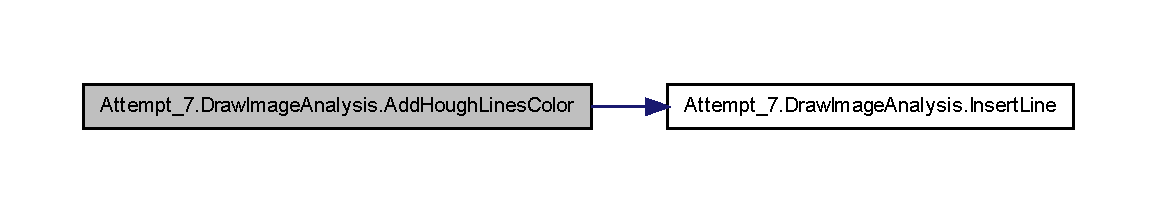
\includegraphics[width=400pt]{class_attempt__7_1_1_draw_image_analysis_a2e2d0a8b750ee6b4e4a91584dc5907d2_cgraph}
\end{center}
\end{figure}




Here is the caller graph for this function:
\nopagebreak
\begin{figure}[H]
\begin{center}
\leavevmode
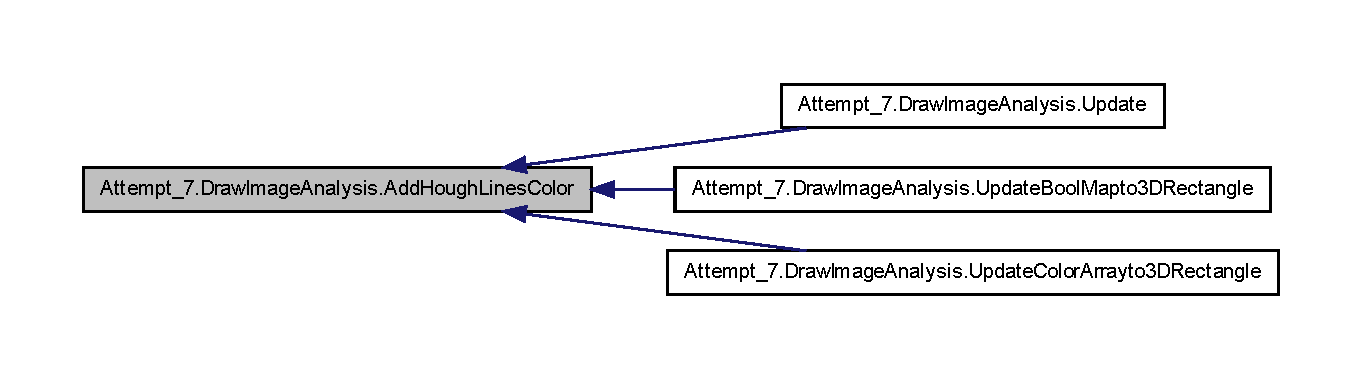
\includegraphics[width=400pt]{class_attempt__7_1_1_draw_image_analysis_a2e2d0a8b750ee6b4e4a91584dc5907d2_icgraph}
\end{center}
\end{figure}


\index{Attempt\_\-7::DrawImageAnalysis@{Attempt\_\-7::DrawImageAnalysis}!BuildVertexArrayforDrawingSmallerNumberofTriangles@{BuildVertexArrayforDrawingSmallerNumberofTriangles}}
\index{BuildVertexArrayforDrawingSmallerNumberofTriangles@{BuildVertexArrayforDrawingSmallerNumberofTriangles}!Attempt_7::DrawImageAnalysis@{Attempt\_\-7::DrawImageAnalysis}}
\subsubsection[{BuildVertexArrayforDrawingSmallerNumberofTriangles}]{\setlength{\rightskip}{0pt plus 5cm}void Attempt\_\-7.DrawImageAnalysis.BuildVertexArrayforDrawingSmallerNumberofTriangles (
\begin{DoxyParamCaption}
\item[{bool}]{c[,]}
\end{DoxyParamCaption}
)\hspace{0.3cm}{\ttfamily  [private]}}\label{class_attempt__7_1_1_draw_image_analysis_a5412536d4836b4592239d052bc278f6e}


Takes a bool map of and makes vertex positions based on the map. 


\begin{DoxyParams}{Parameters}
{\em c} & The bool map\\
\hline
\end{DoxyParams}


Definition at line 269 of file DrawImageAnalysis2.cs.


\begin{DoxyCode}
        {            
            this.count1D = 0;
            for (int x = 0; x < this.screenWidth; x++)
            {
                for (int y = 0; y < this.screenHeight;)
                {
                    if (c[x, y] == true)
                    {
                        int j = 1;

                        // If there are multiple pixels in a row, then make them 
      all into on larger triangle.
                        // Find how many pixels are in  a row.
                        while ((y + j) < this.screenHeight && c[x, y + j] == true
      )
                        {
                            j++;
                        }

                        this.vertexArray2[this.count1D + 0].Position = new Vector
      3(x, y, 0); // Put a vertex at the position.
                        this.vertexArray2[this.count1D + 0].Color = Color.Blue;
                        this.vertexArray2[this.count1D + 1].Position = new Vector
      3(x + 3, y + j, 0); // Put another vertex a the position but +1 in the X directio
      n
                        this.vertexArray2[this.count1D + 1].Color = Color.Blue;
                        this.vertexArray2[this.count1D + 2].Position = new Vector
      3(x, y + 3 + j, 0); // Put another vertex a the position but +1 in the X directio
      n
                        this.vertexArray2[this.count1D + 2].Color = Color.Blue;
                        this.count1D += 3;

                        y += j;
                    }
                    else
                    {
                        y++;
                    }
                }
            }
        }
\end{DoxyCode}


Here is the caller graph for this function:
\nopagebreak
\begin{figure}[H]
\begin{center}
\leavevmode
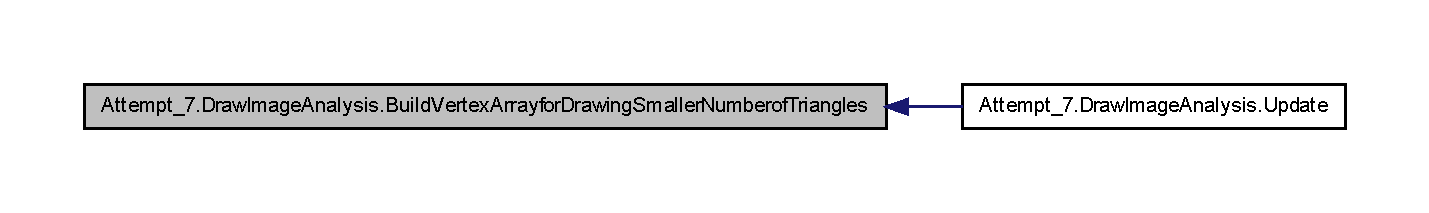
\includegraphics[width=400pt]{class_attempt__7_1_1_draw_image_analysis_a5412536d4836b4592239d052bc278f6e_icgraph}
\end{center}
\end{figure}


\index{Attempt\_\-7::DrawImageAnalysis@{Attempt\_\-7::DrawImageAnalysis}!Draw@{Draw}}
\index{Draw@{Draw}!Attempt_7::DrawImageAnalysis@{Attempt\_\-7::DrawImageAnalysis}}
\subsubsection[{Draw}]{\setlength{\rightskip}{0pt plus 5cm}override void Attempt\_\-7.DrawImageAnalysis.Draw (
\begin{DoxyParamCaption}
\item[{GameTime}]{gameTime}
\end{DoxyParamCaption}
)}\label{class_attempt__7_1_1_draw_image_analysis_a3405b325467c48533528a5312bbbf08b}


Calls methods to draw the analysis triangles and the Debug text. 


\begin{DoxyParams}{Parameters}
{\em gameTime} & Clock Information\\
\hline
\end{DoxyParams}


Definition at line 210 of file DrawImageAnalysis2.cs.


\begin{DoxyCode}
        {
            Game.GraphicsDevice.Viewport = this.viewPortList[1]; // Right center 
      view port           
            this.DrawVertexArray2(); // Draw the triangles showing the analysis

            Game.GraphicsDevice.Viewport = this.viewPortList[2]; // Right bottom
            this.DrawText(this.imageAnalysis.GetTurnIndicator(), this.
      imageAnalysis.GetWhiteCount(), this.houghInfo); // Draw the hough text info
            base.Draw(gameTime);
        }
\end{DoxyCode}


Here is the call graph for this function:
\nopagebreak
\begin{figure}[H]
\begin{center}
\leavevmode
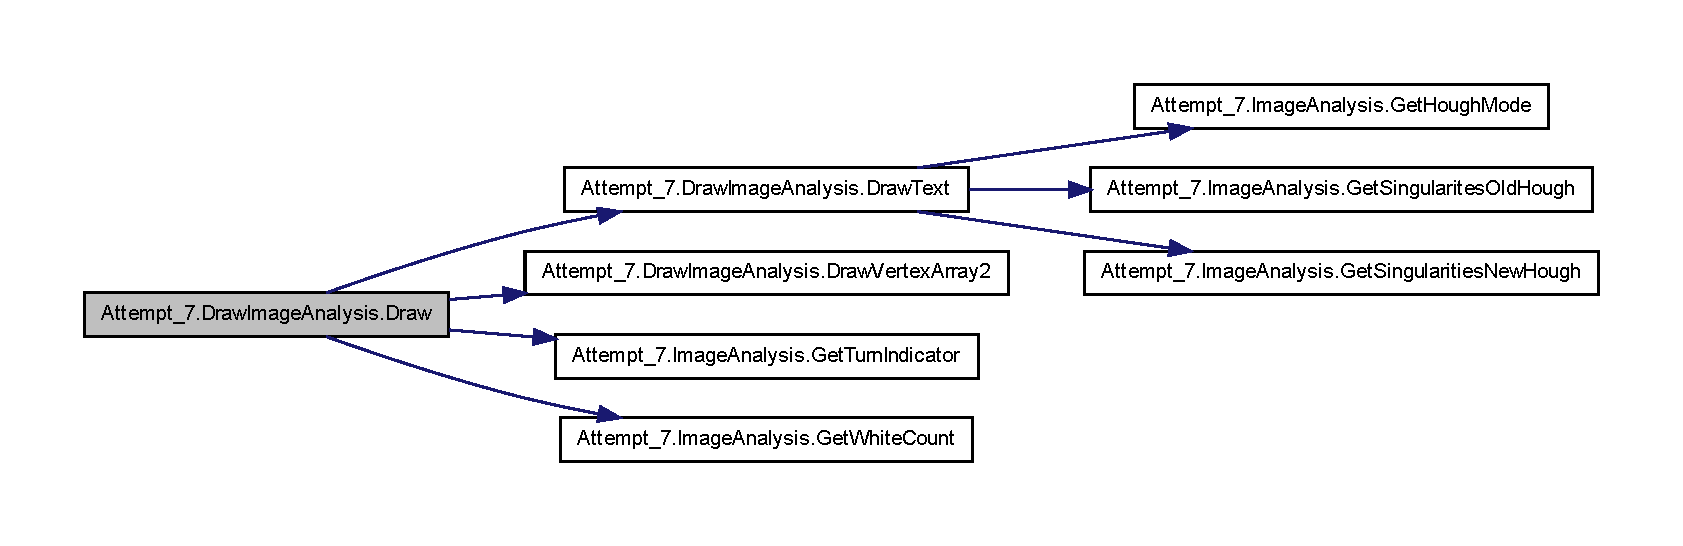
\includegraphics[width=400pt]{class_attempt__7_1_1_draw_image_analysis_a3405b325467c48533528a5312bbbf08b_cgraph}
\end{center}
\end{figure}


\index{Attempt\_\-7::DrawImageAnalysis@{Attempt\_\-7::DrawImageAnalysis}!DrawText@{DrawText}}
\index{DrawText@{DrawText}!Attempt_7::DrawImageAnalysis@{Attempt\_\-7::DrawImageAnalysis}}
\subsubsection[{DrawText}]{\setlength{\rightskip}{0pt plus 5cm}void Attempt\_\-7.DrawImageAnalysis.DrawText (
\begin{DoxyParamCaption}
\item[{int}]{turnIndication, }
\item[{int}]{totalWhiteCnt, }
\item[{double[$\,$]}]{houghInfo}
\end{DoxyParamCaption}
)\hspace{0.3cm}{\ttfamily  [private]}}\label{class_attempt__7_1_1_draw_image_analysis_aaf4088bca6ef2e41e13c6a9bf0ca2a52}
Draws the Text giving important information about the status of the analysis. 
\begin{DoxyParams}{Parameters}
{\em turnIndication} & Indicator of how much to turn\\
\hline
{\em totalWhiteCnt} & Number of white pixels found\\
\hline
{\em houghInfo} & Hough information array\\
\hline
\end{DoxyParams}


Definition at line 374 of file DrawImageAnalysis2.cs.


\begin{DoxyCode}
        {
            int spacing = 15;
            this.spriteBatch.Begin();
            this.spriteBatch.DrawString(this.arial, "slope", new Vector2(0, 0), C
      olor.White);
            this.spriteBatch.DrawString(this.arial, "yintercept", new Vector2(0, 
      spacing * 1), Color.White);
            this.spriteBatch.DrawString(this.arial, "rho", new Vector2(0, spacing
       * 2), Color.White);
            this.spriteBatch.DrawString(this.arial, "theta", new Vector2(0, spaci
      ng * 3), Color.White);
            this.spriteBatch.DrawString(this.arial, "x1", new Vector2(0, spacing 
      * 4), Color.White);
            this.spriteBatch.DrawString(this.arial, "y1", new Vector2(0, spacing 
      * 5), Color.White);
            this.spriteBatch.DrawString(this.arial, "BinSize", new Vector2(0, spa
      cing * 6), Color.White);
            this.spriteBatch.DrawString(this.arial, "xTrans = ", new Vector2(0, s
      pacing * 7), Color.White);
            this.spriteBatch.DrawString(this.arial, "yTrans = ", new Vector2(0, s
      pacing * 8), Color.White);
            this.spriteBatch.DrawString(this.arial, "Distance = ", new Vector2(0,
       spacing * 9), Color.White);
            this.spriteBatch.DrawString(this.arial, "Angle = ", new Vector2(0, sp
      acing * 10), Color.White);
            this.spriteBatch.DrawString(this.arial, "Turn Indicator = " + turnInd
      ication.ToString(), new Vector2(0, spacing * 11), Color.White);
            this.spriteBatch.DrawString(this.arial, "White Count = " + totalWhite
      Cnt.ToString() + " Vertexs = " + this.count1D.ToString(), new Vector2(0, spacing 
      * 12), Color.White);
            this.spriteBatch.DrawString(this.arial, "Number Of lines To find = " 
      + this.numberofLinesToFind.ToString() + " -  theta Average = " + this.houghInfo[(
      this.numberofLinesToFind * 11)].ToString() + "  - rho Average = " + this.
      houghInfo[(this.numberofLinesToFind * 11) + 1].ToString(), new Vector2(0, spacing
       * 13), Color.White);
            this.spriteBatch.DrawString(this.arial, "Singualarites Old:" + this.
      imageAnalysis.GetSingularitesOldHough() + " New = " + this.imageAnalysis.GetSingu
      laritiesNewHough(), new Vector2(0, spacing * 14), Color.White);
            this.spriteBatch.DrawString(this.arial, "Hough Mode " + this.
      imageAnalysis.GetHoughMode(), new Vector2(0, spacing * 15), Color.White);

            int spacingForText = (GraphicsDevice.Viewport.Width - 50) / this.
      numberofLinesToFind;

            // Insert the hough data for each line. 
            for (int j = 0; j < this.numberofLinesToFind; j++)
            {
                for (int i = 0; i < 11; i++)
                {
                    this.spriteBatch.DrawString(this.arial, houghInfo[(j * 11) + 
      i].ToString(), new Vector2(50 + (spacingForText * j), i * spacing), Color.White);
      
                }
            }

            this.spriteBatch.End();
        }
\end{DoxyCode}


Here is the call graph for this function:
\nopagebreak
\begin{figure}[H]
\begin{center}
\leavevmode
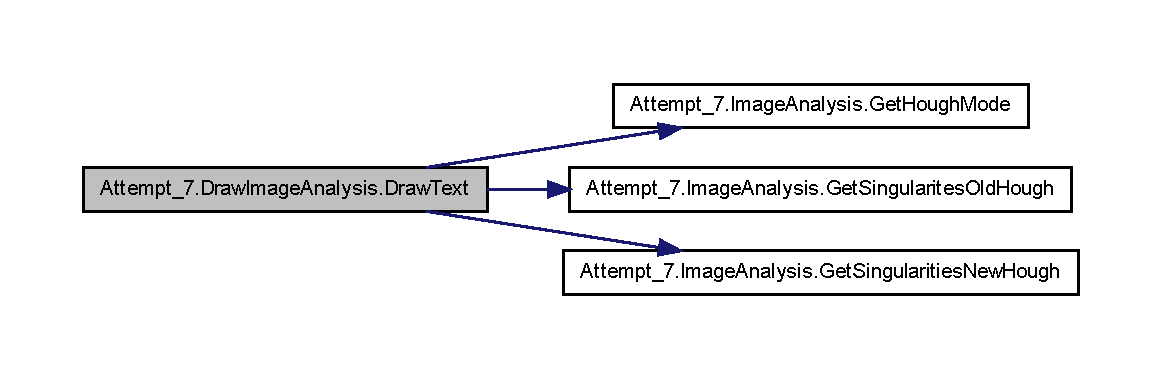
\includegraphics[width=400pt]{class_attempt__7_1_1_draw_image_analysis_aaf4088bca6ef2e41e13c6a9bf0ca2a52_cgraph}
\end{center}
\end{figure}




Here is the caller graph for this function:\nopagebreak
\begin{figure}[H]
\begin{center}
\leavevmode
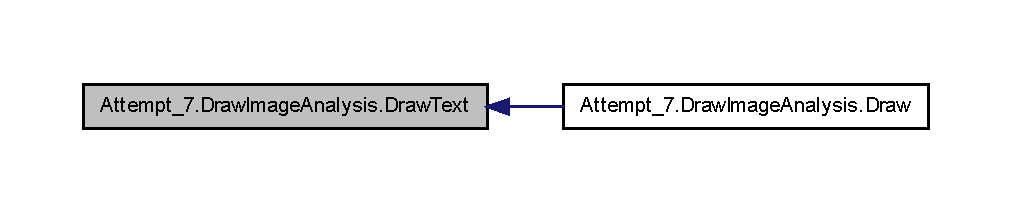
\includegraphics[width=400pt]{class_attempt__7_1_1_draw_image_analysis_aaf4088bca6ef2e41e13c6a9bf0ca2a52_icgraph}
\end{center}
\end{figure}


\index{Attempt\_\-7::DrawImageAnalysis@{Attempt\_\-7::DrawImageAnalysis}!DrawVertexArray2@{DrawVertexArray2}}
\index{DrawVertexArray2@{DrawVertexArray2}!Attempt_7::DrawImageAnalysis@{Attempt\_\-7::DrawImageAnalysis}}
\subsubsection[{DrawVertexArray2}]{\setlength{\rightskip}{0pt plus 5cm}void Attempt\_\-7.DrawImageAnalysis.DrawVertexArray2 (
\begin{DoxyParamCaption}
{}
\end{DoxyParamCaption}
)\hspace{0.3cm}{\ttfamily  [private]}}\label{class_attempt__7_1_1_draw_image_analysis_a4729388d94926e86a7ecd6933233638b}


Draws the analysis rectangles that are in the \char`\"{}vertexArray2\char`\"{} and only draws the first count1D/3 in the array. 



Definition at line 356 of file DrawImageAnalysis2.cs.


\begin{DoxyCode}
        {
            if (this.count1D != 0)
            {
                foreach (EffectPass pass in this.basicEffects.CurrentTechnique.Pa
      sses)
                {
                    pass.Apply();
                    GraphicsDevice.DrawUserPrimitives<VertexPositionColor>(Primit
      iveType.TriangleList, this.vertexArray2, 0, this.count1D / 3);
                }
            }
        }
\end{DoxyCode}


Here is the caller graph for this function:
\nopagebreak
\begin{figure}[H]
\begin{center}
\leavevmode
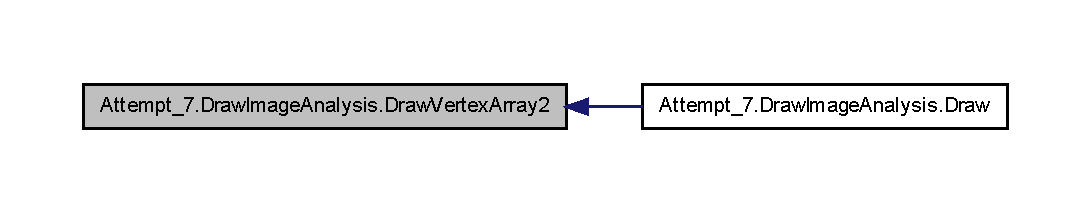
\includegraphics[width=400pt]{class_attempt__7_1_1_draw_image_analysis_a4729388d94926e86a7ecd6933233638b_icgraph}
\end{center}
\end{figure}


\index{Attempt\_\-7::DrawImageAnalysis@{Attempt\_\-7::DrawImageAnalysis}!Initialize@{Initialize}}
\index{Initialize@{Initialize}!Attempt_7::DrawImageAnalysis@{Attempt\_\-7::DrawImageAnalysis}}
\subsubsection[{Initialize}]{\setlength{\rightskip}{0pt plus 5cm}override void Attempt\_\-7.DrawImageAnalysis.Initialize (
\begin{DoxyParamCaption}
{}
\end{DoxyParamCaption}
)}\label{class_attempt__7_1_1_draw_image_analysis_ae271911b749fc6bad5f303da0f6b895d}


Allows the game component to perform any initialization it needs to before starting to run. This is where it can query for any required services and load content. 



Definition at line 138 of file DrawImageAnalysis2.cs.


\begin{DoxyCode}
        {
            // Create a new SpriteBatch, which can be used to draw 2D textures.
            this.spriteBatch = new SpriteBatch(Game.GraphicsDevice);

            this.houghInfo = this.imageAnalysis.GetHoughInfo();           
            this.arial = Game.Content.Load<SpriteFont>("Arial"); // Load the font
      

            // Camera needed for the analysis picture 
            int xposition = this.screenHeight * 50 / 100;
            int yposition = this.screenWidth * 50 / 100;
            this.camera = new Camera(Game, new Vector3(yposition, xposition, -590
      ), new Vector3(yposition, xposition, 0), -Vector3.UnitY, true); // Unit x for upd
      irection
            this.Game.Components.Add(this.camera);

            this.vertexIndex = new int[this.screenHeight * this.screenWidth * 2];
                  

            this.LoadVertexArray(); // Loads the vertexs needed to draw the analy
      sis triangles
            this.vertexArray2 = new VertexPositionColor[65535]; // The vertex arr
      ay for the analysis triangles , the largest this could be is 65535 = 16 bit
            for (int i = 0; i < 65535; i++)
            {
                this.vertexArray2[i] = new VertexPositionColor(Vector3.UnitX, Col
      or.Blue);
            }

            base.Initialize();
        }
\end{DoxyCode}


Here is the call graph for this function:
\nopagebreak
\begin{figure}[H]
\begin{center}
\leavevmode
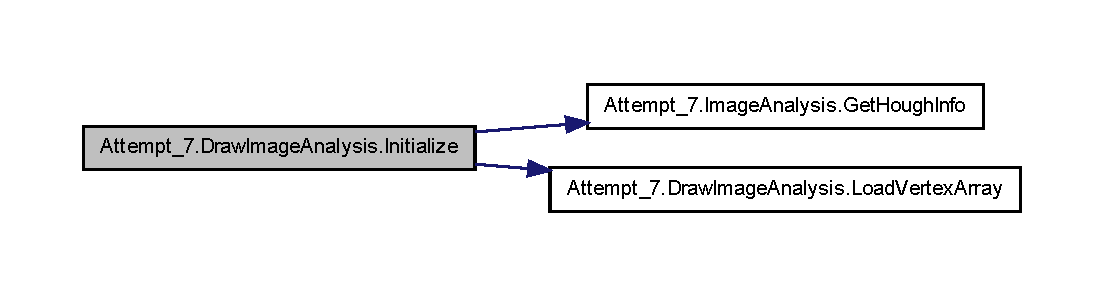
\includegraphics[width=400pt]{class_attempt__7_1_1_draw_image_analysis_ae271911b749fc6bad5f303da0f6b895d_cgraph}
\end{center}
\end{figure}


\index{Attempt\_\-7::DrawImageAnalysis@{Attempt\_\-7::DrawImageAnalysis}!InsertLine@{InsertLine}}
\index{InsertLine@{InsertLine}!Attempt_7::DrawImageAnalysis@{Attempt\_\-7::DrawImageAnalysis}}
\subsubsection[{InsertLine}]{\setlength{\rightskip}{0pt plus 5cm}void Attempt\_\-7.DrawImageAnalysis.InsertLine (
\begin{DoxyParamCaption}
\item[{Vector3}]{startLocation, }
\item[{Vector3}]{endLocation, }
\item[{Color}]{c}
\end{DoxyParamCaption}
)\hspace{0.3cm}{\ttfamily  [private]}}\label{class_attempt__7_1_1_draw_image_analysis_aa1273c30c63d4963aebfede894eec3e4}


Updates the vertex information of the triangels for a line of a particular color based off its starting and ending position. 


\begin{DoxyParams}{Parameters}
{\em startLocation} & Start position of the line. \\
\hline
{\em endLocation} & End position of the line \\
\hline
{\em c} & Color to draw the line. \\
\hline
\end{DoxyParams}


Definition at line 311 of file DrawImageAnalysis2.cs.


\begin{DoxyCode}
        {           
            // Make a line, but make the number of points dependent on the length
       of the line. 
            int incrementNumber = (int)Vector3.Distance(startLocation, endLocatio
      n) / 10;
            for (int i = 0; i < incrementNumber; i++)
            {
                // Find each points location 
                Vector3 lineLocation1 = Vector3.Lerp(startLocation, endLocation, 
      (float)(i * 1f / incrementNumber));
                {
                    // Make the point 5 wide
                    this.vertexArray2[this.count1D + 0].Position = new Vector3(li
      neLocation1.X, lineLocation1.Y, 0); // Put a vertex at the position.
                    this.vertexArray2[this.count1D + 0].Color = c;
                    this.vertexArray2[this.count1D + 1].Position = new Vector3(li
      neLocation1.X + 10, lineLocation1.Y, 0); // Put another vertex a the position but
       +1 in the X direction
                    this.vertexArray2[this.count1D + 1].Color = c;
                    this.vertexArray2[this.count1D + 2].Position = new Vector3(li
      neLocation1.X, lineLocation1.Y + 10, 0); // Put another vertex a the position but
       +1 in the X direction
                    this.vertexArray2[this.count1D + 2].Color = c;
                    this.count1D += 3;                    
                }
            }
        }
\end{DoxyCode}


Here is the caller graph for this function:
\nopagebreak
\begin{figure}[H]
\begin{center}
\leavevmode
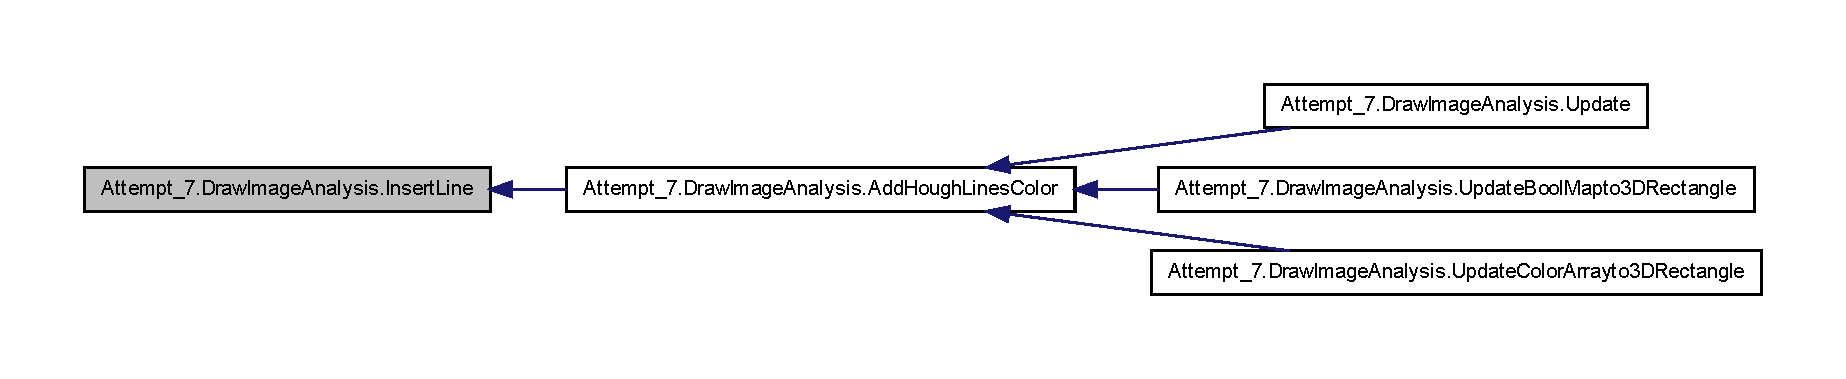
\includegraphics[width=400pt]{class_attempt__7_1_1_draw_image_analysis_aa1273c30c63d4963aebfede894eec3e4_icgraph}
\end{center}
\end{figure}


\index{Attempt\_\-7::DrawImageAnalysis@{Attempt\_\-7::DrawImageAnalysis}!LoadContent@{LoadContent}}
\index{LoadContent@{LoadContent}!Attempt_7::DrawImageAnalysis@{Attempt\_\-7::DrawImageAnalysis}}
\subsubsection[{LoadContent}]{\setlength{\rightskip}{0pt plus 5cm}override void Attempt\_\-7.DrawImageAnalysis.LoadContent (
\begin{DoxyParamCaption}
{}
\end{DoxyParamCaption}
)\hspace{0.3cm}{\ttfamily  [protected]}}\label{class_attempt__7_1_1_draw_image_analysis_affaba058b8e77f01efcba3f6ded28dea}


Loads the SpriteBatch Content. 



Definition at line 260 of file DrawImageAnalysis2.cs.


\begin{DoxyCode}
        {
            base.LoadContent();
        }
\end{DoxyCode}
\index{Attempt\_\-7::DrawImageAnalysis@{Attempt\_\-7::DrawImageAnalysis}!LoadVertexArray@{LoadVertexArray}}
\index{LoadVertexArray@{LoadVertexArray}!Attempt_7::DrawImageAnalysis@{Attempt\_\-7::DrawImageAnalysis}}
\subsubsection[{LoadVertexArray}]{\setlength{\rightskip}{0pt plus 5cm}void Attempt\_\-7.DrawImageAnalysis.LoadVertexArray (
\begin{DoxyParamCaption}
{}
\end{DoxyParamCaption}
)\hspace{0.3cm}{\ttfamily  [private]}}\label{class_attempt__7_1_1_draw_image_analysis_aea47cb9ef13fda648ba3e8acb8808ed3}


Loads the position of each triangle into the VertexArray. 



Definition at line 413 of file DrawImageAnalysis2.cs.


\begin{DoxyCode}
        {
            this.vertexArray = new VertexPositionColor[(this.screenWidth * this.
      screenHeight) + 5]; // The vertex array for the analysis triangles

            for (int x = this.screenHeight - 1; x > 0; x--)
            {
                for (int y = this.screenWidth - 1; y > 0; y -= 2)
                {
                    this.vertexArray[(x * this.screenWidth) - y] = new VertexPosi
      tionColor(new Vector3(x, y, 0), Color.White); // Put a vertex at the position.
                    this.vertexArray[(x * this.screenWidth) - (y + 1)] = new Vert
      exPositionColor(new Vector3(x + 1, y, 0), Color.White); // Put another vertex a t
      he position but +1 in the X direction
                }
            }

            // Create the basic effect. 
            this.basicEffects = new BasicEffect(Game.GraphicsDevice);
            this.basicEffects.TextureEnabled = false;
            this.basicEffects.VertexColorEnabled = true;
            this.basicEffects.World = this.camera.World;
            this.basicEffects.View = this.camera.View;
            this.basicEffects.Projection = this.camera.Projection;
        }
\end{DoxyCode}


Here is the caller graph for this function:\nopagebreak
\begin{figure}[H]
\begin{center}
\leavevmode
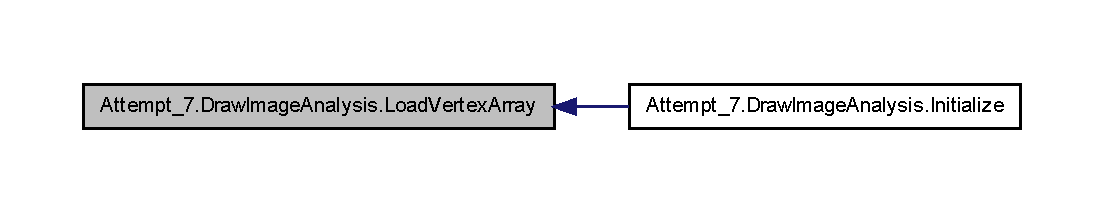
\includegraphics[width=400pt]{class_attempt__7_1_1_draw_image_analysis_aea47cb9ef13fda648ba3e8acb8808ed3_icgraph}
\end{center}
\end{figure}


\index{Attempt\_\-7::DrawImageAnalysis@{Attempt\_\-7::DrawImageAnalysis}!Update@{Update}}
\index{Update@{Update}!Attempt_7::DrawImageAnalysis@{Attempt\_\-7::DrawImageAnalysis}}
\subsubsection[{Update}]{\setlength{\rightskip}{0pt plus 5cm}override void Attempt\_\-7.DrawImageAnalysis.Update (
\begin{DoxyParamCaption}
\item[{GameTime}]{gameTime}
\end{DoxyParamCaption}
)}\label{class_attempt__7_1_1_draw_image_analysis_a6de17ba6756456372d8d6e2a69d6ce45}


Allows the game component to update itself. 


\begin{DoxyParams}{Parameters}
{\em gameTime} & Provides a snapshot of timing values.\\
\hline
\end{DoxyParams}


Definition at line 168 of file DrawImageAnalysis2.cs.


\begin{DoxyCode}
        {
            this.houghInfo = this.imageAnalysis.GetHoughInfo();
            this.houghLineStartandStopVectors = this.imageAnalysis.GetHoughStarta
      ndStopVectors();
            this.BuildVertexArrayforDrawingSmallerNumberofTriangles(this.
      imageAnalysis.GetTrueFalseMaptoDraw());
            this.AddHoughLinesColor(); // Add the hough lines. 

            base.Update(gameTime);
        }
\end{DoxyCode}


Here is the call graph for this function:
\nopagebreak
\begin{figure}[H]
\begin{center}
\leavevmode
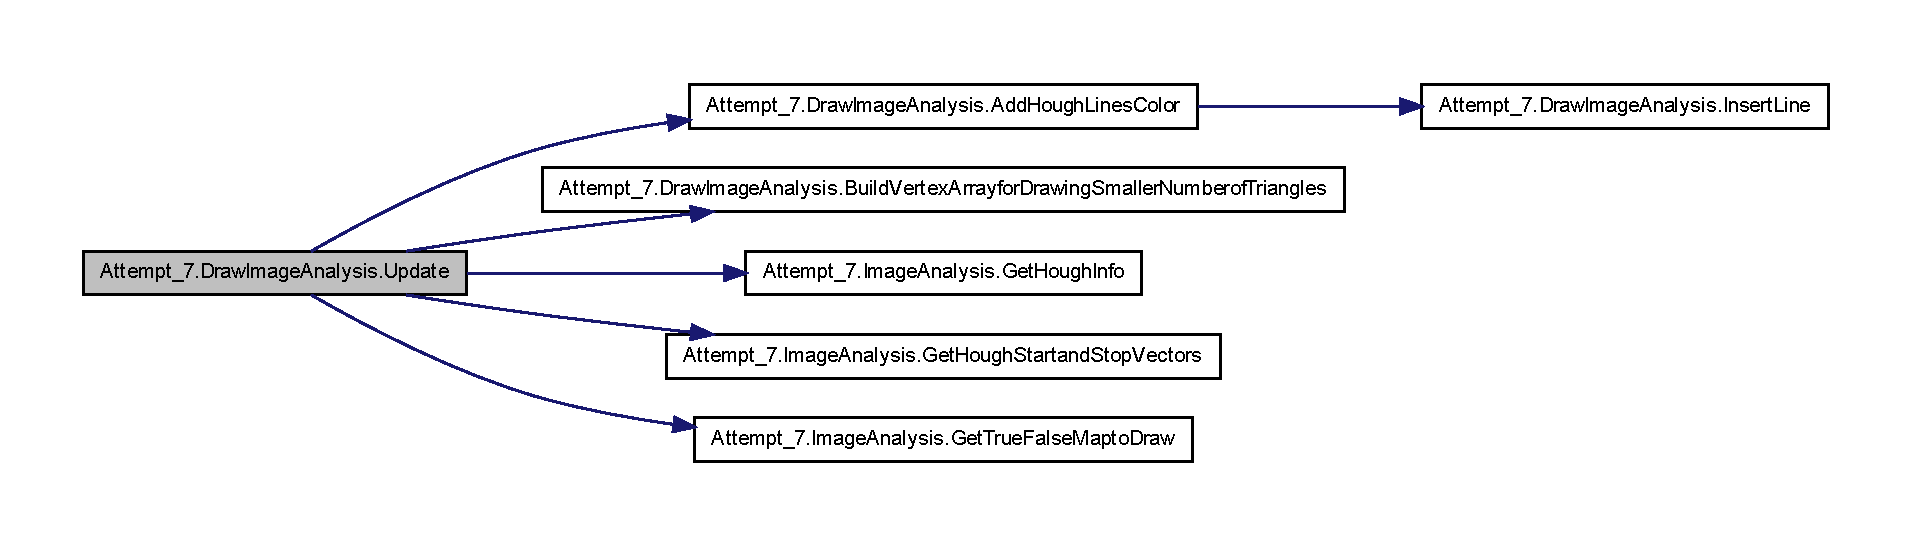
\includegraphics[width=400pt]{class_attempt__7_1_1_draw_image_analysis_a6de17ba6756456372d8d6e2a69d6ce45_cgraph}
\end{center}
\end{figure}


\index{Attempt\_\-7::DrawImageAnalysis@{Attempt\_\-7::DrawImageAnalysis}!UpdateBoolMapto3DRectangle@{UpdateBoolMapto3DRectangle}}
\index{UpdateBoolMapto3DRectangle@{UpdateBoolMapto3DRectangle}!Attempt_7::DrawImageAnalysis@{Attempt\_\-7::DrawImageAnalysis}}
\subsubsection[{UpdateBoolMapto3DRectangle}]{\setlength{\rightskip}{0pt plus 5cm}void Attempt\_\-7.DrawImageAnalysis.UpdateBoolMapto3DRectangle (
\begin{DoxyParamCaption}
\item[{bool}]{c[,], }
\item[{double[$\,$]}]{houghInfo}
\end{DoxyParamCaption}
)}\label{class_attempt__7_1_1_draw_image_analysis_ad0933abc7604eb194143440f1b875383}


Colors the analysis triangles based a trueFalse bool map. Also adds the Hough information If true then Blue. If false then Transparent. 


\begin{DoxyParams}{Parameters}
{\em c} & True False map\\
\hline
{\em houghInfo} & Hough Information\\
\hline
\end{DoxyParams}


Definition at line 226 of file DrawImageAnalysis2.cs.


\begin{DoxyCode}
        {
            for (int x = this.count1A; x < this.screenWidth; x += this.
      updateSquareDimForDrawing)
            {
                for (int y = this.count2A; y < this.screenHeight; y += this.
      updateSquareDimForDrawing)
                {
                    if (c[x, y] == true)
                    {
                        this.vertexArray[x + (y * this.screenWidth)].Color = Colo
      r.White;
                    }
                    else
                    {
                        this.vertexArray[x + (y * this.screenWidth)].Color = Colo
      r.Transparent;
                    }
                }
            }

            this.AddHoughLinesColor(); // Add the hough lines. 
            this.count1A++;
            if (this.count1A == this.updateSquareDimForDrawing)
            {
                this.count1A = 0;
                this.count2A++;

                if (this.count2A == this.updateSquareDimForDrawing)
                {
                    this.count2A = 0;
                }
            }
        }
\end{DoxyCode}


Here is the call graph for this function:
\nopagebreak
\begin{figure}[H]
\begin{center}
\leavevmode
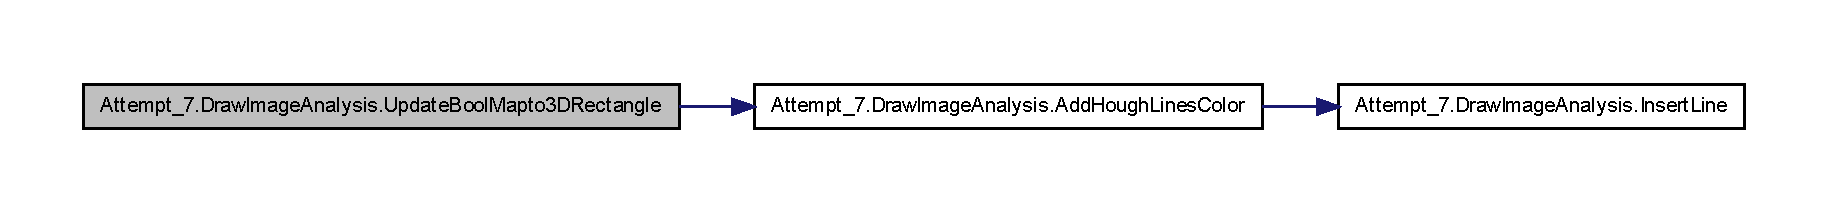
\includegraphics[width=400pt]{class_attempt__7_1_1_draw_image_analysis_ad0933abc7604eb194143440f1b875383_cgraph}
\end{center}
\end{figure}


\index{Attempt\_\-7::DrawImageAnalysis@{Attempt\_\-7::DrawImageAnalysis}!UpdateColorArrayto3DRectangle@{UpdateColorArrayto3DRectangle}}
\index{UpdateColorArrayto3DRectangle@{UpdateColorArrayto3DRectangle}!Attempt_7::DrawImageAnalysis@{Attempt\_\-7::DrawImageAnalysis}}
\subsubsection[{UpdateColorArrayto3DRectangle}]{\setlength{\rightskip}{0pt plus 5cm}void Attempt\_\-7.DrawImageAnalysis.UpdateColorArrayto3DRectangle (
\begin{DoxyParamCaption}
\item[{Color}]{c[,]}
\end{DoxyParamCaption}
)}\label{class_attempt__7_1_1_draw_image_analysis_a5fc3cbd0f863118307ed7b61e778e52e}
Takes a 2D color array and colors the triangles. 
\begin{DoxyParams}{Parameters}
{\em c} & Color array to make into triangles\\
\hline
\end{DoxyParams}


Definition at line 182 of file DrawImageAnalysis2.cs.


\begin{DoxyCode}
        {
            for (int x = this.count1C; x < this.screenWidth; x += this.
      updateSquareDimForDrawing)
            {
                for (int y = this.count2C; y < this.screenHeight; y += this.
      updateSquareDimForDrawing)
                {
                    this.vertexArray[x + (y * this.screenWidth)].Color = c[x, y];
      
                }
            }

            this.count1C++;
            if (this.count1C == this.updateSquareDimForDrawing)
            {
                this.count1C = 0;
                this.count2C++;
                this.AddHoughLinesColor(); // Add the hough lines. 

                if (this.count2C == this.updateSquareDimForDrawing)
                {
                    this.count2C = 0;
                }
            }
        }
\end{DoxyCode}


Here is the call graph for this function:
\nopagebreak
\begin{figure}[H]
\begin{center}
\leavevmode
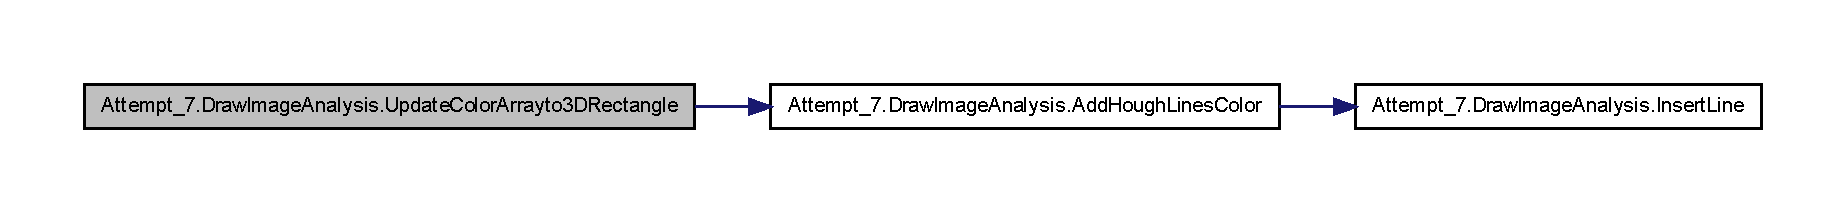
\includegraphics[width=400pt]{class_attempt__7_1_1_draw_image_analysis_a5fc3cbd0f863118307ed7b61e778e52e_cgraph}
\end{center}
\end{figure}




\subsection{Member Data Documentation}
\index{Attempt\_\-7::DrawImageAnalysis@{Attempt\_\-7::DrawImageAnalysis}!arial@{arial}}
\index{arial@{arial}!Attempt_7::DrawImageAnalysis@{Attempt\_\-7::DrawImageAnalysis}}
\subsubsection[{arial}]{\setlength{\rightskip}{0pt plus 5cm}SpriteFont {\bf Attempt\_\-7.DrawImageAnalysis.arial}\hspace{0.3cm}{\ttfamily  [private]}}\label{class_attempt__7_1_1_draw_image_analysis_a531efa4688cdabd3c3bf99a5f1777d9c}


Font to use for drawing the debug/hough information. 



Definition at line 70 of file DrawImageAnalysis2.cs.

\index{Attempt\_\-7::DrawImageAnalysis@{Attempt\_\-7::DrawImageAnalysis}!basicEffects@{basicEffects}}
\index{basicEffects@{basicEffects}!Attempt_7::DrawImageAnalysis@{Attempt\_\-7::DrawImageAnalysis}}
\subsubsection[{basicEffects}]{\setlength{\rightskip}{0pt plus 5cm}BasicEffect {\bf Attempt\_\-7.DrawImageAnalysis.basicEffects}\hspace{0.3cm}{\ttfamily  [private]}}\label{class_attempt__7_1_1_draw_image_analysis_a36779d384eaa0c4188a16758540403e0}


BasicEffects for how to draw the triangles. 



Definition at line 65 of file DrawImageAnalysis2.cs.

\index{Attempt\_\-7::DrawImageAnalysis@{Attempt\_\-7::DrawImageAnalysis}!camera@{camera}}
\index{camera@{camera}!Attempt_7::DrawImageAnalysis@{Attempt\_\-7::DrawImageAnalysis}}
\subsubsection[{camera}]{\setlength{\rightskip}{0pt plus 5cm}{\bf Camera} {\bf Attempt\_\-7.DrawImageAnalysis.camera}\hspace{0.3cm}{\ttfamily  [private]}}\label{class_attempt__7_1_1_draw_image_analysis_a96d5f79f1b1a104d2ab3f47aa6616d37}


\doxyref{Camera}{p.}{class_attempt__7_1_1_camera} used to draw the triangles of what the robot is \char`\"{}thinking\char`\"{}. 



Definition at line 55 of file DrawImageAnalysis2.cs.

\index{Attempt\_\-7::DrawImageAnalysis@{Attempt\_\-7::DrawImageAnalysis}!count1A@{count1A}}
\index{count1A@{count1A}!Attempt_7::DrawImageAnalysis@{Attempt\_\-7::DrawImageAnalysis}}
\subsubsection[{count1A}]{\setlength{\rightskip}{0pt plus 5cm}int {\bf Attempt\_\-7.DrawImageAnalysis.count1A}\hspace{0.3cm}{\ttfamily  [private]}}\label{class_attempt__7_1_1_draw_image_analysis_a0c212b6483e545cdb54b744f26ae5aaf}


These values are part of the double for loops that reduce the computational requirements. These are the values that are incremented. 



Definition at line 25 of file DrawImageAnalysis2.cs.

\index{Attempt\_\-7::DrawImageAnalysis@{Attempt\_\-7::DrawImageAnalysis}!count1C@{count1C}}
\index{count1C@{count1C}!Attempt_7::DrawImageAnalysis@{Attempt\_\-7::DrawImageAnalysis}}
\subsubsection[{count1C}]{\setlength{\rightskip}{0pt plus 5cm}int {\bf Attempt\_\-7.DrawImageAnalysis.count1C}\hspace{0.3cm}{\ttfamily  [private]}}\label{class_attempt__7_1_1_draw_image_analysis_afda6ca182d55b530c3188413bfced70c}


Definition at line 25 of file DrawImageAnalysis2.cs.

\index{Attempt\_\-7::DrawImageAnalysis@{Attempt\_\-7::DrawImageAnalysis}!count1D@{count1D}}
\index{count1D@{count1D}!Attempt_7::DrawImageAnalysis@{Attempt\_\-7::DrawImageAnalysis}}
\subsubsection[{count1D}]{\setlength{\rightskip}{0pt plus 5cm}int {\bf Attempt\_\-7.DrawImageAnalysis.count1D} = 1\hspace{0.3cm}{\ttfamily  [private]}}\label{class_attempt__7_1_1_draw_image_analysis_a0978bfdff294a91bc2c99d55c29a9e2f}


Other count usage. 1D = the number of vertexs to draw. So the number of triangels will be 1/3 this number. 



Definition at line 30 of file DrawImageAnalysis2.cs.

\index{Attempt\_\-7::DrawImageAnalysis@{Attempt\_\-7::DrawImageAnalysis}!count2A@{count2A}}
\index{count2A@{count2A}!Attempt_7::DrawImageAnalysis@{Attempt\_\-7::DrawImageAnalysis}}
\subsubsection[{count2A}]{\setlength{\rightskip}{0pt plus 5cm}int {\bf Attempt\_\-7.DrawImageAnalysis.count2A}\hspace{0.3cm}{\ttfamily  [private]}}\label{class_attempt__7_1_1_draw_image_analysis_ab82cc146a1cdfc52336d1ae86eb89157}


Definition at line 25 of file DrawImageAnalysis2.cs.

\index{Attempt\_\-7::DrawImageAnalysis@{Attempt\_\-7::DrawImageAnalysis}!count2C@{count2C}}
\index{count2C@{count2C}!Attempt_7::DrawImageAnalysis@{Attempt\_\-7::DrawImageAnalysis}}
\subsubsection[{count2C}]{\setlength{\rightskip}{0pt plus 5cm}int {\bf Attempt\_\-7.DrawImageAnalysis.count2C}\hspace{0.3cm}{\ttfamily  [private]}}\label{class_attempt__7_1_1_draw_image_analysis_aed235d7846bb2f2ace68331beb4ca7f2}


Definition at line 25 of file DrawImageAnalysis2.cs.

\index{Attempt\_\-7::DrawImageAnalysis@{Attempt\_\-7::DrawImageAnalysis}!houghInfo@{houghInfo}}
\index{houghInfo@{houghInfo}!Attempt_7::DrawImageAnalysis@{Attempt\_\-7::DrawImageAnalysis}}
\subsubsection[{houghInfo}]{\setlength{\rightskip}{0pt plus 5cm}double [$\,$] {\bf Attempt\_\-7.DrawImageAnalysis.houghInfo}\hspace{0.3cm}{\ttfamily  [private]}}\label{class_attempt__7_1_1_draw_image_analysis_a29f389c1637b758aea8700cc3b4d8c92}


Stores information about the hough. 



Definition at line 90 of file DrawImageAnalysis2.cs.

\index{Attempt\_\-7::DrawImageAnalysis@{Attempt\_\-7::DrawImageAnalysis}!houghLineStartandStopVectors@{houghLineStartandStopVectors}}
\index{houghLineStartandStopVectors@{houghLineStartandStopVectors}!Attempt_7::DrawImageAnalysis@{Attempt\_\-7::DrawImageAnalysis}}
\subsubsection[{houghLineStartandStopVectors}]{\setlength{\rightskip}{0pt plus 5cm}Vector3 [$\,$] {\bf Attempt\_\-7.DrawImageAnalysis.houghLineStartandStopVectors}\hspace{0.3cm}{\ttfamily  [private]}}\label{class_attempt__7_1_1_draw_image_analysis_a295eefafafe824bfc196c0d7e88f55aa}


Stores info about where houghlines start and stop. Values 0=start of houghline Vector3, 1= End of houghLine Vector3. 



Definition at line 105 of file DrawImageAnalysis2.cs.

\index{Attempt\_\-7::DrawImageAnalysis@{Attempt\_\-7::DrawImageAnalysis}!imageAnalysis@{imageAnalysis}}
\index{imageAnalysis@{imageAnalysis}!Attempt_7::DrawImageAnalysis@{Attempt\_\-7::DrawImageAnalysis}}
\subsubsection[{imageAnalysis}]{\setlength{\rightskip}{0pt plus 5cm}{\bf ImageAnalysis} {\bf Attempt\_\-7.DrawImageAnalysis.imageAnalysis}\hspace{0.3cm}{\ttfamily  [private]}}\label{class_attempt__7_1_1_draw_image_analysis_a111f5f187dc4143d67b30d98031d0968}


The image analysis object associated with this class. 



Definition at line 95 of file DrawImageAnalysis2.cs.

\index{Attempt\_\-7::DrawImageAnalysis@{Attempt\_\-7::DrawImageAnalysis}!numberofLinesToFind@{numberofLinesToFind}}
\index{numberofLinesToFind@{numberofLinesToFind}!Attempt_7::DrawImageAnalysis@{Attempt\_\-7::DrawImageAnalysis}}
\subsubsection[{numberofLinesToFind}]{\setlength{\rightskip}{0pt plus 5cm}int {\bf Attempt\_\-7.DrawImageAnalysis.numberofLinesToFind}\hspace{0.3cm}{\ttfamily  [private]}}\label{class_attempt__7_1_1_draw_image_analysis_ac6adfc217d9308380d780ef2c5798a07}


How many lines to find. 



Definition at line 45 of file DrawImageAnalysis2.cs.

\index{Attempt\_\-7::DrawImageAnalysis@{Attempt\_\-7::DrawImageAnalysis}!rhoIncrement@{rhoIncrement}}
\index{rhoIncrement@{rhoIncrement}!Attempt_7::DrawImageAnalysis@{Attempt\_\-7::DrawImageAnalysis}}
\subsubsection[{rhoIncrement}]{\setlength{\rightskip}{0pt plus 5cm}int {\bf Attempt\_\-7.DrawImageAnalysis.rhoIncrement}\hspace{0.3cm}{\ttfamily  [private]}}\label{class_attempt__7_1_1_draw_image_analysis_ad491420363f8fb9860c7002473568704}


Definition at line 50 of file DrawImageAnalysis2.cs.

\index{Attempt\_\-7::DrawImageAnalysis@{Attempt\_\-7::DrawImageAnalysis}!screenHeight@{screenHeight}}
\index{screenHeight@{screenHeight}!Attempt_7::DrawImageAnalysis@{Attempt\_\-7::DrawImageAnalysis}}
\subsubsection[{screenHeight}]{\setlength{\rightskip}{0pt plus 5cm}int {\bf Attempt\_\-7.DrawImageAnalysis.screenHeight}\hspace{0.3cm}{\ttfamily  [private]}}\label{class_attempt__7_1_1_draw_image_analysis_a6c238510c027ef883dec2ff739a3e2b3}


Definition at line 35 of file DrawImageAnalysis2.cs.

\index{Attempt\_\-7::DrawImageAnalysis@{Attempt\_\-7::DrawImageAnalysis}!screenWidth@{screenWidth}}
\index{screenWidth@{screenWidth}!Attempt_7::DrawImageAnalysis@{Attempt\_\-7::DrawImageAnalysis}}
\subsubsection[{screenWidth}]{\setlength{\rightskip}{0pt plus 5cm}int {\bf Attempt\_\-7.DrawImageAnalysis.screenWidth}\hspace{0.3cm}{\ttfamily  [private]}}\label{class_attempt__7_1_1_draw_image_analysis_adfb22307c8f2e999485d67b74fe64615}


The screenSize. 



Definition at line 35 of file DrawImageAnalysis2.cs.

\index{Attempt\_\-7::DrawImageAnalysis@{Attempt\_\-7::DrawImageAnalysis}!spriteBatch@{spriteBatch}}
\index{spriteBatch@{spriteBatch}!Attempt_7::DrawImageAnalysis@{Attempt\_\-7::DrawImageAnalysis}}
\subsubsection[{spriteBatch}]{\setlength{\rightskip}{0pt plus 5cm}SpriteBatch {\bf Attempt\_\-7.DrawImageAnalysis.spriteBatch}\hspace{0.3cm}{\ttfamily  [private]}}\label{class_attempt__7_1_1_draw_image_analysis_a76002b58f1c462ae159251486137f677}


The spriteBatch is used to draw 2D graphics. 



Definition at line 75 of file DrawImageAnalysis2.cs.

\index{Attempt\_\-7::DrawImageAnalysis@{Attempt\_\-7::DrawImageAnalysis}!thetaIncrement@{thetaIncrement}}
\index{thetaIncrement@{thetaIncrement}!Attempt_7::DrawImageAnalysis@{Attempt\_\-7::DrawImageAnalysis}}
\subsubsection[{thetaIncrement}]{\setlength{\rightskip}{0pt plus 5cm}int {\bf Attempt\_\-7.DrawImageAnalysis.thetaIncrement}\hspace{0.3cm}{\ttfamily  [private]}}\label{class_attempt__7_1_1_draw_image_analysis_a68ba8db80a4b57a8f45cc9242f0596a2}


How precise the hough transform is. How large between possible values. 



Definition at line 50 of file DrawImageAnalysis2.cs.

\index{Attempt\_\-7::DrawImageAnalysis@{Attempt\_\-7::DrawImageAnalysis}!updateSquareDimForAnalysis@{updateSquareDimForAnalysis}}
\index{updateSquareDimForAnalysis@{updateSquareDimForAnalysis}!Attempt_7::DrawImageAnalysis@{Attempt\_\-7::DrawImageAnalysis}}
\subsubsection[{updateSquareDimForAnalysis}]{\setlength{\rightskip}{0pt plus 5cm}int {\bf Attempt\_\-7.DrawImageAnalysis.updateSquareDimForAnalysis}\hspace{0.3cm}{\ttfamily  [private]}}\label{class_attempt__7_1_1_draw_image_analysis_ae466c737efe90f065c9c5bcd75a09444}


Definition at line 40 of file DrawImageAnalysis2.cs.

\index{Attempt\_\-7::DrawImageAnalysis@{Attempt\_\-7::DrawImageAnalysis}!updateSquareDimForDrawing@{updateSquareDimForDrawing}}
\index{updateSquareDimForDrawing@{updateSquareDimForDrawing}!Attempt_7::DrawImageAnalysis@{Attempt\_\-7::DrawImageAnalysis}}
\subsubsection[{updateSquareDimForDrawing}]{\setlength{\rightskip}{0pt plus 5cm}int {\bf Attempt\_\-7.DrawImageAnalysis.updateSquareDimForDrawing}\hspace{0.3cm}{\ttfamily  [private]}}\label{class_attempt__7_1_1_draw_image_analysis_ab08b69ce270784325033fba31585a81c}


The dimensions of the double for loops. 



Definition at line 40 of file DrawImageAnalysis2.cs.

\index{Attempt\_\-7::DrawImageAnalysis@{Attempt\_\-7::DrawImageAnalysis}!vertexArray@{vertexArray}}
\index{vertexArray@{vertexArray}!Attempt_7::DrawImageAnalysis@{Attempt\_\-7::DrawImageAnalysis}}
\subsubsection[{vertexArray}]{\setlength{\rightskip}{0pt plus 5cm}VertexPositionColor [$\,$] {\bf Attempt\_\-7.DrawImageAnalysis.vertexArray}\hspace{0.3cm}{\ttfamily  [private]}}\label{class_attempt__7_1_1_draw_image_analysis_ac921c38d0ea4e068fff70230356a9257}


VertexPositionColory array that stores the triangles of what the robot is \char`\"{}thinking\char`\"{}. Each triangle represents 1 pixel from the robot's view. So 640$\ast$480 triangles. 



Definition at line 80 of file DrawImageAnalysis2.cs.

\index{Attempt\_\-7::DrawImageAnalysis@{Attempt\_\-7::DrawImageAnalysis}!vertexArray2@{vertexArray2}}
\index{vertexArray2@{vertexArray2}!Attempt_7::DrawImageAnalysis@{Attempt\_\-7::DrawImageAnalysis}}
\subsubsection[{vertexArray2}]{\setlength{\rightskip}{0pt plus 5cm}VertexPositionColor [$\,$] {\bf Attempt\_\-7.DrawImageAnalysis.vertexArray2}\hspace{0.3cm}{\ttfamily  [private]}}\label{class_attempt__7_1_1_draw_image_analysis_aa7d53807833a1337862f7fd8f17f0aa7}


Stores vertex information about the houglines and white pixels. Each time a vertex is added count1D should be incremented. 



Definition at line 85 of file DrawImageAnalysis2.cs.

\index{Attempt\_\-7::DrawImageAnalysis@{Attempt\_\-7::DrawImageAnalysis}!vertexIndex@{vertexIndex}}
\index{vertexIndex@{vertexIndex}!Attempt_7::DrawImageAnalysis@{Attempt\_\-7::DrawImageAnalysis}}
\subsubsection[{vertexIndex}]{\setlength{\rightskip}{0pt plus 5cm}int [$\,$] {\bf Attempt\_\-7.DrawImageAnalysis.vertexIndex}\hspace{0.3cm}{\ttfamily  [private]}}\label{class_attempt__7_1_1_draw_image_analysis_a453387b044257078cc5a6b8cb5c736b1}


A list of the vertexs to draw. 



Definition at line 100 of file DrawImageAnalysis2.cs.

\index{Attempt\_\-7::DrawImageAnalysis@{Attempt\_\-7::DrawImageAnalysis}!viewPortList@{viewPortList}}
\index{viewPortList@{viewPortList}!Attempt_7::DrawImageAnalysis@{Attempt\_\-7::DrawImageAnalysis}}
\subsubsection[{viewPortList}]{\setlength{\rightskip}{0pt plus 5cm}List$<$Viewport$>$ {\bf Attempt\_\-7.DrawImageAnalysis.viewPortList}\hspace{0.3cm}{\ttfamily  [private]}}\label{class_attempt__7_1_1_draw_image_analysis_ab649a91f61c546824edd468642c77fa3}


List holding the viewports used in the simulation. This list is created in the Main simulation and then passed to this class when it is initiaized. 



Definition at line 60 of file DrawImageAnalysis2.cs.



The documentation for this class was generated from the following file:\begin{DoxyCompactItemize}
\item 
C:/Users/Anthony/Dropbox/Senior Project/attempt 7/attempt 7/attempt 7/{\bf DrawImageAnalysis2.cs}\end{DoxyCompactItemize}

\section{Attempt\_\-7.ImageAnalysis Class Reference}
\label{class_attempt__7_1_1_image_analysis}\index{Attempt\_\-7::ImageAnalysis@{Attempt\_\-7::ImageAnalysis}}


It was easier to redure 640$\ast$480 small triangles and view then from a distance than to put a texture on the GPU So there is a camera to view the triangels. The class only analzes a small fraction of the pixels each time through the game loop inorder to keep the speed high. Many of the methods have loops that cause them to only look at every X pixel each time through and then the next time through a different set. Basically it functions like a giant double \char`\"{}for\char`\"{} loop.  




Collaboration diagram for Attempt\_\-7.ImageAnalysis:\nopagebreak
\begin{figure}[H]
\begin{center}
\leavevmode
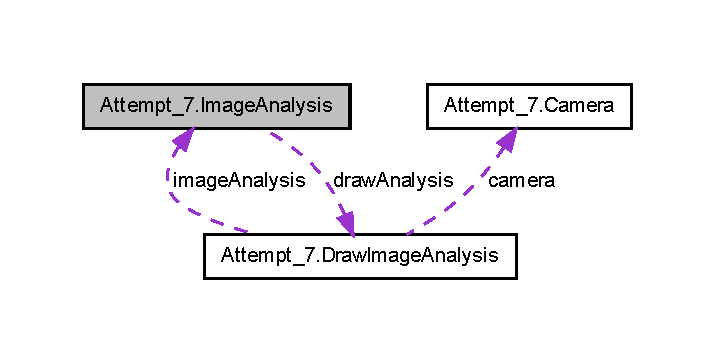
\includegraphics[width=343pt]{class_attempt__7_1_1_image_analysis__coll__graph}
\end{center}
\end{figure}
\subsection*{Public Member Functions}
\begin{DoxyCompactItemize}
\item 
{\bf ImageAnalysis} (Game game, Vector2 screenSize, List$<$ Viewport $>$ viewPortList1)
\begin{DoxyCompactList}\small\item\em Initializes a new instance of the \doxyref{ImageAnalysis}{p.}{class_attempt__7_1_1_image_analysis} class. \item\end{DoxyCompactList}\item 
override void {\bf Initialize} ()
\begin{DoxyCompactList}\small\item\em Called when the class is initialized. Creates many of the arrays and sets many of the values. \item\end{DoxyCompactList}\item 
void {\bf Update1} (GameTime gameTime1)
\begin{DoxyCompactList}\small\item\em Stores the texture from the robot camera in a color array before the texture is disposed. Expicitly called in the \doxyref{SimulationMain}{p.}{class_attempt__7_1_1_simulation_main} Draw method. \item\end{DoxyCompactList}\item 
void {\bf SetRobotCameraView} (Texture2D text)
\begin{DoxyCompactList}\small\item\em Takes a 2D renderTarget/Texture and sets it as the image to analze. Explicitly called in the \doxyref{SimulationMain}{p.}{class_attempt__7_1_1_simulation_main} Draw Method. \item\end{DoxyCompactList}\item 
override void {\bf Update} (GameTime gameTime)
\begin{DoxyCompactList}\small\item\em Calls the analysis methods that actually do all the work. Basically the Main function for the Image Analysis Class. \item\end{DoxyCompactList}\item 
int {\bf GetWhiteCount} ()
\begin{DoxyCompactList}\small\item\em Allows access to the WhiteCount in the image. \item\end{DoxyCompactList}\item 
double[$\,$] {\bf GetHoughInfo} ()
\begin{DoxyCompactList}\small\item\em Gets the houghInfo Array. \item\end{DoxyCompactList}\item 
bool[,] {\bf GetTrueFalseMaptoDraw} ()
\begin{DoxyCompactList}\small\item\em Allows access to the bool map that is to be drawn. \item\end{DoxyCompactList}\item 
string {\bf GetHoughMode} ()
\begin{DoxyCompactList}\small\item\em Gets the Hough mode. 0 = Old, 1 = New. \item\end{DoxyCompactList}\item 
Color[,] {\bf GetColorMapToDraw} ()
\begin{DoxyCompactList}\small\item\em Gets the Color map to be drawn. \item\end{DoxyCompactList}\item 
int {\bf GetTurnIndicator} ()
\begin{DoxyCompactList}\small\item\em Allows the \doxyref{SimulationMain}{p.}{class_attempt__7_1_1_simulation_main} to get the turnIndicator. \item\end{DoxyCompactList}\item 
int {\bf GetSingularitiesNewHough} ()
\begin{DoxyCompactList}\small\item\em Returns the number of times rho=0 in the new hough system. \item\end{DoxyCompactList}\item 
int {\bf GetSingularitesOldHough} ()
\begin{DoxyCompactList}\small\item\em Returns the number of times rho=0 in the Old hough system. \item\end{DoxyCompactList}\item 
Vector3[$\,$] {\bf GetHoughStartandStopVectors} ()
\begin{DoxyCompactList}\small\item\em Gets the array holding information about the hough lines and where to draw them. \item\end{DoxyCompactList}\end{DoxyCompactItemize}
\subsection*{Private Member Functions}
\begin{DoxyCompactItemize}
\item 
Color[,] {\bf TextureTo2DArray} (Texture2D texture, Color[$\,$] colors1D, Color[,] colors2D)
\begin{DoxyCompactList}\small\item\em Takes a texture and makes it into a 2D color array. Passing in the arrays is faster than trying to build it each time. \item\end{DoxyCompactList}\item 
bool[,] {\bf FindWhite} (Color[,] colorArray1)
\begin{DoxyCompactList}\small\item\em Takes a 2D color array and finds the pixels that are \char`\"{}white\char`\"{}. \item\end{DoxyCompactList}\item 
bool[,] {\bf Whiteline} (bool[,] whitemap)
\begin{DoxyCompactList}\small\item\em Determines if white pixels meet the Width threshold to possibly be a line. NOT IN USE RIGHT NOW$\ast$$\ast$$\ast$$\ast$$\ast$$\ast$$\ast$$\ast$$\ast$$\ast$$\ast$$\ast$$\ast$$\ast$$\ast$$\ast$$\ast$$\ast$$\ast$$\ast$. \item\end{DoxyCompactList}\item 
bool[,] {\bf Smooth} (bool[,] original, bool[,] final)
\begin{DoxyCompactList}\small\item\em Takes a truefalse map and for each pixel checks the other pixels around it to see if they are also white. If the number of pixels arround it that are also white is above a threshold then keep that pixel white. Meant to reduce noise in the picture. NOT IN USE RIGHT NOW$\ast$$\ast$$\ast$$\ast$$\ast$$\ast$$\ast$$\ast$$\ast$$\ast$$\ast$$\ast$$\ast$$\ast$$\ast$$\ast$$\ast$$\ast$$\ast$$\ast$. \item\end{DoxyCompactList}\item 
bool[,] {\bf ShowPath} (bool[,] blocked, bool[,] clearPath)
\begin{DoxyCompactList}\small\item\em Find a path through the map to go through and return it as a bool map, also set the turn indicator. Based off the reactiveNavigation from the old robot code. \item\end{DoxyCompactList}\item 
void {\bf FindMaxInAccumArrayOfHough} (short[,] accumToAnalze, short thetaIncrement, short startIndexOfStoringHoughInfoList)
\begin{DoxyCompactList}\small\item\em Finds Max value in Hough. Store information about that max. \item\end{DoxyCompactList}\item 
void {\bf CalculateStartandStopofLine} (double x1, double y1, double slope1, int startIndexforStorageArray)
\begin{DoxyCompactList}\small\item\em Part of the old Hough system. Finds the edge values on the screen of the lines based on the slope and yInt. \item\end{DoxyCompactList}\item 
void {\bf Hough} (bool[,] isLine)
\begin{DoxyCompactList}\small\item\em For each white pixel that might be part of a line, Find all the potiential lines going through it and store each vote for that line in the accumlator's bins. Calls the methods to search through the accumlator to find the bins with the largest values. \item\end{DoxyCompactList}\item 
void {\bf FindAverages} ()
\begin{DoxyCompactList}\small\item\em Find the average theta values. Weigh them according to the rho value of each one. Make a turning desision based off the weighted thetas if turnBytheta is on. \item\end{DoxyCompactList}\item 
short[,] {\bf ClearMaxInAccum} (short[,] accumToChange, int rho, int theta)
\begin{DoxyCompactList}\small\item\em Clears the array arround the maximum. \item\end{DoxyCompactList}\end{DoxyCompactItemize}
\subsection*{Private Attributes}
\begin{DoxyCompactItemize}
\item 
const int {\bf OLD\_\-HOUGH\_\-MODE} = 0
\item 
const int {\bf New\_\-HOUGH\_\-MODE} = 1
\item 
const short {\bf NumberofLinesToFind} = 2
\begin{DoxyCompactList}\small\item\em Number of lines the hough transform should find. \item\end{DoxyCompactList}\item 
const int {\bf AccumLength} = 600
\begin{DoxyCompactList}\small\item\em Size of the Acuumlator's lenght. Must be able to fit the largest posible value of rho. Max rho = Sqrt( ScreenHeight$^\wedge$2+ (ScreenWidth/2)$^\wedge$2), because the origin is the bottom center and the max rho is top left or right. \item\end{DoxyCompactList}\item 
const int {\bf AccumLengthOld} = 810
\begin{DoxyCompactList}\small\item\em lenght of the hold hough accumulator \item\end{DoxyCompactList}\item 
const short {\bf ThetaIncrement} = 3
\begin{DoxyCompactList}\small\item\em How big the steps are for a potiential theta. In degreees. Large values reduce computation but less acurate. \item\end{DoxyCompactList}\item 
const short {\bf RhoIncrement} = 6
\begin{DoxyCompactList}\small\item\em How big the steps are for a potiential rho values. Large values reduce computation but less acurate. \item\end{DoxyCompactList}\item 
const short {\bf UpdateSquareDimForDrawing} = 2
\begin{DoxyCompactList}\small\item\em Inorder to make computations go faster, not every pixels is anylzed every time. 1 out of This value squared is analzed each pass. \item\end{DoxyCompactList}\item 
const short {\bf UpdateSquareDimForAnalysis} = 2
\begin{DoxyCompactList}\small\item\em Inorder to make drawing go faster, not every pixels is updated every time. 1 out of This value squared is updated each pass. \item\end{DoxyCompactList}\item 
const int {\bf ClearArroundMaxDegree} = 5
\begin{DoxyCompactList}\small\item\em Number of degrees around a maximum to clear around before searching the Accumulator again. \item\end{DoxyCompactList}\item 
const int {\bf ClearArroundMaxRho} = 8
\begin{DoxyCompactList}\small\item\em Number of rho values around a maximum to clear around before searching the Accumulator again. \item\end{DoxyCompactList}\item 
const int {\bf SmoothSearchSize} = 4
\begin{DoxyCompactList}\small\item\em Used by the smooth method. Dimension of Number of pixels to look around for the smooth function. This (values$\ast$2)$^\wedge$2 = number of pixels checked. \item\end{DoxyCompactList}\item 
int {\bf currentMode} = 0
\begin{DoxyCompactList}\small\item\em If 0 then Old mode (top left origin), if 1 then New Hough mode( bottom Center). \item\end{DoxyCompactList}\item 
bool {\bf turnIndicatorisTheta} = false
\begin{DoxyCompactList}\small\item\em If true then steering desisions will be based off the theta's of the hough transform. \item\end{DoxyCompactList}\item 
Texture2D {\bf robotCameraView}
\begin{DoxyCompactList}\small\item\em Texture object that represents the robot camera's current view. \item\end{DoxyCompactList}\item 
bool[,] {\bf trueFalseMap}
\begin{DoxyCompactList}\small\item\em TrueFalse maps used for marking pixels either \char`\"{}good\char`\"{} or \char`\"{}bad\char`\"{}. \item\end{DoxyCompactList}\item 
bool[,] {\bf trueFalseMapB}
\item 
bool[,] {\bf trueFalseMapC}
\item 
int {\bf screenWidth}
\begin{DoxyCompactList}\small\item\em Screen Width of the image to analze. \item\end{DoxyCompactList}\item 
int {\bf screenHeight}
\begin{DoxyCompactList}\small\item\em Screen Height of the image to analze. \item\end{DoxyCompactList}\item 
int {\bf turnIndication} = 0
\begin{DoxyCompactList}\small\item\em The turn indicator measures measures how much the analysis things the robot should go right or left. Right = positive. Left = negative. \item\end{DoxyCompactList}\item 
double[$\,$] {\bf houghInfo}
\begin{DoxyCompactList}\small\item\em Stores information about lines from the hough transform. each polarRho we want to find = 7 more values to store 0=slope, 1= yInt, 2=Rho, 3=Theta, 4=Xvalue, 5=Yvalue, 6= size of the bin, 7= xTransformed value 8= yTransformedValue, 9 = distance to line Algorithm, 10= angle to line Algorithm 5 more ending values for the averages. \item\end{DoxyCompactList}\item 
Vector3[$\,$] {\bf houghLineStartandStopVectors}
\begin{DoxyCompactList}\small\item\em Stores vector3 locations of the beginning and end points of two lines on the screen. Was part of the old Hough system, but potientially still useful, so has not deleted. 0 = start location of line, 1 = end location ofline. \item\end{DoxyCompactList}\item 
Color[,] {\bf colorArray}
\begin{DoxyCompactList}\small\item\em Color Array 2D from the robot camera that is analzed. \item\end{DoxyCompactList}\item 
Color[$\,$] {\bf colorArray1D}
\begin{DoxyCompactList}\small\item\em Color Array 2D from the robot camera that is analzed. Can't extract informatino directly from the robot view Texture to 2D. But have to go through 1D array. \item\end{DoxyCompactList}\item 
short {\bf count1A} = 0
\begin{DoxyCompactList}\small\item\em These values are the incremented numbers used in the giant double \char`\"{}for-\/loops\char`\"{}. The \char`\"{}1\char`\"{} values are the for the first \char`\"{}for-\/loop\char`\"{}. \item\end{DoxyCompactList}\item 
short {\bf count1B} = 1
\item 
short {\bf count1C} = 0
\item 
short {\bf count1D} = 1
\item 
short {\bf count1E} = 0
\item 
short {\bf count2A} = 0
\begin{DoxyCompactList}\small\item\em These values are the incremented numbers used in the giant double \char`\"{}for-\/loops\char`\"{}. The \char`\"{}2\char`\"{} values are the for the second \char`\"{}for-\/loop\char`\"{}. \item\end{DoxyCompactList}\item 
short {\bf count2B} = 0
\item 
short {\bf count2C} = 0
\item 
short {\bf count2E} = 0
\item 
int[$\,$] {\bf middleValues}
\begin{DoxyCompactList}\small\item\em An array of the middle clear pixels for each row. The length of the array is the number of rows = this.screenHeight. \item\end{DoxyCompactList}\item 
int {\bf totalWhiteCnt} = 0
\begin{DoxyCompactList}\small\item\em Number of white pixels the \char`\"{}FindWhite\char`\"{} found. \item\end{DoxyCompactList}\item 
short[,] {\bf accum2}
\begin{DoxyCompactList}\small\item\em The accumlator for the hough values. Each position is a hough Bin. Each bin represents a line in Cartessian cordinates. The Accumlator is basically in polar cordinates. Theta,rho. \item\end{DoxyCompactList}\item 
short[,] {\bf accum1}
\item 
int {\bf cntThreshold} = 15
\begin{DoxyCompactList}\small\item\em Used by the smooth method. How many pixels must also be white in the area around a white pixel for it to be counted white. \item\end{DoxyCompactList}\item 
int {\bf redGood}
\begin{DoxyCompactList}\small\item\em On a scale of 0-\/255 how high does a pixel RGB value have to be before being declared white. \item\end{DoxyCompactList}\item 
int {\bf blueGood}
\item 
int {\bf greenGood}
\item 
int {\bf whiteParam} = 150
\begin{DoxyCompactList}\small\item\em Sets red\_\-good, blue\_\-good, green\_\-good to this value. \item\end{DoxyCompactList}\item 
{\bf DrawImageAnalysis} {\bf drawAnalysis}
\begin{DoxyCompactList}\small\item\em The drawingImageAnalysis class handles the vertex information the shows what the robot is thinking. \item\end{DoxyCompactList}\item 
int {\bf countOfNewHoughSingularities} = 0
\item 
int {\bf countofOldHoughSingularities} = 0
\end{DoxyCompactItemize}


\subsection{Detailed Description}
It was easier to redure 640$\ast$480 small triangles and view then from a distance than to put a texture on the GPU So there is a camera to view the triangels. The class only analzes a small fraction of the pixels each time through the game loop inorder to keep the speed high. Many of the methods have loops that cause them to only look at every X pixel each time through and then the next time through a different set. Basically it functions like a giant double \char`\"{}for\char`\"{} loop. The Image Analysis Class does the image processing of the robot view. 

Definition at line 32 of file ImageAnalysis2.cs.



\subsection{Constructor \& Destructor Documentation}
\index{Attempt\_\-7::ImageAnalysis@{Attempt\_\-7::ImageAnalysis}!ImageAnalysis@{ImageAnalysis}}
\index{ImageAnalysis@{ImageAnalysis}!Attempt_7::ImageAnalysis@{Attempt\_\-7::ImageAnalysis}}
\subsubsection[{ImageAnalysis}]{\setlength{\rightskip}{0pt plus 5cm}Attempt\_\-7.ImageAnalysis.ImageAnalysis (
\begin{DoxyParamCaption}
\item[{Game}]{game, }
\item[{Vector2}]{screenSize, }
\item[{List$<$ Viewport $>$}]{viewPortList1}
\end{DoxyParamCaption}
)}\label{class_attempt__7_1_1_image_analysis_a372086fbe7753711c79fb65694e74b8b}


Initializes a new instance of the \doxyref{ImageAnalysis}{p.}{class_attempt__7_1_1_image_analysis} class. 


\begin{DoxyParams}{Parameters}
{\em game} & The game associated with the class\\
\hline
{\em screenSize} & The size of the sceen to analze\\
\hline
{\em viewPortList1} & A list of the view ports\\
\hline
\end{DoxyParams}


Definition at line 203 of file ImageAnalysis2.cs.


\begin{DoxyCode}
            : base(game)
        {
            this.screenWidth = (int)screenSize.X;
            this.screenHeight = (int)screenSize.Y;

            // Creates the image drawing analysis object.
            this.drawAnalysis = new DrawImageAnalysis(game, this.screenWidth, thi
      s.screenHeight, UpdateSquareDimForDrawing, UpdateSquareDimForAnalysis, 
      NumberofLinesToFind, ThetaIncrement, RhoIncrement, viewPortList1, this);
            this.drawAnalysis.DrawOrder = game.Components.Count;
            Game.Components.Add(this.drawAnalysis);
        }
\end{DoxyCode}


\subsection{Member Function Documentation}
\index{Attempt\_\-7::ImageAnalysis@{Attempt\_\-7::ImageAnalysis}!CalculateStartandStopofLine@{CalculateStartandStopofLine}}
\index{CalculateStartandStopofLine@{CalculateStartandStopofLine}!Attempt_7::ImageAnalysis@{Attempt\_\-7::ImageAnalysis}}
\subsubsection[{CalculateStartandStopofLine}]{\setlength{\rightskip}{0pt plus 5cm}void Attempt\_\-7.ImageAnalysis.CalculateStartandStopofLine (
\begin{DoxyParamCaption}
\item[{double}]{x1, }
\item[{double}]{y1, }
\item[{double}]{slope1, }
\item[{int}]{startIndexforStorageArray}
\end{DoxyParamCaption}
)\hspace{0.3cm}{\ttfamily  [private]}}\label{class_attempt__7_1_1_image_analysis_a327ee82eeb29ad6f4060bb4a9a21d7d8}


Part of the old Hough system. Finds the edge values on the screen of the lines based on the slope and yInt. 


\begin{DoxyParams}{Parameters}
{\em slope1} & Slope of the line\\
\hline
{\em yintercept1} & YIntercept of the line\\
\hline
{\em startIndexforStorageArray} & Where to store the information in the storage array\\
\hline
\end{DoxyParams}


Definition at line 709 of file ImageAnalysis2.cs.


\begin{DoxyCode}
        {
            int startX = 0;
            int startY = 0;
            int endX = 0;
            int endY = 0;
            int yIntReal = 0;
            double slopeReal = 0;

            if (this.currentMode == New_HOUGH_MODE)
            {
                slopeReal = -1 / slope1; // Slope of the actual line-- not the sl
      ope of the line perpendicular (which is what the hough found)
                yIntReal = (int)(y1 - (slopeReal * (x1 + this.screenWidth / 2)));
       // y-intercept of the actual line-- not the slope of the line perpendicular (whi
      ch is what the hough found)

                // So far all the calculations assume origin is in bottom center.
       Now based off that information find the cordinates of where to start and stop
                // the hough lines in screen cordinates. Down is positive y in sc
      reen cordinates.             
                // Left Side
                if (yIntReal >= 0 && yIntReal < this.screenHeight)
                {
                    startX = 0;
                    startY = this.screenHeight - yIntReal;                    
                }
                else if (yIntReal <= 0)
                {                    
                    startX = -(int)(yIntReal / slopeReal);
                    startY = this.screenHeight;
                }
                else if (yIntReal > this.screenHeight)
                {
                    startX = (int)((this.screenHeight - yIntReal) / slopeReal);
                    startY = 0;
                }

                // Find the end cordinates of the line.
                // Right Side          
                int yright = (int)((slopeReal * this.screenWidth) + yIntReal);

                if (yright > 0 && yright < this.screenHeight)
                {                    
                    endX = this.screenWidth;
                    endY = this.screenHeight - yright;
                }
                else if (yright < 0)
                {
                    endX = (int)(-yIntReal / slopeReal);
                    endY = this.screenHeight;
                }
                else

                    if (yright > this.screenHeight)
                    {
                        endX = (int)((this.screenHeight - yIntReal) / slopeReal);
      
                        endY = 0;
                    }
            }

            if (this.currentMode == OLD_HOUGH_MODE)
            {
                // remember that origin is top left corner and down is positive y
      
                slopeReal = -1 / -slope1;
                yIntReal = (int)(-y1 - (slopeReal * x1));

                if (yIntReal >= 0)
                {
                    startX = (int)(-yIntReal / slopeReal);
                    startY = 0;
                }

                if (yIntReal <= 0 && yIntReal > -this.screenHeight)
                {
                    startX = 0;
                    startY = -(int)yIntReal;
                }

                if (yIntReal < -this.screenHeight)
                {
                    startX = (int)((-this.screenHeight - yIntReal) / slopeReal);
                    startY = this.screenHeight;
                }

                // Find the end cordinates of the line.
                // Right Side          
                int yright = (int)((slopeReal * this.screenWidth) + yIntReal);

                if (yright > 0)
                {
                    endX = (int)(-yIntReal / slopeReal);
                    endY = 0;
                }

                if (yright < 0 && yright > -this.screenHeight)
                {
                    endX = this.screenWidth;
                    endY = -yright;
                }

                if (yright < -this.screenHeight)
                {
                    endX = (int)((-this.screenHeight - yIntReal) / slopeReal);
                    endY = this.screenHeight;
                }

            }

            // Store the Line information in the array 'houghLineStartandStopVect
      ors' starting at the value 'startIndexforStorageArray'
            this.houghLineStartandStopVectors[startIndexforStorageArray + 0] = ne
      w Vector3(startX, startY, 0);
            this.houghLineStartandStopVectors[startIndexforStorageArray + 1] = ne
      w Vector3(endX, endY, 0);
        }
\end{DoxyCode}


Here is the caller graph for this function:\nopagebreak
\begin{figure}[H]
\begin{center}
\leavevmode
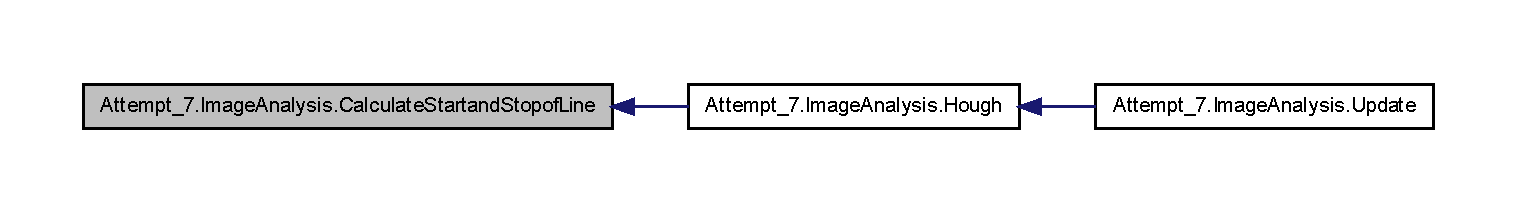
\includegraphics[width=400pt]{class_attempt__7_1_1_image_analysis_a327ee82eeb29ad6f4060bb4a9a21d7d8_icgraph}
\end{center}
\end{figure}


\index{Attempt\_\-7::ImageAnalysis@{Attempt\_\-7::ImageAnalysis}!ClearMaxInAccum@{ClearMaxInAccum}}
\index{ClearMaxInAccum@{ClearMaxInAccum}!Attempt_7::ImageAnalysis@{Attempt\_\-7::ImageAnalysis}}
\subsubsection[{ClearMaxInAccum}]{\setlength{\rightskip}{0pt plus 5cm}short [,] Attempt\_\-7.ImageAnalysis.ClearMaxInAccum (
\begin{DoxyParamCaption}
\item[{short}]{accumToChange[,], }
\item[{int}]{rho, }
\item[{int}]{theta}
\end{DoxyParamCaption}
)\hspace{0.3cm}{\ttfamily  [private]}}\label{class_attempt__7_1_1_image_analysis_a00bfc4bb52ece15ba645b81fb3ca3f2b}


Clears the array arround the maximum. 


\begin{DoxyParams}{Parameters}
{\em accumToChange} & The accumulator to clear around\\
\hline
{\em rho} & the rho value to clear around\\
\hline
{\em theta} & the theta value to clear around\\
\hline
\end{DoxyParams}
\begin{DoxyReturn}{Returns}
the accumulator array that is cleared around
\end{DoxyReturn}


Definition at line 982 of file ImageAnalysis2.cs.


\begin{DoxyCode}
        {
            rho = rho / RhoIncrement;
            theta = theta / ThetaIncrement;

            int accumDim1 = accumToChange.GetLength(0); // Get the size accum Arr
      ay
            int accumDim2 = accumToChange.GetLength(1);

            // Clear the one with the most votes
            for (int degree = -ClearArroundMaxDegree / ThetaIncrement; degree < 
      ClearArroundMaxDegree / ThetaIncrement; degree++)
            {
                for (int phi = -ClearArroundMaxRho / RhoIncrement; phi < 
      ClearArroundMaxRho / RhoIncrement; phi++)
                {
                    int thetaprime = (theta + degree) % accumDim1;
                    int rhoprime = (rho + phi) % accumDim2;
                    if (thetaprime > 0 && thetaprime < accumDim1 && rhoprime > 0 
      && rhoprime < accumDim2)
                    {
                        accumToChange[thetaprime, rhoprime] = 0;
                    }
                }
            }

            return accumToChange;
        }
\end{DoxyCode}


Here is the caller graph for this function:\nopagebreak
\begin{figure}[H]
\begin{center}
\leavevmode
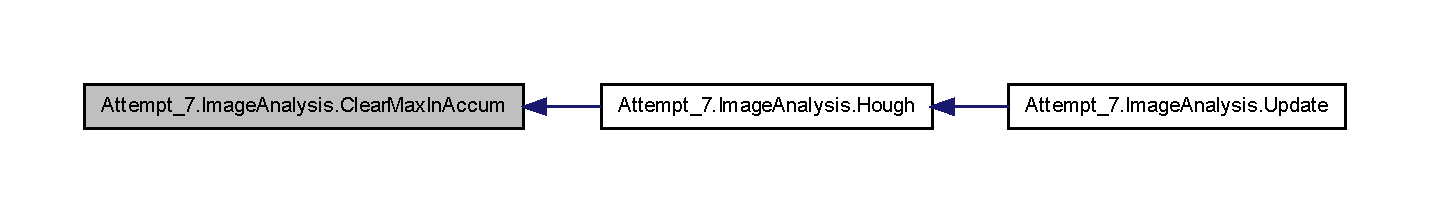
\includegraphics[width=400pt]{class_attempt__7_1_1_image_analysis_a00bfc4bb52ece15ba645b81fb3ca3f2b_icgraph}
\end{center}
\end{figure}


\index{Attempt\_\-7::ImageAnalysis@{Attempt\_\-7::ImageAnalysis}!FindAverages@{FindAverages}}
\index{FindAverages@{FindAverages}!Attempt_7::ImageAnalysis@{Attempt\_\-7::ImageAnalysis}}
\subsubsection[{FindAverages}]{\setlength{\rightskip}{0pt plus 5cm}void Attempt\_\-7.ImageAnalysis.FindAverages (
\begin{DoxyParamCaption}
{}
\end{DoxyParamCaption}
)\hspace{0.3cm}{\ttfamily  [private]}}\label{class_attempt__7_1_1_image_analysis_aa983bdc246185a5a41414e1db84534dd}


Find the average theta values. Weigh them according to the rho value of each one. Make a turning desision based off the weighted thetas if turnBytheta is on. 



Definition at line 941 of file ImageAnalysis2.cs.


\begin{DoxyCode}
        {
            int thetaSum = 0;
            int rhoSum = 0;
            int count = 0;
            int rho = -1;
            int theta = -1;
            int binSize = 0;
            int turn = -1;

            for (int i = 0; i < NumberofLinesToFind; i++)
            {
                // If the rho or theta are the same as the last one, then don't c
      ount it. 
                if (this.houghInfo[((i * 11) + 4)] != rho && this.houghInfo[((i *
       11) + 5)] != theta && this.houghInfo[((i * 11) + 6)] * 1.5 > binSize)
                {
                    rho = (int)this.houghInfo[((i * 11) + 2)]; // Sum the rhos
                    theta = (int)this.houghInfo[((i * 11) + 3)]; // Sum the theta
      s
                    binSize = (int)this.houghInfo[((i * 11) + 4)]; // Get bin siz
      e
                    rhoSum += rho;
                    thetaSum += theta;
                    turn += (int)((theta - 90) * (double)((i / NumberofLinesToFin
      d) * (577 - rho) / 500));
                    count++;
                }
            }

            int averageTheta = thetaSum / count;
            this.houghInfo[NumberofLinesToFind * 11] = averageTheta; // Compute a
      nd store the averages
            this.houghInfo[(NumberofLinesToFind * 11) + 1] = rhoSum / count;
            if (this.turnIndicatorisTheta == true)
            {
                this.turnIndication = turn;
            }
        }
\end{DoxyCode}


Here is the caller graph for this function:\nopagebreak
\begin{figure}[H]
\begin{center}
\leavevmode
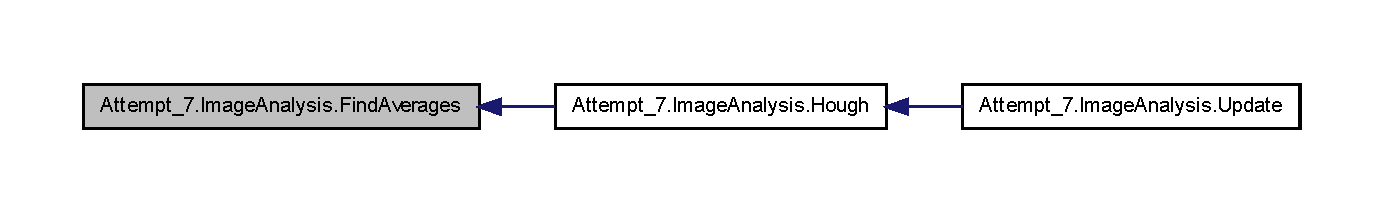
\includegraphics[width=400pt]{class_attempt__7_1_1_image_analysis_aa983bdc246185a5a41414e1db84534dd_icgraph}
\end{center}
\end{figure}


\index{Attempt\_\-7::ImageAnalysis@{Attempt\_\-7::ImageAnalysis}!FindMaxInAccumArrayOfHough@{FindMaxInAccumArrayOfHough}}
\index{FindMaxInAccumArrayOfHough@{FindMaxInAccumArrayOfHough}!Attempt_7::ImageAnalysis@{Attempt\_\-7::ImageAnalysis}}
\subsubsection[{FindMaxInAccumArrayOfHough}]{\setlength{\rightskip}{0pt plus 5cm}void Attempt\_\-7.ImageAnalysis.FindMaxInAccumArrayOfHough (
\begin{DoxyParamCaption}
\item[{short}]{accumToAnalze[,], }
\item[{short}]{thetaIncrement, }
\item[{short}]{startIndexOfStoringHoughInfoList}
\end{DoxyParamCaption}
)\hspace{0.3cm}{\ttfamily  [private]}}\label{class_attempt__7_1_1_image_analysis_a74a456e2880a858c96a7d8802250c504}


Finds Max value in Hough. Store information about that max. 


\begin{DoxyParams}{Parameters}
{\em accumToAnalze} & The accumlator of bins we want to search\\
\hline
{\em thetaIncrement} & How large is the quantitization of the theta values. \\
\hline
{\em startIndexOfStoringHoughInfoList} & What value in the Array 'HoughInfo' should we start storing information.\\
\hline
\end{DoxyParams}


\{(x$^\wedge$3 -\/ b x y + a y$^\wedge$2 + x y$^\wedge$2)/(x$^\wedge$2 + y$^\wedge$2), x$^\wedge$2/y + y -\/ (x (x$^\wedge$3 -\/ b x y + a y$^\wedge$2 + x y$^\wedge$2))/(y (x$^\wedge$2 + y$^\wedge$2))\} 



Definition at line 599 of file ImageAnalysis2.cs.


\begin{DoxyCode}
        {
            int maxTheta = 1;
            int maxRho = 1;
            int maxAccum = 1;
            int accumDim1 = accumToAnalze.GetLength(0);
            int accumDim2 = accumToAnalze.GetLength(1);

            // Run through to find cell with most votes
            for (int s = 0; s < accumDim1; s++)
            {
                for (int t = 0; t < accumDim2; t++)
                {
                    if (accumToAnalze[s, t] > maxAccum)
                    {
                        maxTheta = s;
                        maxRho = t;
                        maxAccum = accumToAnalze[s, t];
                    }
                }
            }

            double slope1 = 1;
            int yintercept1 = 0;
            double x1 = 0;
            double y1 = 0;

            if (this.currentMode == New_HOUGH_MODE)
            {
                maxTheta *= thetaIncrement; // Scale the Theta back to real size.
      
                maxRho = maxRho * RhoIncrement; // Scale the Rho back to real siz
      e.
                x1 = (int)(maxRho * Math.Cos(MathHelper.ToRadians(maxTheta))); //
       Find the x Point corresponding the theta, rho
                y1 = (int)(maxRho * Math.Sin(MathHelper.ToRadians(maxTheta))); //
       Find the y Point corresponding the theta, rho               

                if (x1 == 0)
                {
                    x1 = 0.00001; // don't divide by zero
                }
                slope1 = Math.Round(Math.Tan(MathHelper.ToRadians(maxTheta)), 2);
       // Calculating the slope and round to 2 digits.                
                yintercept1 = (int)(y1 - (slope1 * x1));

                // Store the information found about the line in the 'this.houghI
      nfo' array starting at the value 'StartIndexOfStoringHoughInfoList'
                this.houghInfo[startIndexOfStoringHoughInfoList + 0] = slope1;
                this.houghInfo[startIndexOfStoringHoughInfoList + 1] = yintercept
      1;
                this.houghInfo[startIndexOfStoringHoughInfoList + 2] = maxRho;
                this.houghInfo[startIndexOfStoringHoughInfoList + 3] = maxTheta;
                this.houghInfo[startIndexOfStoringHoughInfoList + 4] = x1;
                this.houghInfo[startIndexOfStoringHoughInfoList + 5] = y1;
                this.houghInfo[startIndexOfStoringHoughInfoList + 6] = maxAccum;
            }

            if (this.currentMode == OLD_HOUGH_MODE)
            {
                maxTheta = (thetaIncrement * maxTheta) - 180; // Scale the Theta 
      back to real size.
                maxRho = maxRho * RhoIncrement; // Scale the Rho back to real siz
      e.
                x1 = (int)(maxRho * Math.Cos(MathHelper.ToRadians(maxTheta))); //
       Find the x Point corresponding the theta, rho
                y1 = (int)(maxRho * Math.Sin(MathHelper.ToRadians(maxTheta))); //
       Find the y Point corresponding the theta, rho               

                if (x1 == 0)
                {
                    x1 = 0.00001; // don't divide by zero
                }
                slope1 = Math.Round(Math.Tan(MathHelper.ToRadians(maxTheta)), 2);
       // Calculating the slope and round to 2 digits.                
                yintercept1 = (int)(y1 - (slope1 * x1));


                int distance = 0;
                int angle = 0;
                int a = this.screenWidth / 2;
                int b = this.screenHeight;

                double xTransformed = (int)((Math.Pow(x1, 3) - b * x1 * y1 + a * 
      Math.Pow(y1, 2) + x1 * Math.Pow(y1, 2)) / (Math.Pow(x1, 2) + Math.Pow(y1, 2)));
                double yTransformed = (int)(Math.Pow(x1, 2) / y1 + y1 - (x1 * (Ma
      th.Pow(x1, 3) - b * x1 * y1 + a * Math.Pow(y1, 2) + x1 * Math.Pow(y1, 2))) / (y1 
      * (Math.Pow(x1, 2) + Math.Pow(y1, 2))));

                distance = (int)Math.Sqrt(Math.Pow(xTransformed - a, 2) + Math.Po
      w(b - yTransformed, 2));
                angle = (int)MathHelper.ToDegrees((float)Math.Atan((b - yTransfor
      med) / (xTransformed - a)));

                if (angle < 0)
                {
                    angle += 180;
                }

                // Store the information found about the line in the 'this.houghI
      nfo' array starting at the value 'StartIndexOfStoringHoughInfoList'
                this.houghInfo[startIndexOfStoringHoughInfoList + 0] = slope1;
                this.houghInfo[startIndexOfStoringHoughInfoList + 1] = yintercept
      1;
                this.houghInfo[startIndexOfStoringHoughInfoList + 2] = maxRho;
                this.houghInfo[startIndexOfStoringHoughInfoList + 3] = maxTheta +
       180; // Stay in the range of the array. 
                this.houghInfo[startIndexOfStoringHoughInfoList + 4] = x1;
                this.houghInfo[startIndexOfStoringHoughInfoList + 5] = y1;
                this.houghInfo[startIndexOfStoringHoughInfoList + 6] = maxAccum;
                this.houghInfo[startIndexOfStoringHoughInfoList + 7] = xTransform
      ed;
                this.houghInfo[startIndexOfStoringHoughInfoList + 8] = yTransform
      ed;
                this.houghInfo[startIndexOfStoringHoughInfoList + 9] = distance; 
      // distance to line. 
                this.houghInfo[startIndexOfStoringHoughInfoList + 10] = angle; //
       angle to line. 
            }

        }
\end{DoxyCode}


Here is the caller graph for this function:\nopagebreak
\begin{figure}[H]
\begin{center}
\leavevmode
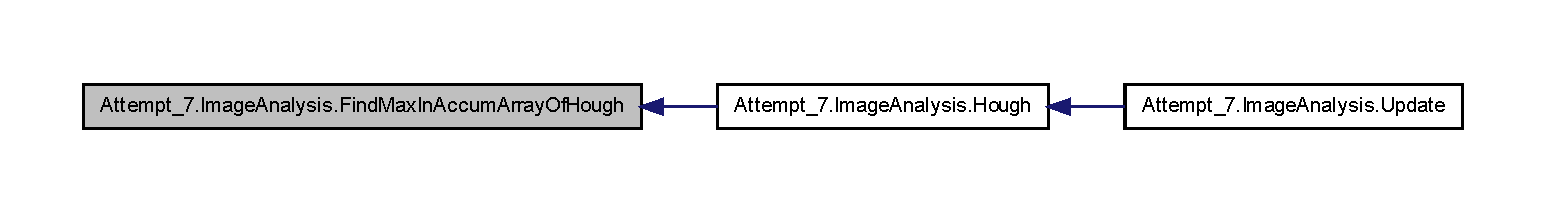
\includegraphics[width=400pt]{class_attempt__7_1_1_image_analysis_a74a456e2880a858c96a7d8802250c504_icgraph}
\end{center}
\end{figure}


\index{Attempt\_\-7::ImageAnalysis@{Attempt\_\-7::ImageAnalysis}!FindWhite@{FindWhite}}
\index{FindWhite@{FindWhite}!Attempt_7::ImageAnalysis@{Attempt\_\-7::ImageAnalysis}}
\subsubsection[{FindWhite}]{\setlength{\rightskip}{0pt plus 5cm}bool [,] Attempt\_\-7.ImageAnalysis.FindWhite (
\begin{DoxyParamCaption}
\item[{Color}]{colorArray1[,]}
\end{DoxyParamCaption}
)\hspace{0.3cm}{\ttfamily  [private]}}\label{class_attempt__7_1_1_image_analysis_a9418e8e0a6868d294d27b97cadf6d958}


Takes a 2D color array and finds the pixels that are \char`\"{}white\char`\"{}. 


\begin{DoxyParams}{Parameters}
{\em colorArray1} & The color array to find white in.\\
\hline
\end{DoxyParams}
\begin{DoxyReturn}{Returns}
The TrueFalse bool map of white pixels. True = white, False = not white. 
\end{DoxyReturn}


Definition at line 409 of file ImageAnalysis2.cs.


\begin{DoxyCode}
        {
            // True = bad, False = good.
            this.totalWhiteCnt = 0;
            int i, j;
            bool[,] trueFalseMap = new bool[colorArray1.GetLength(0), colorArray1
      .GetLength(1)]; // Create the bool map.

            for (i = 0; i < this.screenWidth; ++i)
            {
                for (j = 0; j < this.screenHeight; ++j)
                {
                    // If above the thresholds. 
                    if ((colorArray1[i, j].R > this.redGood)
                        && (colorArray1[i, j].G > this.greenGood)
                        && (colorArray1[i, j].B > this.blueGood))
                    {
                        trueFalseMap[i, j] = true;
                        this.totalWhiteCnt++;
                    }
                    else
                    {
                        trueFalseMap[i, j] = false;
                    }
                }
            }

            return trueFalseMap;
        }
\end{DoxyCode}


Here is the caller graph for this function:\nopagebreak
\begin{figure}[H]
\begin{center}
\leavevmode
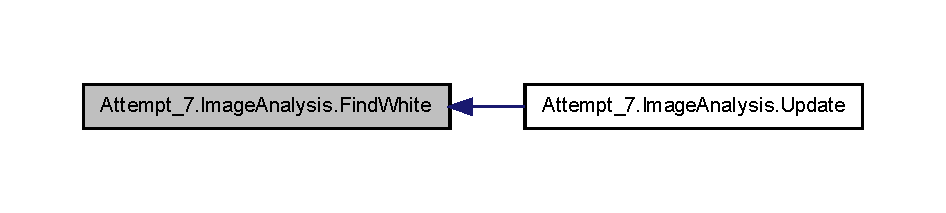
\includegraphics[width=400pt]{class_attempt__7_1_1_image_analysis_a9418e8e0a6868d294d27b97cadf6d958_icgraph}
\end{center}
\end{figure}


\index{Attempt\_\-7::ImageAnalysis@{Attempt\_\-7::ImageAnalysis}!GetColorMapToDraw@{GetColorMapToDraw}}
\index{GetColorMapToDraw@{GetColorMapToDraw}!Attempt_7::ImageAnalysis@{Attempt\_\-7::ImageAnalysis}}
\subsubsection[{GetColorMapToDraw}]{\setlength{\rightskip}{0pt plus 5cm}Color [,] Attempt\_\-7.ImageAnalysis.GetColorMapToDraw (
\begin{DoxyParamCaption}
{}
\end{DoxyParamCaption}
)}\label{class_attempt__7_1_1_image_analysis_ab8604cecb2f620a88298bccc48a4436d}


Gets the Color map to be drawn. 

\begin{DoxyReturn}{Returns}
Color map
\end{DoxyReturn}


Definition at line 342 of file ImageAnalysis2.cs.


\begin{DoxyCode}
        {
            return this.colorArray;
        }
\end{DoxyCode}
\index{Attempt\_\-7::ImageAnalysis@{Attempt\_\-7::ImageAnalysis}!GetHoughInfo@{GetHoughInfo}}
\index{GetHoughInfo@{GetHoughInfo}!Attempt_7::ImageAnalysis@{Attempt\_\-7::ImageAnalysis}}
\subsubsection[{GetHoughInfo}]{\setlength{\rightskip}{0pt plus 5cm}double [$\,$] Attempt\_\-7.ImageAnalysis.GetHoughInfo (
\begin{DoxyParamCaption}
{}
\end{DoxyParamCaption}
)}\label{class_attempt__7_1_1_image_analysis_a897a0f80fbf65670828c8a1a1db13d97}


Gets the houghInfo Array. 

\begin{DoxyReturn}{Returns}
houghInfo Array
\end{DoxyReturn}


Definition at line 304 of file ImageAnalysis2.cs.


\begin{DoxyCode}
        {
            return this.houghInfo;
        }
\end{DoxyCode}


Here is the caller graph for this function:\nopagebreak
\begin{figure}[H]
\begin{center}
\leavevmode
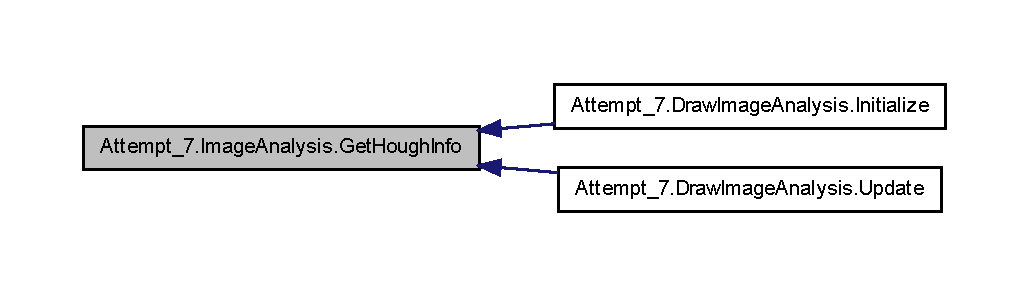
\includegraphics[width=400pt]{class_attempt__7_1_1_image_analysis_a897a0f80fbf65670828c8a1a1db13d97_icgraph}
\end{center}
\end{figure}


\index{Attempt\_\-7::ImageAnalysis@{Attempt\_\-7::ImageAnalysis}!GetHoughMode@{GetHoughMode}}
\index{GetHoughMode@{GetHoughMode}!Attempt_7::ImageAnalysis@{Attempt\_\-7::ImageAnalysis}}
\subsubsection[{GetHoughMode}]{\setlength{\rightskip}{0pt plus 5cm}string Attempt\_\-7.ImageAnalysis.GetHoughMode (
\begin{DoxyParamCaption}
{}
\end{DoxyParamCaption}
)}\label{class_attempt__7_1_1_image_analysis_ae14af27b7aaa3d4a1006af2a56ab14d1}


Gets the Hough mode. 0 = Old, 1 = New. 

\begin{DoxyReturn}{Returns}
\char`\"{}Old\char`\"{} if in the old mode, \char`\"{}New\char`\"{} if in the new mode
\end{DoxyReturn}


Definition at line 322 of file ImageAnalysis2.cs.


\begin{DoxyCode}
        {
            string mode = string.Empty;

            if (this.currentMode == 0)
            {
                mode = "Old";
            }
            else
            {
                mode = "New";
            }

            return mode;
        }
\end{DoxyCode}


Here is the caller graph for this function:
\nopagebreak
\begin{figure}[H]
\begin{center}
\leavevmode
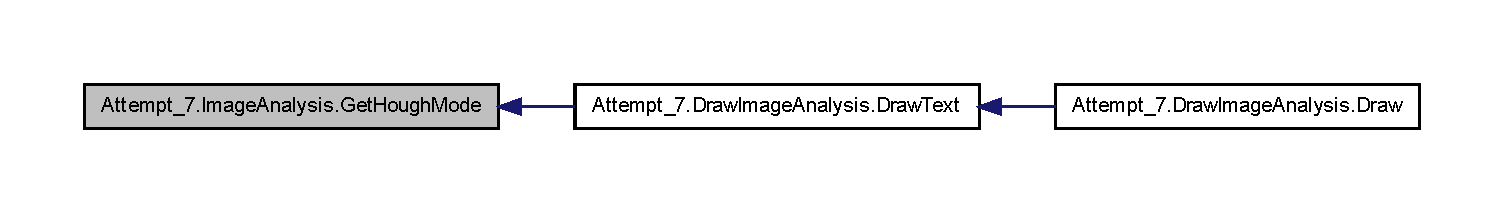
\includegraphics[width=400pt]{class_attempt__7_1_1_image_analysis_ae14af27b7aaa3d4a1006af2a56ab14d1_icgraph}
\end{center}
\end{figure}


\index{Attempt\_\-7::ImageAnalysis@{Attempt\_\-7::ImageAnalysis}!GetHoughStartandStopVectors@{GetHoughStartandStopVectors}}
\index{GetHoughStartandStopVectors@{GetHoughStartandStopVectors}!Attempt_7::ImageAnalysis@{Attempt\_\-7::ImageAnalysis}}
\subsubsection[{GetHoughStartandStopVectors}]{\setlength{\rightskip}{0pt plus 5cm}Vector3 [$\,$] Attempt\_\-7.ImageAnalysis.GetHoughStartandStopVectors (
\begin{DoxyParamCaption}
{}
\end{DoxyParamCaption}
)}\label{class_attempt__7_1_1_image_analysis_a3c35b4a6a6a1e4464fc79772caa612cf}


Gets the array holding information about the hough lines and where to draw them. 

\begin{DoxyReturn}{Returns}
Array of Vector3 with the locations of where to start and stop hough lines
\end{DoxyReturn}


Definition at line 378 of file ImageAnalysis2.cs.


\begin{DoxyCode}
        {
            return this.houghLineStartandStopVectors;
        }
\end{DoxyCode}


Here is the caller graph for this function:\nopagebreak
\begin{figure}[H]
\begin{center}
\leavevmode
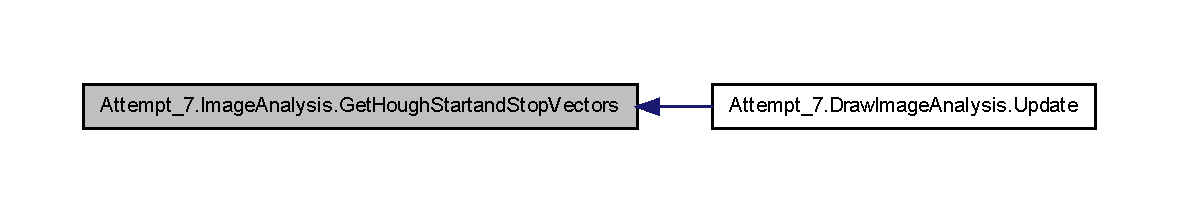
\includegraphics[width=400pt]{class_attempt__7_1_1_image_analysis_a3c35b4a6a6a1e4464fc79772caa612cf_icgraph}
\end{center}
\end{figure}


\index{Attempt\_\-7::ImageAnalysis@{Attempt\_\-7::ImageAnalysis}!GetSingularitesOldHough@{GetSingularitesOldHough}}
\index{GetSingularitesOldHough@{GetSingularitesOldHough}!Attempt_7::ImageAnalysis@{Attempt\_\-7::ImageAnalysis}}
\subsubsection[{GetSingularitesOldHough}]{\setlength{\rightskip}{0pt plus 5cm}int Attempt\_\-7.ImageAnalysis.GetSingularitesOldHough (
\begin{DoxyParamCaption}
{}
\end{DoxyParamCaption}
)}\label{class_attempt__7_1_1_image_analysis_a8b8e7e705c97bbb5da1300c139ec0f36}


Returns the number of times rho=0 in the Old hough system. 

\begin{DoxyReturn}{Returns}
Number of times rho = 0
\end{DoxyReturn}


Definition at line 369 of file ImageAnalysis2.cs.


\begin{DoxyCode}
        {
            return this.countofOldHoughSingularities;
        }
\end{DoxyCode}


Here is the caller graph for this function:
\nopagebreak
\begin{figure}[H]
\begin{center}
\leavevmode
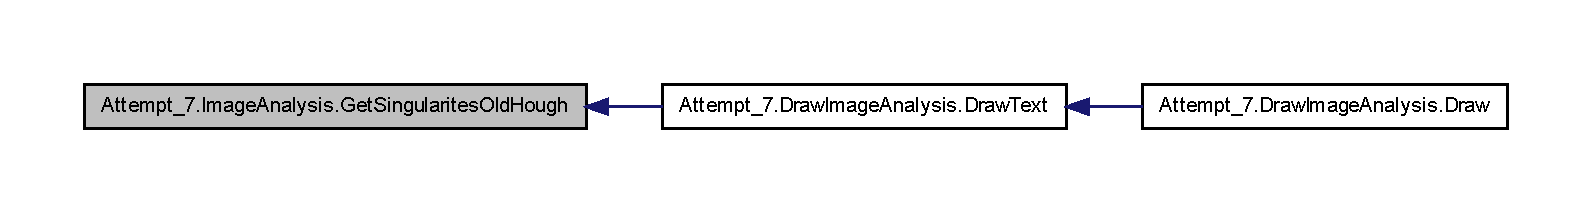
\includegraphics[width=400pt]{class_attempt__7_1_1_image_analysis_a8b8e7e705c97bbb5da1300c139ec0f36_icgraph}
\end{center}
\end{figure}


\index{Attempt\_\-7::ImageAnalysis@{Attempt\_\-7::ImageAnalysis}!GetSingularitiesNewHough@{GetSingularitiesNewHough}}
\index{GetSingularitiesNewHough@{GetSingularitiesNewHough}!Attempt_7::ImageAnalysis@{Attempt\_\-7::ImageAnalysis}}
\subsubsection[{GetSingularitiesNewHough}]{\setlength{\rightskip}{0pt plus 5cm}int Attempt\_\-7.ImageAnalysis.GetSingularitiesNewHough (
\begin{DoxyParamCaption}
{}
\end{DoxyParamCaption}
)}\label{class_attempt__7_1_1_image_analysis_a23adf47c39e8990ae161dd46dcb43846}


Returns the number of times rho=0 in the new hough system. 

\begin{DoxyReturn}{Returns}
number of times rho = 0
\end{DoxyReturn}


Definition at line 360 of file ImageAnalysis2.cs.


\begin{DoxyCode}
        {
            return this.countOfNewHoughSingularities;
        }
\end{DoxyCode}


Here is the caller graph for this function:
\nopagebreak
\begin{figure}[H]
\begin{center}
\leavevmode
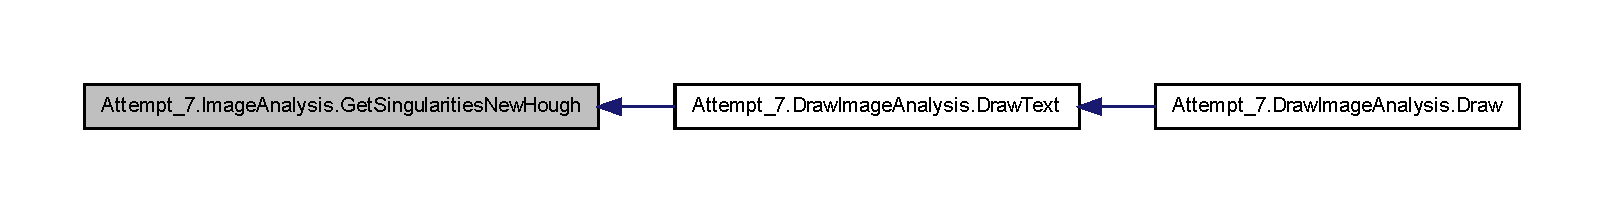
\includegraphics[width=400pt]{class_attempt__7_1_1_image_analysis_a23adf47c39e8990ae161dd46dcb43846_icgraph}
\end{center}
\end{figure}


\index{Attempt\_\-7::ImageAnalysis@{Attempt\_\-7::ImageAnalysis}!GetTrueFalseMaptoDraw@{GetTrueFalseMaptoDraw}}
\index{GetTrueFalseMaptoDraw@{GetTrueFalseMaptoDraw}!Attempt_7::ImageAnalysis@{Attempt\_\-7::ImageAnalysis}}
\subsubsection[{GetTrueFalseMaptoDraw}]{\setlength{\rightskip}{0pt plus 5cm}bool [,] Attempt\_\-7.ImageAnalysis.GetTrueFalseMaptoDraw (
\begin{DoxyParamCaption}
{}
\end{DoxyParamCaption}
)}\label{class_attempt__7_1_1_image_analysis_a1ba8eee3151c73ef5023003ee7b57b67}


Allows access to the bool map that is to be drawn. 

\begin{DoxyReturn}{Returns}
bool map
\end{DoxyReturn}


Definition at line 313 of file ImageAnalysis2.cs.


\begin{DoxyCode}
        {
            return this.trueFalseMapC;
        }
\end{DoxyCode}


Here is the caller graph for this function:\nopagebreak
\begin{figure}[H]
\begin{center}
\leavevmode
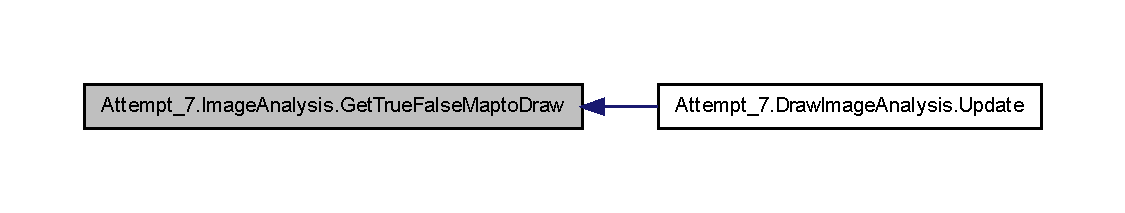
\includegraphics[width=400pt]{class_attempt__7_1_1_image_analysis_a1ba8eee3151c73ef5023003ee7b57b67_icgraph}
\end{center}
\end{figure}


\index{Attempt\_\-7::ImageAnalysis@{Attempt\_\-7::ImageAnalysis}!GetTurnIndicator@{GetTurnIndicator}}
\index{GetTurnIndicator@{GetTurnIndicator}!Attempt_7::ImageAnalysis@{Attempt\_\-7::ImageAnalysis}}
\subsubsection[{GetTurnIndicator}]{\setlength{\rightskip}{0pt plus 5cm}int Attempt\_\-7.ImageAnalysis.GetTurnIndicator (
\begin{DoxyParamCaption}
{}
\end{DoxyParamCaption}
)}\label{class_attempt__7_1_1_image_analysis_a99c5e65fe48a1145d7c9afba96bfb220}


Allows the \doxyref{SimulationMain}{p.}{class_attempt__7_1_1_simulation_main} to get the turnIndicator. 

\begin{DoxyReturn}{Returns}
The turn Indicator
\end{DoxyReturn}


Definition at line 351 of file ImageAnalysis2.cs.


\begin{DoxyCode}
        {
            return this.turnIndication;
        }
\end{DoxyCode}


Here is the caller graph for this function:\nopagebreak
\begin{figure}[H]
\begin{center}
\leavevmode
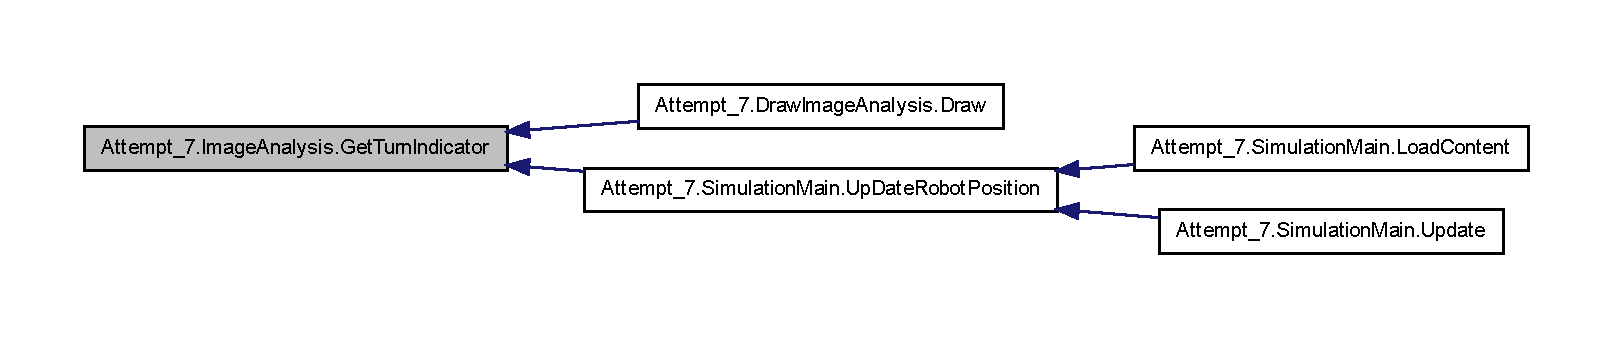
\includegraphics[width=400pt]{class_attempt__7_1_1_image_analysis_a99c5e65fe48a1145d7c9afba96bfb220_icgraph}
\end{center}
\end{figure}


\index{Attempt\_\-7::ImageAnalysis@{Attempt\_\-7::ImageAnalysis}!GetWhiteCount@{GetWhiteCount}}
\index{GetWhiteCount@{GetWhiteCount}!Attempt_7::ImageAnalysis@{Attempt\_\-7::ImageAnalysis}}
\subsubsection[{GetWhiteCount}]{\setlength{\rightskip}{0pt plus 5cm}int Attempt\_\-7.ImageAnalysis.GetWhiteCount (
\begin{DoxyParamCaption}
{}
\end{DoxyParamCaption}
)}\label{class_attempt__7_1_1_image_analysis_a55b77047aaacc5a78fcd70401da3b069}


Allows access to the WhiteCount in the image. 

\begin{DoxyReturn}{Returns}
The number of white pixels
\end{DoxyReturn}


Definition at line 295 of file ImageAnalysis2.cs.


\begin{DoxyCode}
        {
            return this.totalWhiteCnt;
        }
\end{DoxyCode}


Here is the caller graph for this function:\nopagebreak
\begin{figure}[H]
\begin{center}
\leavevmode
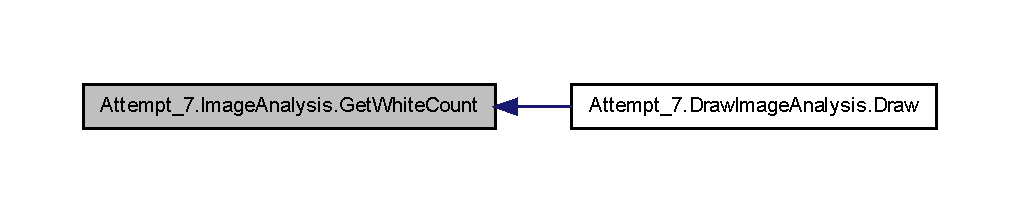
\includegraphics[width=400pt]{class_attempt__7_1_1_image_analysis_a55b77047aaacc5a78fcd70401da3b069_icgraph}
\end{center}
\end{figure}


\index{Attempt\_\-7::ImageAnalysis@{Attempt\_\-7::ImageAnalysis}!Hough@{Hough}}
\index{Hough@{Hough}!Attempt_7::ImageAnalysis@{Attempt\_\-7::ImageAnalysis}}
\subsubsection[{Hough}]{\setlength{\rightskip}{0pt plus 5cm}void Attempt\_\-7.ImageAnalysis.Hough (
\begin{DoxyParamCaption}
\item[{bool}]{isLine[,]}
\end{DoxyParamCaption}
)\hspace{0.3cm}{\ttfamily  [private]}}\label{class_attempt__7_1_1_image_analysis_a89a87d17049aa2c3f1b31af9b8ffcb07}


For each white pixel that might be part of a line, Find all the potiential lines going through it and store each vote for that line in the accumlator's bins. Calls the methods to search through the accumlator to find the bins with the largest values. 


\begin{DoxyParams}{Parameters}
{\em isLine} & The trueFalse array of pixels that might be part of a line. \\
\hline
\end{DoxyParams}


Definition at line 823 of file ImageAnalysis2.cs.


\begin{DoxyCode}
        {
            // Find all possible lines through each point and put into array bin.
      
            for (short x = this.count1E; x < this.screenWidth; x += 
      UpdateSquareDimForAnalysis)
            {
                for (short y = this.count2E; y < this.screenHeight; y += 
      UpdateSquareDimForAnalysis)
                {
                    if (isLine[x, y] == true)
                    {
                        if (this.currentMode == New_HOUGH_MODE)
                        {
                            for (short theta = 0; theta < 180; theta += 
      ThetaIncrement)
                            {
                                // Bottom center = origin. 
                                short xprime = (short)(x - (this.screenWidth / 2)
      );
                                short yprime = (short)(-y + this.screenHeight);
                                short rhoprime = (short)(((xprime * Math.Cos(Math
      Helper.ToRadians(theta))) + (yprime * Math.Sin(MathHelper.ToRadians(theta)))) / 
      RhoIncrement);
                                if (rhoprime >= 0)
                                {
                                    this.accum2[theta / ThetaIncrement, rhoprime]
      ++;
                                }

                                // because that would represent a line that is no
      t on the screen
                                else 
                                {
                                    this.accum2[(theta + 180) / ThetaIncrement, -
      rhoprime]++;
                                }


                            }
                        }

                        if (this.currentMode == OLD_HOUGH_MODE)
                        {
                            for (short theta = -180; theta < 180; theta += 
      ThetaIncrement)
                            {
                                short rho = (short)(((x * Math.Cos(MathHelper.ToR
      adians(theta))) + (y * Math.Sin(MathHelper.ToRadians(theta)))) / RhoIncrement);
                                if (rho > 0)
                                {
                                    this.accum1[(theta + 180) / ThetaIncrement, r
      ho]++;
                                }
                            }
                        }
                    }
                }
            }

            this.count1E++;
            if (this.count1E == UpdateSquareDimForAnalysis)
            {
                this.count1E = 0;
                this.count2E++;
                if (this.count2E == UpdateSquareDimForAnalysis)
                {
                    // Find the largest values. 
                    for (int i = 0; i < NumberofLinesToFind; i++)
                    {
                        if (this.currentMode == New_HOUGH_MODE)
                        {
                            this.FindMaxInAccumArrayOfHough(this.accum2, 
      ThetaIncrement, (short)(i * 11));
                            this.CalculateStartandStopofLine(this.houghInfo[4 + (
      i * 11)], this.houghInfo[5 + (i * 11)], this.houghInfo[0 + (i * 11)], i * 4);
                            this.ClearMaxInAccum(this.accum2, (int)this.
      houghInfo[(i * 11) + 2], (int)this.houghInfo[(i * 11) + 3]);
                        }

                        if (this.currentMode == OLD_HOUGH_MODE)
                        {
                            this.FindMaxInAccumArrayOfHough(this.accum1, 
      ThetaIncrement, (short)(i * 11));
                            this.CalculateStartandStopofLine(this.houghInfo[4 + (
      i * 11)], this.houghInfo[5 + (i * 11)], this.houghInfo[0 + (i * 11)], i * 4);

                            // From top (0,0) to perpendicular
                            this.houghLineStartandStopVectors[i * 4 + 2] = new Ve
      ctor3((float)this.houghInfo[i * 11 + 4], (float)this.houghInfo[i * 11 + 5], 0);

                            // From bottom center to perpendicular
                            this.houghLineStartandStopVectors[i * 4 + 3] = new Ve
      ctor3((float)this.houghInfo[i * 11 + 7], (float)this.houghInfo[i * 11 + 8], 0);

                            this.ClearMaxInAccum(this.accum1, (int)this.
      houghInfo[(i * 11) + 2], (int)this.houghInfo[(i * 11) + 3]);
                        }
                    }

                    if (this.currentMode == New_HOUGH_MODE)
                    {
                        this.FindAverages(); // Find the average rho and theta
                        Array.Clear(this.accum2, 0, this.accum2.Length); // Clear
       the accumulator
                    }

                    if (this.currentMode == OLD_HOUGH_MODE)
                    {
                        Array.Clear(this.accum1, 0, this.accum1.Length); // Clear
       the accumulator                       

                    }

                    this.count2E = 0;
                }
            }
        }
\end{DoxyCode}


Here is the call graph for this function:
\nopagebreak
\begin{figure}[H]
\begin{center}
\leavevmode
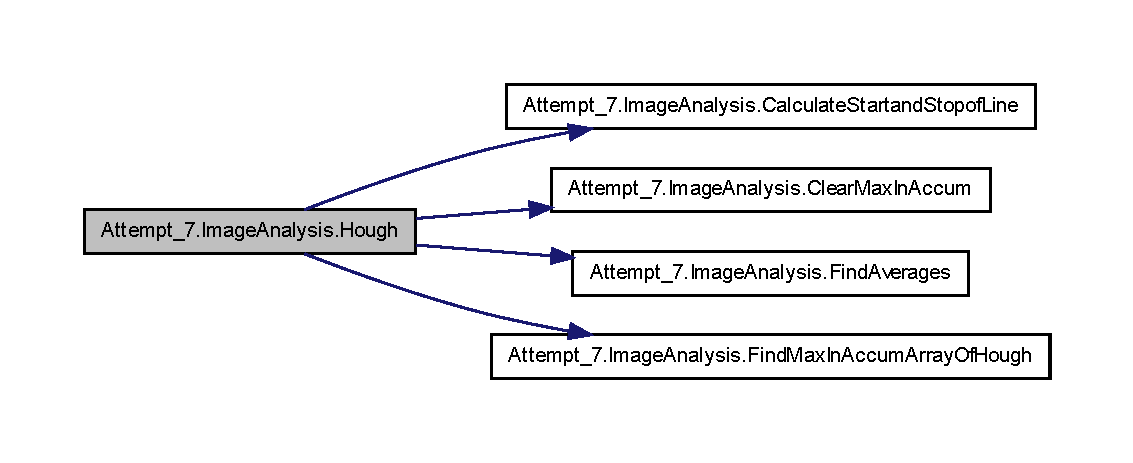
\includegraphics[width=400pt]{class_attempt__7_1_1_image_analysis_a89a87d17049aa2c3f1b31af9b8ffcb07_cgraph}
\end{center}
\end{figure}




Here is the caller graph for this function:\nopagebreak
\begin{figure}[H]
\begin{center}
\leavevmode
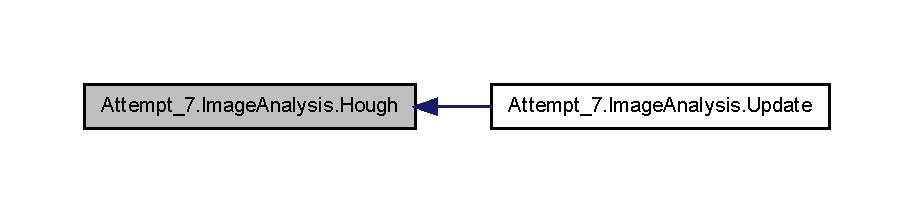
\includegraphics[width=400pt]{class_attempt__7_1_1_image_analysis_a89a87d17049aa2c3f1b31af9b8ffcb07_icgraph}
\end{center}
\end{figure}


\index{Attempt\_\-7::ImageAnalysis@{Attempt\_\-7::ImageAnalysis}!Initialize@{Initialize}}
\index{Initialize@{Initialize}!Attempt_7::ImageAnalysis@{Attempt\_\-7::ImageAnalysis}}
\subsubsection[{Initialize}]{\setlength{\rightskip}{0pt plus 5cm}override void Attempt\_\-7.ImageAnalysis.Initialize (
\begin{DoxyParamCaption}
{}
\end{DoxyParamCaption}
)}\label{class_attempt__7_1_1_image_analysis_af250995c0e8937dc0ad3c26239716225}


Called when the class is initialized. Creates many of the arrays and sets many of the values. 



Definition at line 218 of file ImageAnalysis2.cs.


\begin{DoxyCode}
        {
            // Create the arrays needed. Building them now will save CPU later. 
            this.trueFalseMap = new bool[this.screenWidth, this.screenHeight];
            this.trueFalseMapB = new bool[this.screenWidth, this.screenHeight];
            this.trueFalseMapC = new bool[this.screenWidth, this.screenHeight];

            this.accum2 = new short[360 / ThetaIncrement, AccumLength / 
      RhoIncrement]; // Build the accumlator array. Make is smaller or shorter based on
       the size of the rho and theta increments
            this.accum1 = new short[360 / ThetaIncrement, AccumLengthOld / 
      RhoIncrement];
            this.colorArray1D = new Color[this.screenWidth * this.screenHeight]; 
      // Create a 1D array of color
            this.colorArray = new Color[this.screenWidth, this.screenHeight]; // 
      Create a 2D array of color

            this.houghInfo = new double[(11 * NumberofLinesToFind) + 5]; // Make 
      the array to store hough information. Must be double so that slopes which are fra
      ctions can be stored

            // Set the color thresholds
            this.redGood = this.whiteParam;
            this.blueGood = this.whiteParam;
            this.greenGood = this.whiteParam;

            this.houghLineStartandStopVectors = new Vector3[NumberofLinesToFind *
       4];
            for (int i = 0; i < NumberofLinesToFind * 4; i++)
            {
                this.houghLineStartandStopVectors[i] = Vector3.Zero;
            }

            this.middleValues = new int[this.screenHeight]; // Steering desisions
       are based off the average middle clear value for each row

            base.Initialize();
        }
\end{DoxyCode}
\index{Attempt\_\-7::ImageAnalysis@{Attempt\_\-7::ImageAnalysis}!SetRobotCameraView@{SetRobotCameraView}}
\index{SetRobotCameraView@{SetRobotCameraView}!Attempt_7::ImageAnalysis@{Attempt\_\-7::ImageAnalysis}}
\subsubsection[{SetRobotCameraView}]{\setlength{\rightskip}{0pt plus 5cm}void Attempt\_\-7.ImageAnalysis.SetRobotCameraView (
\begin{DoxyParamCaption}
\item[{Texture2D}]{text}
\end{DoxyParamCaption}
)}\label{class_attempt__7_1_1_image_analysis_aa6cac5de12d6bf454500ee5498db48cb}


Takes a 2D renderTarget/Texture and sets it as the image to analze. Explicitly called in the \doxyref{SimulationMain}{p.}{class_attempt__7_1_1_simulation_main} Draw Method. 


\begin{DoxyParams}{Parameters}
{\em text} & The texture to analze. \\
\hline
\end{DoxyParams}


Definition at line 264 of file ImageAnalysis2.cs.


\begin{DoxyCode}
        {
            this.robotCameraView = text;
        }
\end{DoxyCode}


Here is the caller graph for this function:\nopagebreak
\begin{figure}[H]
\begin{center}
\leavevmode
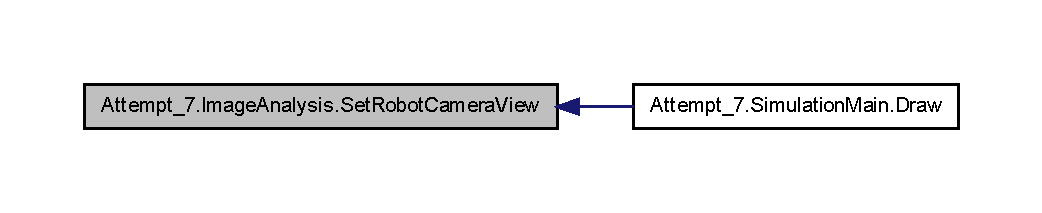
\includegraphics[width=400pt]{class_attempt__7_1_1_image_analysis_aa6cac5de12d6bf454500ee5498db48cb_icgraph}
\end{center}
\end{figure}


\index{Attempt\_\-7::ImageAnalysis@{Attempt\_\-7::ImageAnalysis}!ShowPath@{ShowPath}}
\index{ShowPath@{ShowPath}!Attempt_7::ImageAnalysis@{Attempt\_\-7::ImageAnalysis}}
\subsubsection[{ShowPath}]{\setlength{\rightskip}{0pt plus 5cm}bool [,] Attempt\_\-7.ImageAnalysis.ShowPath (
\begin{DoxyParamCaption}
\item[{bool}]{blocked[,], }
\item[{bool}]{clearPath[,]}
\end{DoxyParamCaption}
)\hspace{0.3cm}{\ttfamily  [private]}}\label{class_attempt__7_1_1_image_analysis_a0befd0244fb507716329010283730fb6}


Find a path through the map to go through and return it as a bool map, also set the turn indicator. Based off the reactiveNavigation from the old robot code. 


\begin{DoxyParams}{Parameters}
{\em blocked} & The trueFalse map of pixels that are blocked.\\
\hline
{\em clearPath} & Blank. This map will be turned.\\
\hline
\end{DoxyParams}
\begin{DoxyReturn}{Returns}
The trueFalse map of a clear path.
\end{DoxyReturn}


Definition at line 550 of file ImageAnalysis2.cs.


\begin{DoxyCode}
        {
            int lastRightX = this.screenWidth, lastLeftX = 0;
            int leftX, rightX;
            int sum = 0;

            for (int rowNumber = this.screenHeight - this.count1D - 1; rowNumber 
      > 0; rowNumber -= UpdateSquareDimForAnalysis)
            {
                // Start in the middle
                leftX = (int)((lastLeftX + lastRightX) / 2);

                // Search starting in the middle and bottom of picture and go lef
      t (i.e. subtract) for a blocked pixel
                while (leftX > lastLeftX && blocked[leftX, rowNumber] == false)
                {
                    clearPath[leftX, rowNumber] = true;
                    leftX--;
                }

                // Start in the middle and bottome go right 
                rightX = (int)((lastLeftX + lastRightX) / 2);

                while (rightX < lastRightX && blocked[rightX, rowNumber] == false
      )
                {
                    clearPath[rightX, rowNumber] = true;
                    rightX++;
                }

                lastLeftX = leftX;
                lastRightX = rightX;
                sum += (int)((lastLeftX + lastRightX) / 2);
            }

            this.count1D++;
            if (this.count1D == UpdateSquareDimForAnalysis)
            {
                this.count1D = 0;
            }

            // Find the average middle pixels for each row and set the turn indic
      ator based on this value. 
            this.turnIndication = ((sum * UpdateSquareDimForAnalysis) / this.
      screenHeight) - (this.screenWidth / 2);
            return clearPath;
        }
\end{DoxyCode}


Here is the caller graph for this function:\nopagebreak
\begin{figure}[H]
\begin{center}
\leavevmode
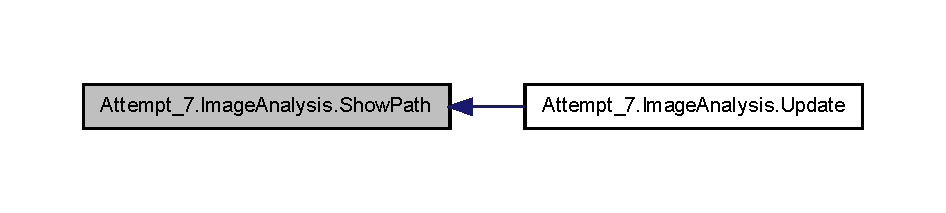
\includegraphics[width=400pt]{class_attempt__7_1_1_image_analysis_a0befd0244fb507716329010283730fb6_icgraph}
\end{center}
\end{figure}


\index{Attempt\_\-7::ImageAnalysis@{Attempt\_\-7::ImageAnalysis}!Smooth@{Smooth}}
\index{Smooth@{Smooth}!Attempt_7::ImageAnalysis@{Attempt\_\-7::ImageAnalysis}}
\subsubsection[{Smooth}]{\setlength{\rightskip}{0pt plus 5cm}bool [,] Attempt\_\-7.ImageAnalysis.Smooth (
\begin{DoxyParamCaption}
\item[{bool}]{original[,], }
\item[{bool}]{final[,]}
\end{DoxyParamCaption}
)\hspace{0.3cm}{\ttfamily  [private]}}\label{class_attempt__7_1_1_image_analysis_a87fb97262f08f3b21afd2bcdb29bbe6c}


Takes a truefalse map and for each pixel checks the other pixels around it to see if they are also white. If the number of pixels arround it that are also white is above a threshold then keep that pixel white. Meant to reduce noise in the picture. NOT IN USE RIGHT NOW$\ast$$\ast$$\ast$$\ast$$\ast$$\ast$$\ast$$\ast$$\ast$$\ast$$\ast$$\ast$$\ast$$\ast$$\ast$$\ast$$\ast$$\ast$$\ast$$\ast$. 


\begin{DoxyParams}{Parameters}
{\em original} & The raw truefalse map of whie pixels.\\
\hline
{\em final} & The trueFalse map to modify\\
\hline
\end{DoxyParams}
\begin{DoxyReturn}{Returns}
The truefalse map of pixels that met the threshold requirements. 
\end{DoxyReturn}


Definition at line 489 of file ImageAnalysis2.cs.


\begin{DoxyCode}
        {
            int cnt;
            for (int i = this.count1B; i < this.screenWidth; i += 
      UpdateSquareDimForAnalysis)
            {
                for (int j = this.count2B; j < this.screenHeight; j += 
      UpdateSquareDimForAnalysis)
                {
                    if (original[i, j] == true)
                    {
                        cnt = 0;
                        for (int a = -SmoothSearchSize; a <= SmoothSearchSize; a+
      +)
                        {
                            for (int b = -SmoothSearchSize; b <= 
      SmoothSearchSize; b++)
                            {
                                if (i + a > -1 && i + a < this.screenWidth && j +
       b > -1 && j + b < this.screenHeight)
                                {
                                    if (original[i + a, j + b] == true)
                                    {
                                        cnt = cnt + 1;
                                    }
                                }
                            }
                        }

                        if (cnt > this.cntThreshold)
                        {
                            final[i, j] = true;
                        }
                        else
                        {
                            final[i, j] = false;
                        }
                    }
                    else
                    {
                        final[i, j] = false;
                    }
                }
            }

            this.count1B++;
            if (this.count1B == UpdateSquareDimForDrawing)
            {
                this.count1B = 0;
                this.count2B++;
                if (this.count2B == UpdateSquareDimForDrawing)
                {
                    this.count2B = 0;
                }
            }

            return final;
        }
\end{DoxyCode}
\index{Attempt\_\-7::ImageAnalysis@{Attempt\_\-7::ImageAnalysis}!TextureTo2DArray@{TextureTo2DArray}}
\index{TextureTo2DArray@{TextureTo2DArray}!Attempt_7::ImageAnalysis@{Attempt\_\-7::ImageAnalysis}}
\subsubsection[{TextureTo2DArray}]{\setlength{\rightskip}{0pt plus 5cm}Color [,] Attempt\_\-7.ImageAnalysis.TextureTo2DArray (
\begin{DoxyParamCaption}
\item[{Texture2D}]{texture, }
\item[{Color[$\,$]}]{colors1D, }
\item[{Color}]{colors2D[,]}
\end{DoxyParamCaption}
)\hspace{0.3cm}{\ttfamily  [private]}}\label{class_attempt__7_1_1_image_analysis_ac70a680405b76bd8b0ece8ee2a8112e8}


Takes a texture and makes it into a 2D color array. Passing in the arrays is faster than trying to build it each time. 


\begin{DoxyParams}{Parameters}
{\em texture} & Texture to extract color information\\
\hline
{\em colors1D} & 1D array needed for the extraction\\
\hline
{\em colors2D} & 2D array that will be returned\\
\hline
\end{DoxyParams}
\begin{DoxyReturn}{Returns}
The 2D color array of the texture color information
\end{DoxyReturn}


Definition at line 390 of file ImageAnalysis2.cs.


\begin{DoxyCode}
        {
            texture.GetData(colors1D);
            for (int x = 0; x < texture.Width; x++)
            {
                for (int y = 0; y < texture.Height; y++)
                {
                    colors2D[x, y] = colors1D[x + (y * texture.Width)];
                }
            }

            return colors2D;
        }
\end{DoxyCode}


Here is the caller graph for this function:\nopagebreak
\begin{figure}[H]
\begin{center}
\leavevmode
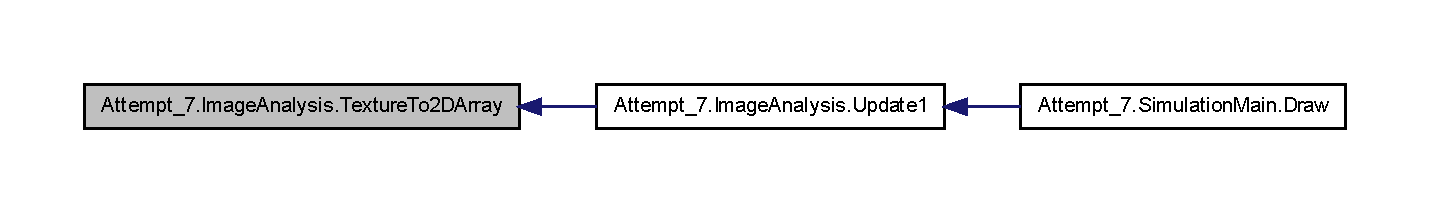
\includegraphics[width=400pt]{class_attempt__7_1_1_image_analysis_ac70a680405b76bd8b0ece8ee2a8112e8_icgraph}
\end{center}
\end{figure}


\index{Attempt\_\-7::ImageAnalysis@{Attempt\_\-7::ImageAnalysis}!Update@{Update}}
\index{Update@{Update}!Attempt_7::ImageAnalysis@{Attempt\_\-7::ImageAnalysis}}
\subsubsection[{Update}]{\setlength{\rightskip}{0pt plus 5cm}override void Attempt\_\-7.ImageAnalysis.Update (
\begin{DoxyParamCaption}
\item[{GameTime}]{gameTime}
\end{DoxyParamCaption}
)}\label{class_attempt__7_1_1_image_analysis_ab597ab75ce16d1fd903b68e7df2a2c7f}


Calls the analysis methods that actually do all the work. Basically the Main function for the Image Analysis Class. 


\begin{DoxyParams}{Parameters}
{\em gameTime} & Clock Info\\
\hline
\end{DoxyParams}


Definition at line 273 of file ImageAnalysis2.cs.


\begin{DoxyCode}
        {
            currentMode = Attempt_7.SimulationMain.currentHoughMode; //Comment ou
      t for the UnitTest only

            if (this.colorArray != null)
            {
                this.trueFalseMapC = this.FindWhite(this.colorArray); // Find Whi
      te                
                this.Hough(this.trueFalseMapC); // Run the hough  
                if (this.turnIndicatorisTheta != true)
                {
                    this.trueFalseMap = this.ShowPath(this.trueFalseMapC, this.
      trueFalseMapB); // Find the path through the map   
                }

            }
            base.Update(gameTime);
        }
\end{DoxyCode}


Here is the call graph for this function:
\nopagebreak
\begin{figure}[H]
\begin{center}
\leavevmode
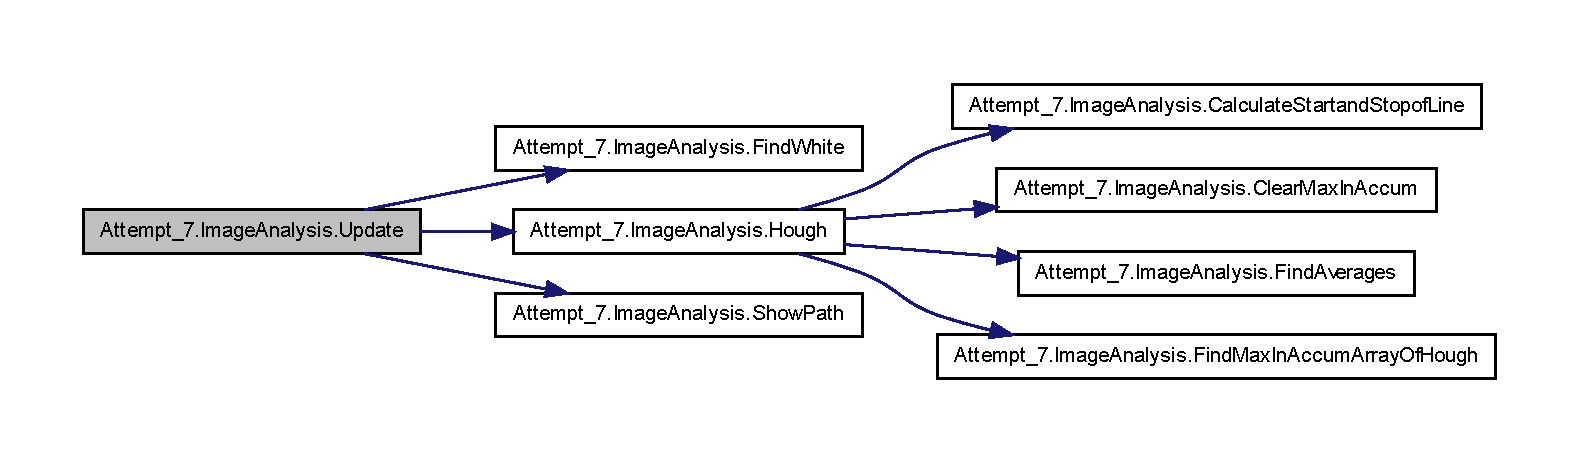
\includegraphics[width=400pt]{class_attempt__7_1_1_image_analysis_ab597ab75ce16d1fd903b68e7df2a2c7f_cgraph}
\end{center}
\end{figure}


\index{Attempt\_\-7::ImageAnalysis@{Attempt\_\-7::ImageAnalysis}!Update1@{Update1}}
\index{Update1@{Update1}!Attempt_7::ImageAnalysis@{Attempt\_\-7::ImageAnalysis}}
\subsubsection[{Update1}]{\setlength{\rightskip}{0pt plus 5cm}void Attempt\_\-7.ImageAnalysis.Update1 (
\begin{DoxyParamCaption}
\item[{GameTime}]{gameTime1}
\end{DoxyParamCaption}
)}\label{class_attempt__7_1_1_image_analysis_a1d0bc75993df71df5d005ab3d749bb81}


Stores the texture from the robot camera in a color array before the texture is disposed. Expicitly called in the \doxyref{SimulationMain}{p.}{class_attempt__7_1_1_simulation_main} Draw method. 


\begin{DoxyParams}{Parameters}
{\em gameTime1} & Clock Information\\
\hline
\end{DoxyParams}


Definition at line 252 of file ImageAnalysis2.cs.


\begin{DoxyCode}
        {
            if (this.robotCameraView != null)
            {
                this.colorArray = this.TextureTo2DArray(this.robotCameraView, thi
      s.colorArray1D, this.colorArray);
            }
        }
\end{DoxyCode}


Here is the call graph for this function:\nopagebreak
\begin{figure}[H]
\begin{center}
\leavevmode
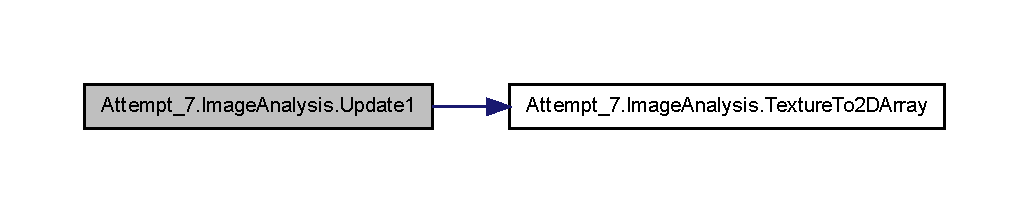
\includegraphics[width=400pt]{class_attempt__7_1_1_image_analysis_a1d0bc75993df71df5d005ab3d749bb81_cgraph}
\end{center}
\end{figure}




Here is the caller graph for this function:\nopagebreak
\begin{figure}[H]
\begin{center}
\leavevmode
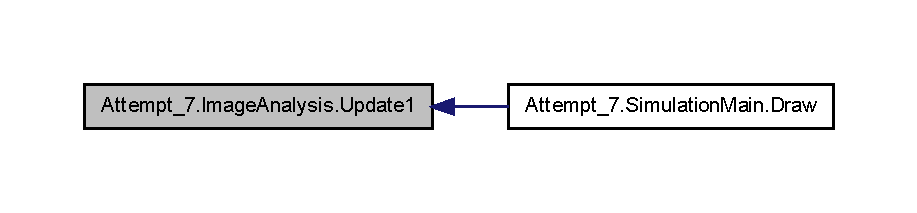
\includegraphics[width=400pt]{class_attempt__7_1_1_image_analysis_a1d0bc75993df71df5d005ab3d749bb81_icgraph}
\end{center}
\end{figure}


\index{Attempt\_\-7::ImageAnalysis@{Attempt\_\-7::ImageAnalysis}!Whiteline@{Whiteline}}
\index{Whiteline@{Whiteline}!Attempt_7::ImageAnalysis@{Attempt\_\-7::ImageAnalysis}}
\subsubsection[{Whiteline}]{\setlength{\rightskip}{0pt plus 5cm}bool [,] Attempt\_\-7.ImageAnalysis.Whiteline (
\begin{DoxyParamCaption}
\item[{bool}]{whitemap[,]}
\end{DoxyParamCaption}
)\hspace{0.3cm}{\ttfamily  [private]}}\label{class_attempt__7_1_1_image_analysis_a879442dce1e8ad7240a78101c31cace4}


Determines if white pixels meet the Width threshold to possibly be a line. NOT IN USE RIGHT NOW$\ast$$\ast$$\ast$$\ast$$\ast$$\ast$$\ast$$\ast$$\ast$$\ast$$\ast$$\ast$$\ast$$\ast$$\ast$$\ast$$\ast$$\ast$$\ast$$\ast$. 


\begin{DoxyParams}{Parameters}
{\em whitemap} & The TrueFalse map of whate Pixels\\
\hline
\end{DoxyParams}
\begin{DoxyReturn}{Returns}
A truefalse map of white pixels that met the line width requirement
\end{DoxyReturn}


Definition at line 444 of file ImageAnalysis2.cs.


\begin{DoxyCode}
        {
            int i, j, b, cnt;
            bool[,] isLine = new bool[(int)this.screenWidth, (int)this.
      screenHeight]; // Make a new array
            for (i = 0; i < this.screenWidth; ++i)
            {
                for (j = 0; j < this.screenHeight; ++j)
                {
                    if (whitemap[i, j] == true)
                    {
                        cnt = 0;
                        for (b = 0; b <= 25; b++)
                        {
                            if (j + b < this.screenHeight && whitemap[i, j + b] =
      = true)
                            {
                                cnt = cnt + 1;
                            }
                        }

                        if (cnt > 3 && cnt < 15)
                        {
                            isLine[i, j] = true;
                        }
                        else
                        {
                            isLine[i, j] = false;
                        }
                    }
                    else
                    {
                        isLine[i, j] = false;
                    }
                }
            }

            return isLine;
        }
\end{DoxyCode}


\subsection{Member Data Documentation}
\index{Attempt\_\-7::ImageAnalysis@{Attempt\_\-7::ImageAnalysis}!accum1@{accum1}}
\index{accum1@{accum1}!Attempt_7::ImageAnalysis@{Attempt\_\-7::ImageAnalysis}}
\subsubsection[{accum1}]{\setlength{\rightskip}{0pt plus 5cm}short [,] {\bf Attempt\_\-7.ImageAnalysis.accum1}\hspace{0.3cm}{\ttfamily  [private]}}\label{class_attempt__7_1_1_image_analysis_acb2ae3d661927b0467b5d4fdc7eded98}


Definition at line 172 of file ImageAnalysis2.cs.

\index{Attempt\_\-7::ImageAnalysis@{Attempt\_\-7::ImageAnalysis}!accum2@{accum2}}
\index{accum2@{accum2}!Attempt_7::ImageAnalysis@{Attempt\_\-7::ImageAnalysis}}
\subsubsection[{accum2}]{\setlength{\rightskip}{0pt plus 5cm}short [,] {\bf Attempt\_\-7.ImageAnalysis.accum2}\hspace{0.3cm}{\ttfamily  [private]}}\label{class_attempt__7_1_1_image_analysis_ac861772cdcfacb7ac2401079c651eb4e}


The accumlator for the hough values. Each position is a hough Bin. Each bin represents a line in Cartessian cordinates. The Accumlator is basically in polar cordinates. Theta,rho. 



Definition at line 171 of file ImageAnalysis2.cs.

\index{Attempt\_\-7::ImageAnalysis@{Attempt\_\-7::ImageAnalysis}!AccumLength@{AccumLength}}
\index{AccumLength@{AccumLength}!Attempt_7::ImageAnalysis@{Attempt\_\-7::ImageAnalysis}}
\subsubsection[{AccumLength}]{\setlength{\rightskip}{0pt plus 5cm}const int {\bf Attempt\_\-7.ImageAnalysis.AccumLength} = 600\hspace{0.3cm}{\ttfamily  [private]}}\label{class_attempt__7_1_1_image_analysis_a8cdd9f3be232a5cf32006ddd52bc4ae2}


Size of the Acuumlator's lenght. Must be able to fit the largest posible value of rho. Max rho = Sqrt( ScreenHeight$^\wedge$2+ (ScreenWidth/2)$^\wedge$2), because the origin is the bottom center and the max rho is top left or right. 



Definition at line 46 of file ImageAnalysis2.cs.

\index{Attempt\_\-7::ImageAnalysis@{Attempt\_\-7::ImageAnalysis}!AccumLengthOld@{AccumLengthOld}}
\index{AccumLengthOld@{AccumLengthOld}!Attempt_7::ImageAnalysis@{Attempt\_\-7::ImageAnalysis}}
\subsubsection[{AccumLengthOld}]{\setlength{\rightskip}{0pt plus 5cm}const int {\bf Attempt\_\-7.ImageAnalysis.AccumLengthOld} = 810\hspace{0.3cm}{\ttfamily  [private]}}\label{class_attempt__7_1_1_image_analysis_a75787da0f52a71c54f5f8a18d32467b8}


lenght of the hold hough accumulator 



Definition at line 51 of file ImageAnalysis2.cs.

\index{Attempt\_\-7::ImageAnalysis@{Attempt\_\-7::ImageAnalysis}!blueGood@{blueGood}}
\index{blueGood@{blueGood}!Attempt_7::ImageAnalysis@{Attempt\_\-7::ImageAnalysis}}
\subsubsection[{blueGood}]{\setlength{\rightskip}{0pt plus 5cm}int {\bf Attempt\_\-7.ImageAnalysis.blueGood}\hspace{0.3cm}{\ttfamily  [private]}}\label{class_attempt__7_1_1_image_analysis_afdb8b1b0ef151cceeed6883a6ca955f5}


Definition at line 182 of file ImageAnalysis2.cs.

\index{Attempt\_\-7::ImageAnalysis@{Attempt\_\-7::ImageAnalysis}!ClearArroundMaxDegree@{ClearArroundMaxDegree}}
\index{ClearArroundMaxDegree@{ClearArroundMaxDegree}!Attempt_7::ImageAnalysis@{Attempt\_\-7::ImageAnalysis}}
\subsubsection[{ClearArroundMaxDegree}]{\setlength{\rightskip}{0pt plus 5cm}const int {\bf Attempt\_\-7.ImageAnalysis.ClearArroundMaxDegree} = 5\hspace{0.3cm}{\ttfamily  [private]}}\label{class_attempt__7_1_1_image_analysis_af57eb11bc470f90921bed1b60cfc9741}


Number of degrees around a maximum to clear around before searching the Accumulator again. 



Definition at line 76 of file ImageAnalysis2.cs.

\index{Attempt\_\-7::ImageAnalysis@{Attempt\_\-7::ImageAnalysis}!ClearArroundMaxRho@{ClearArroundMaxRho}}
\index{ClearArroundMaxRho@{ClearArroundMaxRho}!Attempt_7::ImageAnalysis@{Attempt\_\-7::ImageAnalysis}}
\subsubsection[{ClearArroundMaxRho}]{\setlength{\rightskip}{0pt plus 5cm}const int {\bf Attempt\_\-7.ImageAnalysis.ClearArroundMaxRho} = 8\hspace{0.3cm}{\ttfamily  [private]}}\label{class_attempt__7_1_1_image_analysis_a5de31952bf3d80b7ad21aa4c0acc3092}


Number of rho values around a maximum to clear around before searching the Accumulator again. 



Definition at line 81 of file ImageAnalysis2.cs.

\index{Attempt\_\-7::ImageAnalysis@{Attempt\_\-7::ImageAnalysis}!cntThreshold@{cntThreshold}}
\index{cntThreshold@{cntThreshold}!Attempt_7::ImageAnalysis@{Attempt\_\-7::ImageAnalysis}}
\subsubsection[{cntThreshold}]{\setlength{\rightskip}{0pt plus 5cm}int {\bf Attempt\_\-7.ImageAnalysis.cntThreshold} = 15\hspace{0.3cm}{\ttfamily  [private]}}\label{class_attempt__7_1_1_image_analysis_ae51a397ecb99b137ec6920e1329e8b6b}


Used by the smooth method. How many pixels must also be white in the area around a white pixel for it to be counted white. 



Definition at line 177 of file ImageAnalysis2.cs.

\index{Attempt\_\-7::ImageAnalysis@{Attempt\_\-7::ImageAnalysis}!colorArray@{colorArray}}
\index{colorArray@{colorArray}!Attempt_7::ImageAnalysis@{Attempt\_\-7::ImageAnalysis}}
\subsubsection[{colorArray}]{\setlength{\rightskip}{0pt plus 5cm}Color [,] {\bf Attempt\_\-7.ImageAnalysis.colorArray}\hspace{0.3cm}{\ttfamily  [private]}}\label{class_attempt__7_1_1_image_analysis_a3490343b5c67fcbbdbb23257a56e4b3a}


Color Array 2D from the robot camera that is analzed. 



Definition at line 141 of file ImageAnalysis2.cs.

\index{Attempt\_\-7::ImageAnalysis@{Attempt\_\-7::ImageAnalysis}!colorArray1D@{colorArray1D}}
\index{colorArray1D@{colorArray1D}!Attempt_7::ImageAnalysis@{Attempt\_\-7::ImageAnalysis}}
\subsubsection[{colorArray1D}]{\setlength{\rightskip}{0pt plus 5cm}Color [$\,$] {\bf Attempt\_\-7.ImageAnalysis.colorArray1D}\hspace{0.3cm}{\ttfamily  [private]}}\label{class_attempt__7_1_1_image_analysis_acdb050a1334538156f7a3332ae7f332a}


Color Array 2D from the robot camera that is analzed. Can't extract informatino directly from the robot view Texture to 2D. But have to go through 1D array. 



Definition at line 146 of file ImageAnalysis2.cs.

\index{Attempt\_\-7::ImageAnalysis@{Attempt\_\-7::ImageAnalysis}!count1A@{count1A}}
\index{count1A@{count1A}!Attempt_7::ImageAnalysis@{Attempt\_\-7::ImageAnalysis}}
\subsubsection[{count1A}]{\setlength{\rightskip}{0pt plus 5cm}short {\bf Attempt\_\-7.ImageAnalysis.count1A} = 0\hspace{0.3cm}{\ttfamily  [private]}}\label{class_attempt__7_1_1_image_analysis_a8fa0aaf56dde7fca58135cdc8c74575f}


These values are the incremented numbers used in the giant double \char`\"{}for-\/loops\char`\"{}. The \char`\"{}1\char`\"{} values are the for the first \char`\"{}for-\/loop\char`\"{}. 



Definition at line 151 of file ImageAnalysis2.cs.

\index{Attempt\_\-7::ImageAnalysis@{Attempt\_\-7::ImageAnalysis}!count1B@{count1B}}
\index{count1B@{count1B}!Attempt_7::ImageAnalysis@{Attempt\_\-7::ImageAnalysis}}
\subsubsection[{count1B}]{\setlength{\rightskip}{0pt plus 5cm}short {\bf Attempt\_\-7.ImageAnalysis.count1B} = 1\hspace{0.3cm}{\ttfamily  [private]}}\label{class_attempt__7_1_1_image_analysis_a53eb6ffb4fdd39ce7f8f59a7358e2144}


Definition at line 151 of file ImageAnalysis2.cs.

\index{Attempt\_\-7::ImageAnalysis@{Attempt\_\-7::ImageAnalysis}!count1C@{count1C}}
\index{count1C@{count1C}!Attempt_7::ImageAnalysis@{Attempt\_\-7::ImageAnalysis}}
\subsubsection[{count1C}]{\setlength{\rightskip}{0pt plus 5cm}short {\bf Attempt\_\-7.ImageAnalysis.count1C} = 0\hspace{0.3cm}{\ttfamily  [private]}}\label{class_attempt__7_1_1_image_analysis_a87af8ae466e41feca21cb200e3463bf9}


Definition at line 151 of file ImageAnalysis2.cs.

\index{Attempt\_\-7::ImageAnalysis@{Attempt\_\-7::ImageAnalysis}!count1D@{count1D}}
\index{count1D@{count1D}!Attempt_7::ImageAnalysis@{Attempt\_\-7::ImageAnalysis}}
\subsubsection[{count1D}]{\setlength{\rightskip}{0pt plus 5cm}short {\bf Attempt\_\-7.ImageAnalysis.count1D} = 1\hspace{0.3cm}{\ttfamily  [private]}}\label{class_attempt__7_1_1_image_analysis_a195927d24332255e0130b0bf2791e146}


Definition at line 151 of file ImageAnalysis2.cs.

\index{Attempt\_\-7::ImageAnalysis@{Attempt\_\-7::ImageAnalysis}!count1E@{count1E}}
\index{count1E@{count1E}!Attempt_7::ImageAnalysis@{Attempt\_\-7::ImageAnalysis}}
\subsubsection[{count1E}]{\setlength{\rightskip}{0pt plus 5cm}short {\bf Attempt\_\-7.ImageAnalysis.count1E} = 0\hspace{0.3cm}{\ttfamily  [private]}}\label{class_attempt__7_1_1_image_analysis_aea1d803966f442e9699b52e196613f8c}


Definition at line 151 of file ImageAnalysis2.cs.

\index{Attempt\_\-7::ImageAnalysis@{Attempt\_\-7::ImageAnalysis}!count2A@{count2A}}
\index{count2A@{count2A}!Attempt_7::ImageAnalysis@{Attempt\_\-7::ImageAnalysis}}
\subsubsection[{count2A}]{\setlength{\rightskip}{0pt plus 5cm}short {\bf Attempt\_\-7.ImageAnalysis.count2A} = 0\hspace{0.3cm}{\ttfamily  [private]}}\label{class_attempt__7_1_1_image_analysis_ae79ba8e9b9e910edf5aded0604399f07}


These values are the incremented numbers used in the giant double \char`\"{}for-\/loops\char`\"{}. The \char`\"{}2\char`\"{} values are the for the second \char`\"{}for-\/loop\char`\"{}. 



Definition at line 156 of file ImageAnalysis2.cs.

\index{Attempt\_\-7::ImageAnalysis@{Attempt\_\-7::ImageAnalysis}!count2B@{count2B}}
\index{count2B@{count2B}!Attempt_7::ImageAnalysis@{Attempt\_\-7::ImageAnalysis}}
\subsubsection[{count2B}]{\setlength{\rightskip}{0pt plus 5cm}short {\bf Attempt\_\-7.ImageAnalysis.count2B} = 0\hspace{0.3cm}{\ttfamily  [private]}}\label{class_attempt__7_1_1_image_analysis_aa9956634aa2f4b718beb2d398b3d2b46}


Definition at line 156 of file ImageAnalysis2.cs.

\index{Attempt\_\-7::ImageAnalysis@{Attempt\_\-7::ImageAnalysis}!count2C@{count2C}}
\index{count2C@{count2C}!Attempt_7::ImageAnalysis@{Attempt\_\-7::ImageAnalysis}}
\subsubsection[{count2C}]{\setlength{\rightskip}{0pt plus 5cm}short {\bf Attempt\_\-7.ImageAnalysis.count2C} = 0\hspace{0.3cm}{\ttfamily  [private]}}\label{class_attempt__7_1_1_image_analysis_a8f2510e6449b532e0a8aa7c616d8f474}


Definition at line 156 of file ImageAnalysis2.cs.

\index{Attempt\_\-7::ImageAnalysis@{Attempt\_\-7::ImageAnalysis}!count2E@{count2E}}
\index{count2E@{count2E}!Attempt_7::ImageAnalysis@{Attempt\_\-7::ImageAnalysis}}
\subsubsection[{count2E}]{\setlength{\rightskip}{0pt plus 5cm}short {\bf Attempt\_\-7.ImageAnalysis.count2E} = 0\hspace{0.3cm}{\ttfamily  [private]}}\label{class_attempt__7_1_1_image_analysis_a1c9acb58142af8f283eb7958305b4337}


Definition at line 156 of file ImageAnalysis2.cs.

\index{Attempt\_\-7::ImageAnalysis@{Attempt\_\-7::ImageAnalysis}!countOfNewHoughSingularities@{countOfNewHoughSingularities}}
\index{countOfNewHoughSingularities@{countOfNewHoughSingularities}!Attempt_7::ImageAnalysis@{Attempt\_\-7::ImageAnalysis}}
\subsubsection[{countOfNewHoughSingularities}]{\setlength{\rightskip}{0pt plus 5cm}int {\bf Attempt\_\-7.ImageAnalysis.countOfNewHoughSingularities} = 0\hspace{0.3cm}{\ttfamily  [private]}}\label{class_attempt__7_1_1_image_analysis_af6c217c696c6b6e16d8988e89d39666b}


Definition at line 194 of file ImageAnalysis2.cs.

\index{Attempt\_\-7::ImageAnalysis@{Attempt\_\-7::ImageAnalysis}!countofOldHoughSingularities@{countofOldHoughSingularities}}
\index{countofOldHoughSingularities@{countofOldHoughSingularities}!Attempt_7::ImageAnalysis@{Attempt\_\-7::ImageAnalysis}}
\subsubsection[{countofOldHoughSingularities}]{\setlength{\rightskip}{0pt plus 5cm}int {\bf Attempt\_\-7.ImageAnalysis.countofOldHoughSingularities} = 0\hspace{0.3cm}{\ttfamily  [private]}}\label{class_attempt__7_1_1_image_analysis_ab9f59ec453ba211ebc7cd614c6ab5fab}


Definition at line 195 of file ImageAnalysis2.cs.

\index{Attempt\_\-7::ImageAnalysis@{Attempt\_\-7::ImageAnalysis}!currentMode@{currentMode}}
\index{currentMode@{currentMode}!Attempt_7::ImageAnalysis@{Attempt\_\-7::ImageAnalysis}}
\subsubsection[{currentMode}]{\setlength{\rightskip}{0pt plus 5cm}int {\bf Attempt\_\-7.ImageAnalysis.currentMode} = 0\hspace{0.3cm}{\ttfamily  [private]}}\label{class_attempt__7_1_1_image_analysis_a4b69c7da8f3962c2220e8d77fd9c51e9}


If 0 then Old mode (top left origin), if 1 then New Hough mode( bottom Center). 



Definition at line 91 of file ImageAnalysis2.cs.

\index{Attempt\_\-7::ImageAnalysis@{Attempt\_\-7::ImageAnalysis}!drawAnalysis@{drawAnalysis}}
\index{drawAnalysis@{drawAnalysis}!Attempt_7::ImageAnalysis@{Attempt\_\-7::ImageAnalysis}}
\subsubsection[{drawAnalysis}]{\setlength{\rightskip}{0pt plus 5cm}{\bf DrawImageAnalysis} {\bf Attempt\_\-7.ImageAnalysis.drawAnalysis}\hspace{0.3cm}{\ttfamily  [private]}}\label{class_attempt__7_1_1_image_analysis_a20ae1fce740efa28137cde3029a1b4bf}


The drawingImageAnalysis class handles the vertex information the shows what the robot is thinking. 



Definition at line 192 of file ImageAnalysis2.cs.

\index{Attempt\_\-7::ImageAnalysis@{Attempt\_\-7::ImageAnalysis}!greenGood@{greenGood}}
\index{greenGood@{greenGood}!Attempt_7::ImageAnalysis@{Attempt\_\-7::ImageAnalysis}}
\subsubsection[{greenGood}]{\setlength{\rightskip}{0pt plus 5cm}int {\bf Attempt\_\-7.ImageAnalysis.greenGood}\hspace{0.3cm}{\ttfamily  [private]}}\label{class_attempt__7_1_1_image_analysis_a288ae76c53338d5463b05a6c978baf61}


Definition at line 182 of file ImageAnalysis2.cs.

\index{Attempt\_\-7::ImageAnalysis@{Attempt\_\-7::ImageAnalysis}!houghInfo@{houghInfo}}
\index{houghInfo@{houghInfo}!Attempt_7::ImageAnalysis@{Attempt\_\-7::ImageAnalysis}}
\subsubsection[{houghInfo}]{\setlength{\rightskip}{0pt plus 5cm}double [$\,$] {\bf Attempt\_\-7.ImageAnalysis.houghInfo}\hspace{0.3cm}{\ttfamily  [private]}}\label{class_attempt__7_1_1_image_analysis_a51a11cb6235b097fb2140c32ab734521}


Stores information about lines from the hough transform. each polarRho we want to find = 7 more values to store 0=slope, 1= yInt, 2=Rho, 3=Theta, 4=Xvalue, 5=Yvalue, 6= size of the bin, 7= xTransformed value 8= yTransformedValue, 9 = distance to line Algorithm, 10= angle to line Algorithm 5 more ending values for the averages. 



Definition at line 130 of file ImageAnalysis2.cs.

\index{Attempt\_\-7::ImageAnalysis@{Attempt\_\-7::ImageAnalysis}!houghLineStartandStopVectors@{houghLineStartandStopVectors}}
\index{houghLineStartandStopVectors@{houghLineStartandStopVectors}!Attempt_7::ImageAnalysis@{Attempt\_\-7::ImageAnalysis}}
\subsubsection[{houghLineStartandStopVectors}]{\setlength{\rightskip}{0pt plus 5cm}Vector3 [$\,$] {\bf Attempt\_\-7.ImageAnalysis.houghLineStartandStopVectors}\hspace{0.3cm}{\ttfamily  [private]}}\label{class_attempt__7_1_1_image_analysis_aeb7215aa1a091fa531c07ee3aa4c03d6}


Stores vector3 locations of the beginning and end points of two lines on the screen. Was part of the old Hough system, but potientially still useful, so has not deleted. 0 = start location of line, 1 = end location ofline. 



Definition at line 136 of file ImageAnalysis2.cs.

\index{Attempt\_\-7::ImageAnalysis@{Attempt\_\-7::ImageAnalysis}!middleValues@{middleValues}}
\index{middleValues@{middleValues}!Attempt_7::ImageAnalysis@{Attempt\_\-7::ImageAnalysis}}
\subsubsection[{middleValues}]{\setlength{\rightskip}{0pt plus 5cm}int [$\,$] {\bf Attempt\_\-7.ImageAnalysis.middleValues}\hspace{0.3cm}{\ttfamily  [private]}}\label{class_attempt__7_1_1_image_analysis_a6dfa6991871f29000b2e32e2a1bed121}


An array of the middle clear pixels for each row. The length of the array is the number of rows = this.screenHeight. 



Definition at line 161 of file ImageAnalysis2.cs.

\index{Attempt\_\-7::ImageAnalysis@{Attempt\_\-7::ImageAnalysis}!New\_\-HOUGH\_\-MODE@{New\_\-HOUGH\_\-MODE}}
\index{New\_\-HOUGH\_\-MODE@{New\_\-HOUGH\_\-MODE}!Attempt_7::ImageAnalysis@{Attempt\_\-7::ImageAnalysis}}
\subsubsection[{New\_\-HOUGH\_\-MODE}]{\setlength{\rightskip}{0pt plus 5cm}const int {\bf Attempt\_\-7.ImageAnalysis.New\_\-HOUGH\_\-MODE} = 1\hspace{0.3cm}{\ttfamily  [private]}}\label{class_attempt__7_1_1_image_analysis_a11feb673e1bb0953762222e164cec0c7}


Definition at line 35 of file ImageAnalysis2.cs.

\index{Attempt\_\-7::ImageAnalysis@{Attempt\_\-7::ImageAnalysis}!NumberofLinesToFind@{NumberofLinesToFind}}
\index{NumberofLinesToFind@{NumberofLinesToFind}!Attempt_7::ImageAnalysis@{Attempt\_\-7::ImageAnalysis}}
\subsubsection[{NumberofLinesToFind}]{\setlength{\rightskip}{0pt plus 5cm}const short {\bf Attempt\_\-7.ImageAnalysis.NumberofLinesToFind} = 2\hspace{0.3cm}{\ttfamily  [private]}}\label{class_attempt__7_1_1_image_analysis_a74cfdb396e3abe4a6f5a9ccbe4f948e2}


Number of lines the hough transform should find. 



Definition at line 40 of file ImageAnalysis2.cs.

\index{Attempt\_\-7::ImageAnalysis@{Attempt\_\-7::ImageAnalysis}!OLD\_\-HOUGH\_\-MODE@{OLD\_\-HOUGH\_\-MODE}}
\index{OLD\_\-HOUGH\_\-MODE@{OLD\_\-HOUGH\_\-MODE}!Attempt_7::ImageAnalysis@{Attempt\_\-7::ImageAnalysis}}
\subsubsection[{OLD\_\-HOUGH\_\-MODE}]{\setlength{\rightskip}{0pt plus 5cm}const int {\bf Attempt\_\-7.ImageAnalysis.OLD\_\-HOUGH\_\-MODE} = 0\hspace{0.3cm}{\ttfamily  [private]}}\label{class_attempt__7_1_1_image_analysis_aaa874c7b203d72acf483aac60d199c10}


Definition at line 34 of file ImageAnalysis2.cs.

\index{Attempt\_\-7::ImageAnalysis@{Attempt\_\-7::ImageAnalysis}!redGood@{redGood}}
\index{redGood@{redGood}!Attempt_7::ImageAnalysis@{Attempt\_\-7::ImageAnalysis}}
\subsubsection[{redGood}]{\setlength{\rightskip}{0pt plus 5cm}int {\bf Attempt\_\-7.ImageAnalysis.redGood}\hspace{0.3cm}{\ttfamily  [private]}}\label{class_attempt__7_1_1_image_analysis_aa9e1387a4605edfe0d910284724a671a}


On a scale of 0-\/255 how high does a pixel RGB value have to be before being declared white. 



Definition at line 182 of file ImageAnalysis2.cs.

\index{Attempt\_\-7::ImageAnalysis@{Attempt\_\-7::ImageAnalysis}!RhoIncrement@{RhoIncrement}}
\index{RhoIncrement@{RhoIncrement}!Attempt_7::ImageAnalysis@{Attempt\_\-7::ImageAnalysis}}
\subsubsection[{RhoIncrement}]{\setlength{\rightskip}{0pt plus 5cm}const short {\bf Attempt\_\-7.ImageAnalysis.RhoIncrement} = 6\hspace{0.3cm}{\ttfamily  [private]}}\label{class_attempt__7_1_1_image_analysis_aade101616dd021e3cbb0501146a78835}


How big the steps are for a potiential rho values. Large values reduce computation but less acurate. 



Definition at line 61 of file ImageAnalysis2.cs.

\index{Attempt\_\-7::ImageAnalysis@{Attempt\_\-7::ImageAnalysis}!robotCameraView@{robotCameraView}}
\index{robotCameraView@{robotCameraView}!Attempt_7::ImageAnalysis@{Attempt\_\-7::ImageAnalysis}}
\subsubsection[{robotCameraView}]{\setlength{\rightskip}{0pt plus 5cm}Texture2D {\bf Attempt\_\-7.ImageAnalysis.robotCameraView}\hspace{0.3cm}{\ttfamily  [private]}}\label{class_attempt__7_1_1_image_analysis_a5c675bc754b9cc7185837d234766dd04}


Texture object that represents the robot camera's current view. 



Definition at line 102 of file ImageAnalysis2.cs.

\index{Attempt\_\-7::ImageAnalysis@{Attempt\_\-7::ImageAnalysis}!screenHeight@{screenHeight}}
\index{screenHeight@{screenHeight}!Attempt_7::ImageAnalysis@{Attempt\_\-7::ImageAnalysis}}
\subsubsection[{screenHeight}]{\setlength{\rightskip}{0pt plus 5cm}int {\bf Attempt\_\-7.ImageAnalysis.screenHeight}\hspace{0.3cm}{\ttfamily  [private]}}\label{class_attempt__7_1_1_image_analysis_af5af6f29720f9a85b1cb6a71016b7af8}


Screen Height of the image to analze. 



Definition at line 117 of file ImageAnalysis2.cs.

\index{Attempt\_\-7::ImageAnalysis@{Attempt\_\-7::ImageAnalysis}!screenWidth@{screenWidth}}
\index{screenWidth@{screenWidth}!Attempt_7::ImageAnalysis@{Attempt\_\-7::ImageAnalysis}}
\subsubsection[{screenWidth}]{\setlength{\rightskip}{0pt plus 5cm}int {\bf Attempt\_\-7.ImageAnalysis.screenWidth}\hspace{0.3cm}{\ttfamily  [private]}}\label{class_attempt__7_1_1_image_analysis_affd258e6985c66c0a80415e3ddebb4e7}


Screen Width of the image to analze. 



Definition at line 112 of file ImageAnalysis2.cs.

\index{Attempt\_\-7::ImageAnalysis@{Attempt\_\-7::ImageAnalysis}!SmoothSearchSize@{SmoothSearchSize}}
\index{SmoothSearchSize@{SmoothSearchSize}!Attempt_7::ImageAnalysis@{Attempt\_\-7::ImageAnalysis}}
\subsubsection[{SmoothSearchSize}]{\setlength{\rightskip}{0pt plus 5cm}const int {\bf Attempt\_\-7.ImageAnalysis.SmoothSearchSize} = 4\hspace{0.3cm}{\ttfamily  [private]}}\label{class_attempt__7_1_1_image_analysis_a3622f807410a6198f92490ee1964b3ff}


Used by the smooth method. Dimension of Number of pixels to look around for the smooth function. This (values$\ast$2)$^\wedge$2 = number of pixels checked. 



Definition at line 86 of file ImageAnalysis2.cs.

\index{Attempt\_\-7::ImageAnalysis@{Attempt\_\-7::ImageAnalysis}!ThetaIncrement@{ThetaIncrement}}
\index{ThetaIncrement@{ThetaIncrement}!Attempt_7::ImageAnalysis@{Attempt\_\-7::ImageAnalysis}}
\subsubsection[{ThetaIncrement}]{\setlength{\rightskip}{0pt plus 5cm}const short {\bf Attempt\_\-7.ImageAnalysis.ThetaIncrement} = 3\hspace{0.3cm}{\ttfamily  [private]}}\label{class_attempt__7_1_1_image_analysis_ae80e0958661793ecf50c1a17f1b7e9d0}


How big the steps are for a potiential theta. In degreees. Large values reduce computation but less acurate. 



Definition at line 56 of file ImageAnalysis2.cs.

\index{Attempt\_\-7::ImageAnalysis@{Attempt\_\-7::ImageAnalysis}!totalWhiteCnt@{totalWhiteCnt}}
\index{totalWhiteCnt@{totalWhiteCnt}!Attempt_7::ImageAnalysis@{Attempt\_\-7::ImageAnalysis}}
\subsubsection[{totalWhiteCnt}]{\setlength{\rightskip}{0pt plus 5cm}int {\bf Attempt\_\-7.ImageAnalysis.totalWhiteCnt} = 0\hspace{0.3cm}{\ttfamily  [private]}}\label{class_attempt__7_1_1_image_analysis_a29de7b233adab56b0b7df3464b1528ef}


Number of white pixels the \char`\"{}FindWhite\char`\"{} found. 



Definition at line 166 of file ImageAnalysis2.cs.

\index{Attempt\_\-7::ImageAnalysis@{Attempt\_\-7::ImageAnalysis}!trueFalseMap@{trueFalseMap}}
\index{trueFalseMap@{trueFalseMap}!Attempt_7::ImageAnalysis@{Attempt\_\-7::ImageAnalysis}}
\subsubsection[{trueFalseMap}]{\setlength{\rightskip}{0pt plus 5cm}bool [,] {\bf Attempt\_\-7.ImageAnalysis.trueFalseMap}\hspace{0.3cm}{\ttfamily  [private]}}\label{class_attempt__7_1_1_image_analysis_ab79ad9fb17e17983e14861ee93c3479a}


TrueFalse maps used for marking pixels either \char`\"{}good\char`\"{} or \char`\"{}bad\char`\"{}. 



Definition at line 107 of file ImageAnalysis2.cs.

\index{Attempt\_\-7::ImageAnalysis@{Attempt\_\-7::ImageAnalysis}!trueFalseMapB@{trueFalseMapB}}
\index{trueFalseMapB@{trueFalseMapB}!Attempt_7::ImageAnalysis@{Attempt\_\-7::ImageAnalysis}}
\subsubsection[{trueFalseMapB}]{\setlength{\rightskip}{0pt plus 5cm}bool [,] {\bf Attempt\_\-7.ImageAnalysis.trueFalseMapB}\hspace{0.3cm}{\ttfamily  [private]}}\label{class_attempt__7_1_1_image_analysis_a88fcfe8ea8917bfe5e458a845cc2b291}


Definition at line 107 of file ImageAnalysis2.cs.

\index{Attempt\_\-7::ImageAnalysis@{Attempt\_\-7::ImageAnalysis}!trueFalseMapC@{trueFalseMapC}}
\index{trueFalseMapC@{trueFalseMapC}!Attempt_7::ImageAnalysis@{Attempt\_\-7::ImageAnalysis}}
\subsubsection[{trueFalseMapC}]{\setlength{\rightskip}{0pt plus 5cm}bool [,] {\bf Attempt\_\-7.ImageAnalysis.trueFalseMapC}\hspace{0.3cm}{\ttfamily  [private]}}\label{class_attempt__7_1_1_image_analysis_ad698ffe87469398b956a2a1c5ae2b840}


Definition at line 107 of file ImageAnalysis2.cs.

\index{Attempt\_\-7::ImageAnalysis@{Attempt\_\-7::ImageAnalysis}!turnIndication@{turnIndication}}
\index{turnIndication@{turnIndication}!Attempt_7::ImageAnalysis@{Attempt\_\-7::ImageAnalysis}}
\subsubsection[{turnIndication}]{\setlength{\rightskip}{0pt plus 5cm}int {\bf Attempt\_\-7.ImageAnalysis.turnIndication} = 0\hspace{0.3cm}{\ttfamily  [private]}}\label{class_attempt__7_1_1_image_analysis_ace2cb703da0214a4f5565f2c619d54f8}


The turn indicator measures measures how much the analysis things the robot should go right or left. Right = positive. Left = negative. 



Definition at line 122 of file ImageAnalysis2.cs.

\index{Attempt\_\-7::ImageAnalysis@{Attempt\_\-7::ImageAnalysis}!turnIndicatorisTheta@{turnIndicatorisTheta}}
\index{turnIndicatorisTheta@{turnIndicatorisTheta}!Attempt_7::ImageAnalysis@{Attempt\_\-7::ImageAnalysis}}
\subsubsection[{turnIndicatorisTheta}]{\setlength{\rightskip}{0pt plus 5cm}bool {\bf Attempt\_\-7.ImageAnalysis.turnIndicatorisTheta} = false\hspace{0.3cm}{\ttfamily  [private]}}\label{class_attempt__7_1_1_image_analysis_a9b47675bd42bc8dacf5c93bb02befd81}


If true then steering desisions will be based off the theta's of the hough transform. 



Definition at line 96 of file ImageAnalysis2.cs.

\index{Attempt\_\-7::ImageAnalysis@{Attempt\_\-7::ImageAnalysis}!UpdateSquareDimForAnalysis@{UpdateSquareDimForAnalysis}}
\index{UpdateSquareDimForAnalysis@{UpdateSquareDimForAnalysis}!Attempt_7::ImageAnalysis@{Attempt\_\-7::ImageAnalysis}}
\subsubsection[{UpdateSquareDimForAnalysis}]{\setlength{\rightskip}{0pt plus 5cm}const short {\bf Attempt\_\-7.ImageAnalysis.UpdateSquareDimForAnalysis} = 2\hspace{0.3cm}{\ttfamily  [private]}}\label{class_attempt__7_1_1_image_analysis_a228e6183baa7e0b58771ad6be4117d7f}


Inorder to make drawing go faster, not every pixels is updated every time. 1 out of This value squared is updated each pass. 



Definition at line 71 of file ImageAnalysis2.cs.

\index{Attempt\_\-7::ImageAnalysis@{Attempt\_\-7::ImageAnalysis}!UpdateSquareDimForDrawing@{UpdateSquareDimForDrawing}}
\index{UpdateSquareDimForDrawing@{UpdateSquareDimForDrawing}!Attempt_7::ImageAnalysis@{Attempt\_\-7::ImageAnalysis}}
\subsubsection[{UpdateSquareDimForDrawing}]{\setlength{\rightskip}{0pt plus 5cm}const short {\bf Attempt\_\-7.ImageAnalysis.UpdateSquareDimForDrawing} = 2\hspace{0.3cm}{\ttfamily  [private]}}\label{class_attempt__7_1_1_image_analysis_ace29e13b249b0a3d0fccd7228f47937b}


Inorder to make computations go faster, not every pixels is anylzed every time. 1 out of This value squared is analzed each pass. 



Definition at line 66 of file ImageAnalysis2.cs.

\index{Attempt\_\-7::ImageAnalysis@{Attempt\_\-7::ImageAnalysis}!whiteParam@{whiteParam}}
\index{whiteParam@{whiteParam}!Attempt_7::ImageAnalysis@{Attempt\_\-7::ImageAnalysis}}
\subsubsection[{whiteParam}]{\setlength{\rightskip}{0pt plus 5cm}int {\bf Attempt\_\-7.ImageAnalysis.whiteParam} = 150\hspace{0.3cm}{\ttfamily  [private]}}\label{class_attempt__7_1_1_image_analysis_ab67ff7ed27c69e82b67b7d0d3b6e1fec}


Sets red\_\-good, blue\_\-good, green\_\-good to this value. 



Definition at line 187 of file ImageAnalysis2.cs.



The documentation for this class was generated from the following file:\begin{DoxyCompactItemize}
\item 
C:/Users/Anthony/Dropbox/Senior Project/attempt 7/attempt 7/attempt 7/{\bf ImageAnalysis2.cs}\end{DoxyCompactItemize}

\section{Attempt\_\-7.Robot Class Reference}
\label{class_attempt__7_1_1_robot}\index{Attempt\_\-7::Robot@{Attempt\_\-7::Robot}}


Collaboration diagram for Attempt\_\-7.Robot:\nopagebreak
\begin{figure}[H]
\begin{center}
\leavevmode
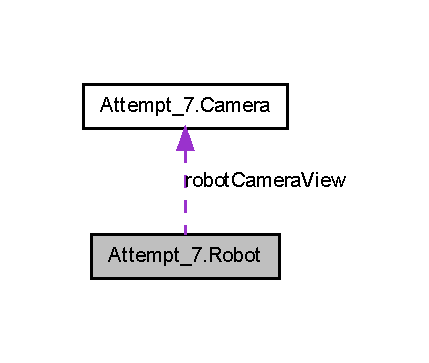
\includegraphics[width=206pt]{class_attempt__7_1_1_robot__coll__graph}
\end{center}
\end{figure}
\subsection*{Public Member Functions}
\begin{DoxyCompactItemize}
\item 
{\bf Robot} (Game game, Vector3 {\bf position}, Vector3 {\bf direction}, float {\bf speed}, float howFarToLookInFront, float {\bf cameraHeight})
\begin{DoxyCompactList}\small\item\em Initializes a new instance of the \doxyref{Robot}{p.}{class_attempt__7_1_1_robot} class. \item\end{DoxyCompactList}\item 
Vector3 {\bf GetPosition} ()
\begin{DoxyCompactList}\small\item\em Gets the current position of the \doxyref{Robot}{p.}{class_attempt__7_1_1_robot}. \item\end{DoxyCompactList}\item 
void {\bf SetPosition} (Vector3 pos)
\begin{DoxyCompactList}\small\item\em Sets the position of the robot. \item\end{DoxyCompactList}\item 
void {\bf SetStartPosition} (Vector3 pos)
\begin{DoxyCompactList}\small\item\em Called when the robot is first placed. Stores the value of the start position so that the robot can be reset to this location. \item\end{DoxyCompactList}\item 
{\bf Camera} {\bf GetRobotCamera} ()
\begin{DoxyCompactList}\small\item\em Gets the camera/view that the robot's camera sees. \item\end{DoxyCompactList}\item 
bool {\bf GetIsRobotPaused} ()
\begin{DoxyCompactList}\small\item\em Accessor method that tells if the robot is moving forward. \item\end{DoxyCompactList}\item 
Vector3 {\bf GetDirection} ()
\begin{DoxyCompactList}\small\item\em Accessor method that tells the direction the robot is going. \item\end{DoxyCompactList}\item 
override void {\bf Initialize} ()
\begin{DoxyCompactList}\small\item\em Called when the robot object is first made. The robot starts paused. \item\end{DoxyCompactList}\item 
void {\bf ChangeDirection} (float turnIndicator)
\begin{DoxyCompactList}\small\item\em Turns the robot based on the value of the turnIndicator Turn indicator must be greater or less than the threshold turn value before the robot will turn. Positive cross product of positive z with the dirrection the robot is going = \char`\"{}right\char`\"{} Negative cross product of positive z with the dirrection the robot is going = \char`\"{}left\char`\"{} \item\end{DoxyCompactList}\item 
override void {\bf Update} (GameTime gameTime)
\begin{DoxyCompactList}\small\item\em Main Update method. Calls all other methods for updating the robot. Because the robot is a GameComponent, the update method is called by the Game1.update method. \item\end{DoxyCompactList}\end{DoxyCompactItemize}
\subsection*{Protected Member Functions}
\begin{DoxyCompactItemize}
\item 
void {\bf GetKeyBoard} (GameTime gameTime1)
\begin{DoxyCompactList}\small\item\em Checks to see if a key was pressed. F1,F2,Numpad4,NumPad6,NumPad8,NumPad2 are all checked. Called by update. \item\end{DoxyCompactList}\end{DoxyCompactItemize}
\subsection*{Private Attributes}
\begin{DoxyCompactItemize}
\item 
Vector3 {\bf position}
\begin{DoxyCompactList}\small\item\em Position of the robot. \item\end{DoxyCompactList}\item 
Vector3 {\bf startPosition}
\begin{DoxyCompactList}\small\item\em Where the robot starts. Needed so it can be reset. \item\end{DoxyCompactList}\item 
Vector3 {\bf direction}
\begin{DoxyCompactList}\small\item\em Direction the robot is heading. \item\end{DoxyCompactList}\item 
float {\bf speed}
\begin{DoxyCompactList}\small\item\em Speed the robot is moving forward on update. /. \item\end{DoxyCompactList}\item 
float {\bf distanceToCameraTarget}
\begin{DoxyCompactList}\small\item\em The distance in front of the robot that the camera is pointed at. \item\end{DoxyCompactList}\item 
float {\bf cameraHeight}
\begin{DoxyCompactList}\small\item\em Height of the camera above the robot. \item\end{DoxyCompactList}\item 
{\bf Camera} {\bf robotCameraView}
\begin{DoxyCompactList}\small\item\em \doxyref{Camera}{p.}{class_attempt__7_1_1_camera} associated with the robot. \item\end{DoxyCompactList}\item 
bool {\bf paused}
\begin{DoxyCompactList}\small\item\em Is the robot moving on each all to update? if paused = true then moving, if false then not moving. \item\end{DoxyCompactList}\item 
int {\bf changeDirectionThreshholdValue} = 10
\begin{DoxyCompactList}\small\item\em How big does the turn indicator have to be, before the robot turns. 20 is default. \item\end{DoxyCompactList}\item 
int {\bf timePressedKey}
\begin{DoxyCompactList}\small\item\em Time in total milliseconds from the start of the game to the last time one of the keys was pressed. \item\end{DoxyCompactList}\end{DoxyCompactItemize}


\subsection{Detailed Description}
\doxyref{Robot}{p.}{class_attempt__7_1_1_robot} object that inherits from the XNA game component class. 

Definition at line 23 of file Robot.cs.



\subsection{Constructor \& Destructor Documentation}
\index{Attempt\_\-7::Robot@{Attempt\_\-7::Robot}!Robot@{Robot}}
\index{Robot@{Robot}!Attempt_7::Robot@{Attempt\_\-7::Robot}}
\subsubsection[{Robot}]{\setlength{\rightskip}{0pt plus 5cm}Attempt\_\-7.Robot.Robot (
\begin{DoxyParamCaption}
\item[{Game}]{game, }
\item[{Vector3}]{position, }
\item[{Vector3}]{direction, }
\item[{float}]{speed, }
\item[{float}]{howFarToLookInFront, }
\item[{float}]{cameraHeight}
\end{DoxyParamCaption}
)}\label{class_attempt__7_1_1_robot_a785ba173cf0504dee326170d3b4db554}


Initializes a new instance of the \doxyref{Robot}{p.}{class_attempt__7_1_1_robot} class. 


\begin{DoxyParams}{Parameters}
{\em game} & The game associate with the robot. \\
\hline
{\em position} & Where the robot is to start\\
\hline
{\em direction} & What direction the robot is pointed at \\
\hline
{\em speed} & How fast the robot will go. \\
\hline
{\em howFarToLookInFront} & How far in front of the robot the camera is to point. \\
\hline
{\em cameraHeight} & How high above the ground the camera for the robot is.\\
\hline
\end{DoxyParams}


Definition at line 84 of file Robot.cs.


\begin{DoxyCode}
            : base(game)
        {
            // Set the variables
            this.position = position;
            this.direction = direction;
            this.direction.Normalize();
            this.speed = speed;
            this.distanceToCameraTarget = howFarToLookInFront;
            this.cameraHeight = cameraHeight;

            // Create the camera for the robot based on the information just assi
      gned to the robot. 
            this.robotCameraView = new Camera(Game, this.position + new Vector3(0
      , 0, this.cameraHeight), this.position + Vector3.Multiply(this.direction, this.di
      stanceToCameraTarget), Vector3.Backward, false);
        }
\end{DoxyCode}


\subsection{Member Function Documentation}
\index{Attempt\_\-7::Robot@{Attempt\_\-7::Robot}!ChangeDirection@{ChangeDirection}}
\index{ChangeDirection@{ChangeDirection}!Attempt_7::Robot@{Attempt\_\-7::Robot}}
\subsubsection[{ChangeDirection}]{\setlength{\rightskip}{0pt plus 5cm}void Attempt\_\-7.Robot.ChangeDirection (
\begin{DoxyParamCaption}
\item[{float}]{turnIndicator}
\end{DoxyParamCaption}
)}\label{class_attempt__7_1_1_robot_a2ad0f76fceb915c1f1b0b98f4dc4686e}


Turns the robot based on the value of the turnIndicator Turn indicator must be greater or less than the threshold turn value before the robot will turn. Positive cross product of positive z with the dirrection the robot is going = \char`\"{}right\char`\"{} Negative cross product of positive z with the dirrection the robot is going = \char`\"{}left\char`\"{} 


\begin{DoxyParams}{Parameters}
{\em turnIndicator} & The TurnIndicator value must be passed to this method\\
\hline
\end{DoxyParams}


Definition at line 172 of file Robot.cs.


\begin{DoxyCode}
        {
            if (turnIndicator > this.changeDirectionThreshholdValue || turnIndica
      tor < -this.changeDirectionThreshholdValue)
            {
                this.direction += (Vector3.Cross(this.direction, Vector3.UnitZ) /
       2500) * turnIndicator; // 2500 is just an experimental value that works
                this.direction.Normalize(); // Make a unit vector
            }
        }
\end{DoxyCode}


Here is the caller graph for this function:\nopagebreak
\begin{figure}[H]
\begin{center}
\leavevmode
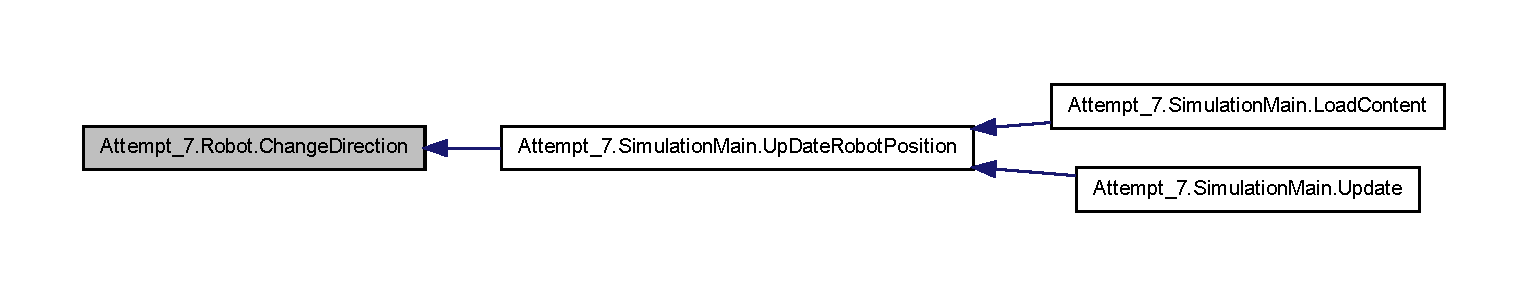
\includegraphics[width=400pt]{class_attempt__7_1_1_robot_a2ad0f76fceb915c1f1b0b98f4dc4686e_icgraph}
\end{center}
\end{figure}


\index{Attempt\_\-7::Robot@{Attempt\_\-7::Robot}!GetDirection@{GetDirection}}
\index{GetDirection@{GetDirection}!Attempt_7::Robot@{Attempt\_\-7::Robot}}
\subsubsection[{GetDirection}]{\setlength{\rightskip}{0pt plus 5cm}Vector3 Attempt\_\-7.Robot.GetDirection (
\begin{DoxyParamCaption}
{}
\end{DoxyParamCaption}
)}\label{class_attempt__7_1_1_robot_a7f204250cb4974ce920c698ce72556d8}


Accessor method that tells the direction the robot is going. 

\begin{DoxyReturn}{Returns}
Vector3 of the direction the robot is pointed
\end{DoxyReturn}


Definition at line 149 of file Robot.cs.


\begin{DoxyCode}
        {
            return this.direction;
        }
\end{DoxyCode}
\index{Attempt\_\-7::Robot@{Attempt\_\-7::Robot}!GetIsRobotPaused@{GetIsRobotPaused}}
\index{GetIsRobotPaused@{GetIsRobotPaused}!Attempt_7::Robot@{Attempt\_\-7::Robot}}
\subsubsection[{GetIsRobotPaused}]{\setlength{\rightskip}{0pt plus 5cm}bool Attempt\_\-7.Robot.GetIsRobotPaused (
\begin{DoxyParamCaption}
{}
\end{DoxyParamCaption}
)}\label{class_attempt__7_1_1_robot_a68c2627772051c07f1551c38daf9ab95}


Accessor method that tells if the robot is moving forward. 

\begin{DoxyReturn}{Returns}
True if paused, false if robot is moving. 
\end{DoxyReturn}


Definition at line 140 of file Robot.cs.


\begin{DoxyCode}
        {
            return this.paused;
        }
\end{DoxyCode}


Here is the caller graph for this function:\nopagebreak
\begin{figure}[H]
\begin{center}
\leavevmode
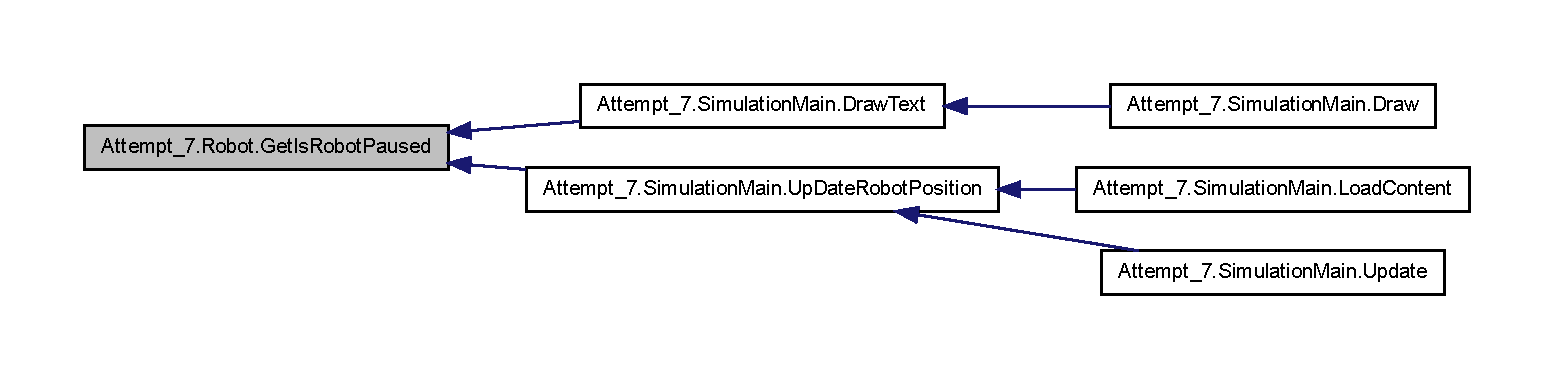
\includegraphics[width=400pt]{class_attempt__7_1_1_robot_a68c2627772051c07f1551c38daf9ab95_icgraph}
\end{center}
\end{figure}


\index{Attempt\_\-7::Robot@{Attempt\_\-7::Robot}!GetKeyBoard@{GetKeyBoard}}
\index{GetKeyBoard@{GetKeyBoard}!Attempt_7::Robot@{Attempt\_\-7::Robot}}
\subsubsection[{GetKeyBoard}]{\setlength{\rightskip}{0pt plus 5cm}void Attempt\_\-7.Robot.GetKeyBoard (
\begin{DoxyParamCaption}
\item[{GameTime}]{gameTime1}
\end{DoxyParamCaption}
)\hspace{0.3cm}{\ttfamily  [protected]}}\label{class_attempt__7_1_1_robot_a26d9c782d2b45cea22c9214cddd65e64}


Checks to see if a key was pressed. F1,F2,Numpad4,NumPad6,NumPad8,NumPad2 are all checked. Called by update. 


\begin{DoxyParams}{Parameters}
{\em gameTime1} & Clock information\\
\hline
\end{DoxyParams}


Definition at line 206 of file Robot.cs.


\begin{DoxyCode}
        {
            KeyboardState keyboardState = Keyboard.GetState();

            // Toggle pausing the game. Force 500 milliseconds between toggles. 
            if (keyboardState.IsKeyDown(Keys.F2) && gameTime1.TotalGameTime.Total
      Milliseconds - this.timePressedKey > 500)
            {
                this.timePressedKey = (int)gameTime1.TotalGameTime.TotalMilliseco
      nds;
                if (this.paused == false)
                {
                    this.paused = true;
                }
                else
                {
                    this.paused = false;
                }
            }

            // Reset the robot. 
            if (keyboardState.IsKeyDown(Keys.F1) == true)
            {
                this.position = this.startPosition;
            }

            // Turn left
            if (keyboardState.IsKeyDown(Keys.S) == true)
            {
                this.direction -= Vector3.Cross(this.direction, Vector3.UnitZ) / 
      60;
                this.direction.Normalize(); // Make a unit vector
            }

            // Turn right
            if (keyboardState.IsKeyDown(Keys.F) == true)
            {
                this.direction += Vector3.Cross(this.direction, Vector3.UnitZ) / 
      60;
                this.direction.Normalize();
            }

            // Change speed faster
            if (keyboardState.IsKeyDown(Keys.E) == true)
            {
                this.speed += 0.0001f;
            }

            // Change speed slower
            if (keyboardState.IsKeyDown(Keys.D) == true)
            {
                this.speed -= 0.0001f;
            }
        }
\end{DoxyCode}


Here is the caller graph for this function:\nopagebreak
\begin{figure}[H]
\begin{center}
\leavevmode
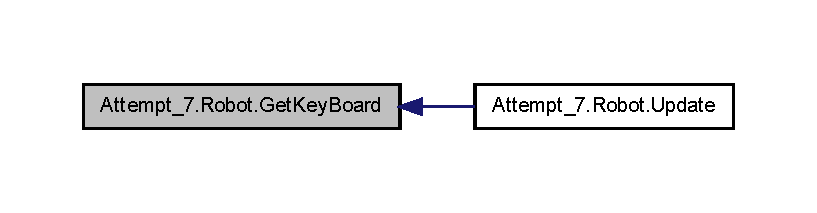
\includegraphics[width=392pt]{class_attempt__7_1_1_robot_a26d9c782d2b45cea22c9214cddd65e64_icgraph}
\end{center}
\end{figure}


\index{Attempt\_\-7::Robot@{Attempt\_\-7::Robot}!GetPosition@{GetPosition}}
\index{GetPosition@{GetPosition}!Attempt_7::Robot@{Attempt\_\-7::Robot}}
\subsubsection[{GetPosition}]{\setlength{\rightskip}{0pt plus 5cm}Vector3 Attempt\_\-7.Robot.GetPosition (
\begin{DoxyParamCaption}
{}
\end{DoxyParamCaption}
)}\label{class_attempt__7_1_1_robot_a121c5b23a88c3a1b57bbfc728e63f7bf}


Gets the current position of the \doxyref{Robot}{p.}{class_attempt__7_1_1_robot}. 

\begin{DoxyReturn}{Returns}
Vector3 value of the robot position
\end{DoxyReturn}


Definition at line 103 of file Robot.cs.


\begin{DoxyCode}
        {
            return this.position;
        }
\end{DoxyCode}


Here is the caller graph for this function:\nopagebreak
\begin{figure}[H]
\begin{center}
\leavevmode
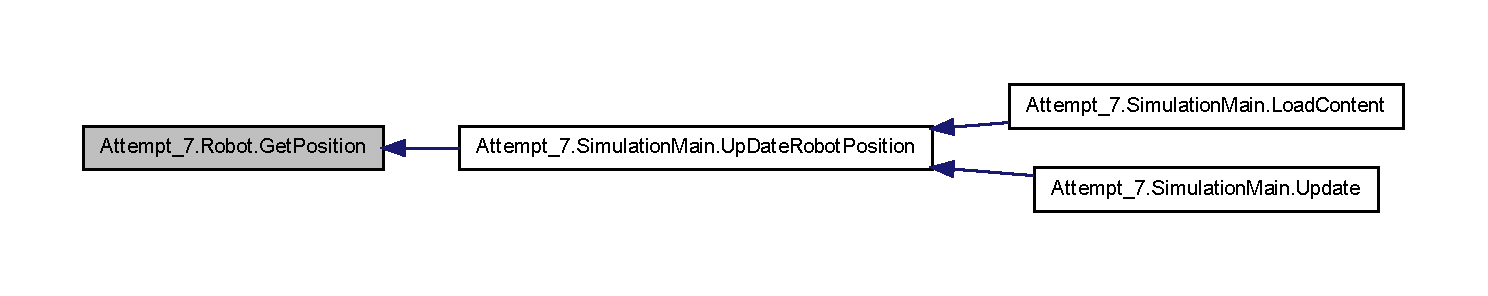
\includegraphics[width=400pt]{class_attempt__7_1_1_robot_a121c5b23a88c3a1b57bbfc728e63f7bf_icgraph}
\end{center}
\end{figure}


\index{Attempt\_\-7::Robot@{Attempt\_\-7::Robot}!GetRobotCamera@{GetRobotCamera}}
\index{GetRobotCamera@{GetRobotCamera}!Attempt_7::Robot@{Attempt\_\-7::Robot}}
\subsubsection[{GetRobotCamera}]{\setlength{\rightskip}{0pt plus 5cm}{\bf Camera} Attempt\_\-7.Robot.GetRobotCamera (
\begin{DoxyParamCaption}
{}
\end{DoxyParamCaption}
)}\label{class_attempt__7_1_1_robot_aeda683933e67246b4e3758d8bdd250c3}


Gets the camera/view that the robot's camera sees. 

\begin{DoxyReturn}{Returns}
The camera associated with the robot. 
\end{DoxyReturn}


Definition at line 131 of file Robot.cs.


\begin{DoxyCode}
        {
            return this.robotCameraView;
        }
\end{DoxyCode}


Here is the caller graph for this function:\nopagebreak
\begin{figure}[H]
\begin{center}
\leavevmode
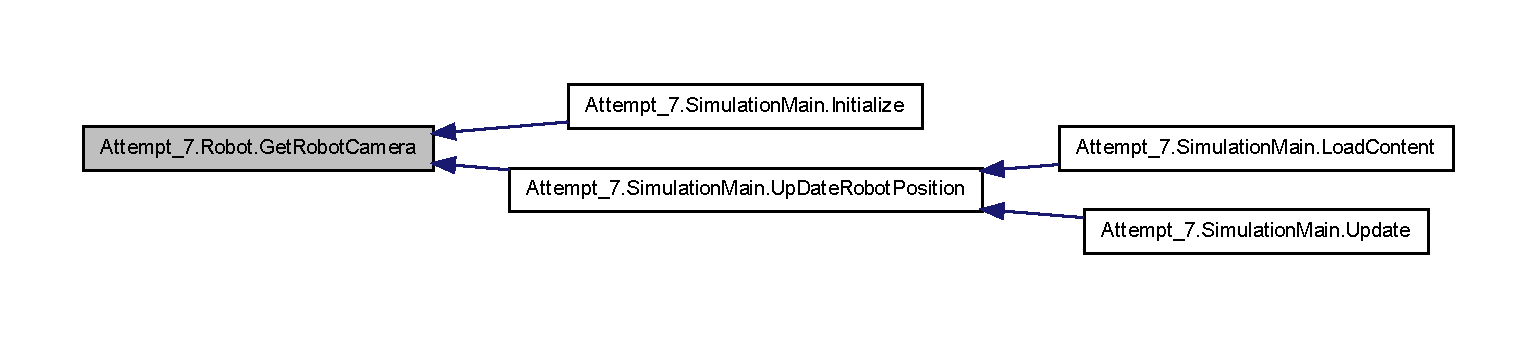
\includegraphics[width=400pt]{class_attempt__7_1_1_robot_aeda683933e67246b4e3758d8bdd250c3_icgraph}
\end{center}
\end{figure}


\index{Attempt\_\-7::Robot@{Attempt\_\-7::Robot}!Initialize@{Initialize}}
\index{Initialize@{Initialize}!Attempt_7::Robot@{Attempt\_\-7::Robot}}
\subsubsection[{Initialize}]{\setlength{\rightskip}{0pt plus 5cm}override void Attempt\_\-7.Robot.Initialize (
\begin{DoxyParamCaption}
{}
\end{DoxyParamCaption}
)}\label{class_attempt__7_1_1_robot_a4b7de5f5731480e25f70c0177495e635}


Called when the robot object is first made. The robot starts paused. 



Definition at line 158 of file Robot.cs.


\begin{DoxyCode}
        {
            this.paused = true;
            base.Initialize();
        }
\end{DoxyCode}
\index{Attempt\_\-7::Robot@{Attempt\_\-7::Robot}!SetPosition@{SetPosition}}
\index{SetPosition@{SetPosition}!Attempt_7::Robot@{Attempt\_\-7::Robot}}
\subsubsection[{SetPosition}]{\setlength{\rightskip}{0pt plus 5cm}void Attempt\_\-7.Robot.SetPosition (
\begin{DoxyParamCaption}
\item[{Vector3}]{pos}
\end{DoxyParamCaption}
)}\label{class_attempt__7_1_1_robot_a9541d93ce48fe779926507f5b0a9f229}


Sets the position of the robot. 


\begin{DoxyParams}{Parameters}
{\em pos} & The new position of the robot.\\
\hline
\end{DoxyParams}


Definition at line 112 of file Robot.cs.


\begin{DoxyCode}
        {
            this.position = pos;
        }
\end{DoxyCode}
\index{Attempt\_\-7::Robot@{Attempt\_\-7::Robot}!SetStartPosition@{SetStartPosition}}
\index{SetStartPosition@{SetStartPosition}!Attempt_7::Robot@{Attempt\_\-7::Robot}}
\subsubsection[{SetStartPosition}]{\setlength{\rightskip}{0pt plus 5cm}void Attempt\_\-7.Robot.SetStartPosition (
\begin{DoxyParamCaption}
\item[{Vector3}]{pos}
\end{DoxyParamCaption}
)}\label{class_attempt__7_1_1_robot_a9945c6d5a6e824f9669b3e6720f644e3}


Called when the robot is first placed. Stores the value of the start position so that the robot can be reset to this location. 


\begin{DoxyParams}{Parameters}
{\em pos} & The position of the robot when it starts. \\
\hline
\end{DoxyParams}


Definition at line 121 of file Robot.cs.


\begin{DoxyCode}
        {
            this.position = pos;
            this.startPosition = pos; // Set the Start position so it can be rese
      t later. 
        }
\end{DoxyCode}


Here is the caller graph for this function:\nopagebreak
\begin{figure}[H]
\begin{center}
\leavevmode
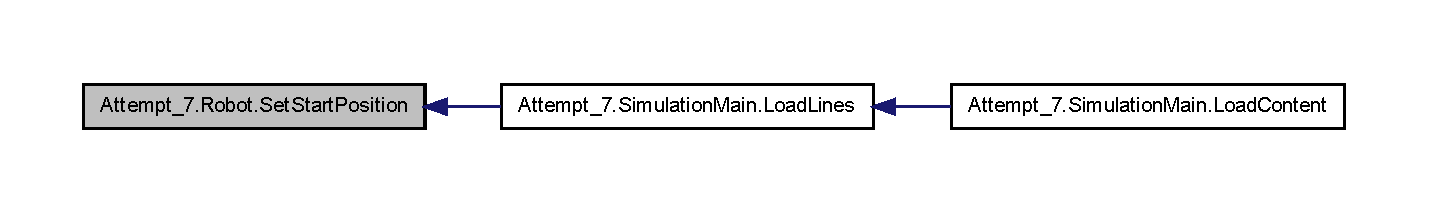
\includegraphics[width=400pt]{class_attempt__7_1_1_robot_a9945c6d5a6e824f9669b3e6720f644e3_icgraph}
\end{center}
\end{figure}


\index{Attempt\_\-7::Robot@{Attempt\_\-7::Robot}!Update@{Update}}
\index{Update@{Update}!Attempt_7::Robot@{Attempt\_\-7::Robot}}
\subsubsection[{Update}]{\setlength{\rightskip}{0pt plus 5cm}override void Attempt\_\-7.Robot.Update (
\begin{DoxyParamCaption}
\item[{GameTime}]{gameTime}
\end{DoxyParamCaption}
)}\label{class_attempt__7_1_1_robot_a4643dee9895d602aa0257eebb09fa82a}


Main Update method. Calls all other methods for updating the robot. Because the robot is a GameComponent, the update method is called by the Game1.update method. 


\begin{DoxyParams}{Parameters}
{\em gameTime} & Clock information\\
\hline
\end{DoxyParams}


Definition at line 187 of file Robot.cs.


\begin{DoxyCode}
        {
            this.GetKeyBoard(gameTime); // Get the key board values. 
            if (this.paused != true)
            {
                this.position += Vector3.Multiply(this.direction, this.speed); //
       Move the robot forward by the speed of the robot
            }

            // Set the robot camera based on its new position
            this.robotCameraView.SetCameraPositionAndTarget(this.position + new V
      ector3(0, 0, this.cameraHeight), this.position + Vector3.Multiply(this.direction,
       this.distanceToCameraTarget)); // Update the camera position
            this.robotCameraView.Update(gameTime); // Update the camera, by calli
      ng the camera's update method
            base.Update(gameTime);
        }
\end{DoxyCode}


Here is the call graph for this function:\nopagebreak
\begin{figure}[H]
\begin{center}
\leavevmode
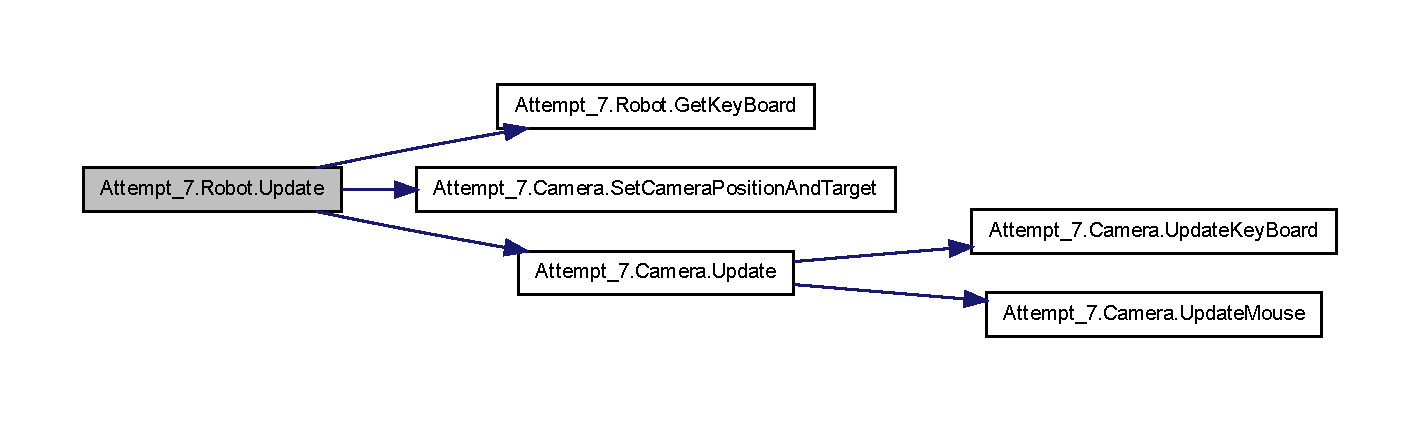
\includegraphics[width=400pt]{class_attempt__7_1_1_robot_a4643dee9895d602aa0257eebb09fa82a_cgraph}
\end{center}
\end{figure}




\subsection{Member Data Documentation}
\index{Attempt\_\-7::Robot@{Attempt\_\-7::Robot}!cameraHeight@{cameraHeight}}
\index{cameraHeight@{cameraHeight}!Attempt_7::Robot@{Attempt\_\-7::Robot}}
\subsubsection[{cameraHeight}]{\setlength{\rightskip}{0pt plus 5cm}float {\bf Attempt\_\-7.Robot.cameraHeight}\hspace{0.3cm}{\ttfamily  [private]}}\label{class_attempt__7_1_1_robot_a4f546940b473ee32465833ddb9e14bc0}


Height of the camera above the robot. 



Definition at line 53 of file Robot.cs.

\index{Attempt\_\-7::Robot@{Attempt\_\-7::Robot}!changeDirectionThreshholdValue@{changeDirectionThreshholdValue}}
\index{changeDirectionThreshholdValue@{changeDirectionThreshholdValue}!Attempt_7::Robot@{Attempt\_\-7::Robot}}
\subsubsection[{changeDirectionThreshholdValue}]{\setlength{\rightskip}{0pt plus 5cm}int {\bf Attempt\_\-7.Robot.changeDirectionThreshholdValue} = 10\hspace{0.3cm}{\ttfamily  [private]}}\label{class_attempt__7_1_1_robot_ab4f37d2ec38b3a9fa404e6d9c74c54cc}


How big does the turn indicator have to be, before the robot turns. 20 is default. 



Definition at line 68 of file Robot.cs.

\index{Attempt\_\-7::Robot@{Attempt\_\-7::Robot}!direction@{direction}}
\index{direction@{direction}!Attempt_7::Robot@{Attempt\_\-7::Robot}}
\subsubsection[{direction}]{\setlength{\rightskip}{0pt plus 5cm}Vector3 {\bf Attempt\_\-7.Robot.direction}\hspace{0.3cm}{\ttfamily  [private]}}\label{class_attempt__7_1_1_robot_aeab9c7a5393e1b353f90e179815d1d28}


Direction the robot is heading. 



Definition at line 38 of file Robot.cs.

\index{Attempt\_\-7::Robot@{Attempt\_\-7::Robot}!distanceToCameraTarget@{distanceToCameraTarget}}
\index{distanceToCameraTarget@{distanceToCameraTarget}!Attempt_7::Robot@{Attempt\_\-7::Robot}}
\subsubsection[{distanceToCameraTarget}]{\setlength{\rightskip}{0pt plus 5cm}float {\bf Attempt\_\-7.Robot.distanceToCameraTarget}\hspace{0.3cm}{\ttfamily  [private]}}\label{class_attempt__7_1_1_robot_a3d145c2fa647a421cebd0cd1ba2908e0}


The distance in front of the robot that the camera is pointed at. 



Definition at line 48 of file Robot.cs.

\index{Attempt\_\-7::Robot@{Attempt\_\-7::Robot}!paused@{paused}}
\index{paused@{paused}!Attempt_7::Robot@{Attempt\_\-7::Robot}}
\subsubsection[{paused}]{\setlength{\rightskip}{0pt plus 5cm}bool {\bf Attempt\_\-7.Robot.paused}\hspace{0.3cm}{\ttfamily  [private]}}\label{class_attempt__7_1_1_robot_a150306a7cb29e38e31b4c583dd260845}


Is the robot moving on each all to update? if paused = true then moving, if false then not moving. 



Definition at line 63 of file Robot.cs.

\index{Attempt\_\-7::Robot@{Attempt\_\-7::Robot}!position@{position}}
\index{position@{position}!Attempt_7::Robot@{Attempt\_\-7::Robot}}
\subsubsection[{position}]{\setlength{\rightskip}{0pt plus 5cm}Vector3 {\bf Attempt\_\-7.Robot.position}\hspace{0.3cm}{\ttfamily  [private]}}\label{class_attempt__7_1_1_robot_a2c385dd8076a962677e83ad6a6dc2bba}


Position of the robot. 



Definition at line 28 of file Robot.cs.

\index{Attempt\_\-7::Robot@{Attempt\_\-7::Robot}!robotCameraView@{robotCameraView}}
\index{robotCameraView@{robotCameraView}!Attempt_7::Robot@{Attempt\_\-7::Robot}}
\subsubsection[{robotCameraView}]{\setlength{\rightskip}{0pt plus 5cm}{\bf Camera} {\bf Attempt\_\-7.Robot.robotCameraView}\hspace{0.3cm}{\ttfamily  [private]}}\label{class_attempt__7_1_1_robot_a7a9896ed9d9a0eff3a72a38d9a79e16d}


\doxyref{Camera}{p.}{class_attempt__7_1_1_camera} associated with the robot. 



Definition at line 58 of file Robot.cs.

\index{Attempt\_\-7::Robot@{Attempt\_\-7::Robot}!speed@{speed}}
\index{speed@{speed}!Attempt_7::Robot@{Attempt\_\-7::Robot}}
\subsubsection[{speed}]{\setlength{\rightskip}{0pt plus 5cm}float {\bf Attempt\_\-7.Robot.speed}\hspace{0.3cm}{\ttfamily  [private]}}\label{class_attempt__7_1_1_robot_a7bf6f1325eee035a51c8ab387e7a79b8}


Speed the robot is moving forward on update. /. 



Definition at line 43 of file Robot.cs.

\index{Attempt\_\-7::Robot@{Attempt\_\-7::Robot}!startPosition@{startPosition}}
\index{startPosition@{startPosition}!Attempt_7::Robot@{Attempt\_\-7::Robot}}
\subsubsection[{startPosition}]{\setlength{\rightskip}{0pt plus 5cm}Vector3 {\bf Attempt\_\-7.Robot.startPosition}\hspace{0.3cm}{\ttfamily  [private]}}\label{class_attempt__7_1_1_robot_aa928880825b2dadef2602204a6998854}


Where the robot starts. Needed so it can be reset. 



Definition at line 33 of file Robot.cs.

\index{Attempt\_\-7::Robot@{Attempt\_\-7::Robot}!timePressedKey@{timePressedKey}}
\index{timePressedKey@{timePressedKey}!Attempt_7::Robot@{Attempt\_\-7::Robot}}
\subsubsection[{timePressedKey}]{\setlength{\rightskip}{0pt plus 5cm}int {\bf Attempt\_\-7.Robot.timePressedKey}\hspace{0.3cm}{\ttfamily  [private]}}\label{class_attempt__7_1_1_robot_a6cce884644ea640990454230965f80c5}


Time in total milliseconds from the start of the game to the last time one of the keys was pressed. 



Definition at line 73 of file Robot.cs.



The documentation for this class was generated from the following file:\begin{DoxyCompactItemize}
\item 
C:/Users/Anthony/Dropbox/Senior Project/attempt 7/attempt 7/attempt 7/{\bf Robot.cs}\end{DoxyCompactItemize}

\section{Attempt\_\-7.SimulationMain Class Reference}
\label{class_attempt__7_1_1_simulation_main}\index{Attempt\_\-7::SimulationMain@{Attempt\_\-7::SimulationMain}}


This is the main type for the Simulation.  




Collaboration diagram for Attempt\_\-7.SimulationMain:\nopagebreak
\begin{figure}[H]
\begin{center}
\leavevmode
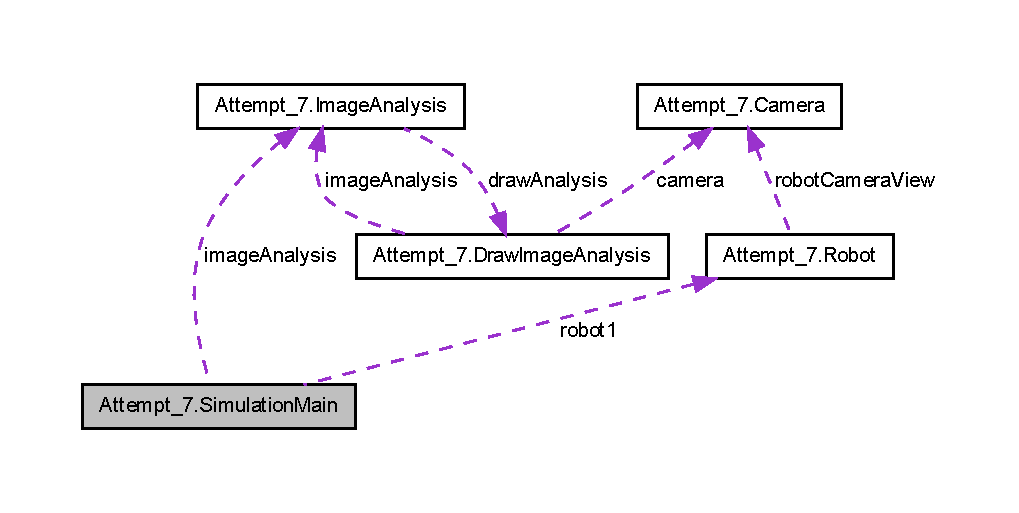
\includegraphics[width=400pt]{class_attempt__7_1_1_simulation_main__coll__graph}
\end{center}
\end{figure}
\subsection*{Public Member Functions}
\begin{DoxyCompactItemize}
\item 
{\bf SimulationMain} ()
\end{DoxyCompactItemize}
\subsection*{Static Public Attributes}
\begin{DoxyCompactItemize}
\item 
static int {\bf currentHoughMode} = 1
\begin{DoxyCompactList}\small\item\em If 0 then Old mode (top left origin), if 1 then New Hough mode( bottom Center). \item\end{DoxyCompactList}\end{DoxyCompactItemize}
\subsection*{Protected Member Functions}
\begin{DoxyCompactItemize}
\item 
override void {\bf Initialize} ()
\begin{DoxyCompactList}\small\item\em Initialize the Simulation Object. \item\end{DoxyCompactList}\item 
override void {\bf LoadContent} ()
\begin{DoxyCompactList}\small\item\em Called after initialize. Loads the textures and calls methods to create the simulated enviroment. \item\end{DoxyCompactList}\item 
override void {\bf UnloadContent} ()
\begin{DoxyCompactList}\small\item\em Unloads Information when the simulation is closed. Currently no information is saved when the simulation is closed. \item\end{DoxyCompactList}\item 
override void {\bf Update} (GameTime gameTime)
\begin{DoxyCompactList}\small\item\em Main update method for the entire simulation. Simulation logic is updated when this method is called. Part of the game loop. \item\end{DoxyCompactList}\item 
void {\bf GetKeyBoard} (GameTime gameTime1)
\begin{DoxyCompactList}\small\item\em Checks the keyboard for F3, and Escape. \item\end{DoxyCompactList}\item 
override void {\bf Draw} (GameTime gameTime)
\begin{DoxyCompactList}\small\item\em Main draw method for the simulation. Draws all the world from both the mainview and the robots view. 

The render target must be built and disposed each time or else the a memory overload will occur. \item\end{DoxyCompactList}\end{DoxyCompactItemize}
\subsection*{Private Member Functions}
\begin{DoxyCompactItemize}
\item 
void {\bf DrawTextDebugInfo} ()
\item 
void {\bf CreateViewPorts} ()
\begin{DoxyCompactList}\small\item\em Creates the 5 view ports. View ports are like windows inside of a Window's window. 
\begin{DoxyItemize}
\item MainPort = 0  
\item TopRight = 1 
\item CenterRight = 2 
\item BottomRight = 3 
\item BottomLeft = 4 
\item BottomCenter = 5 
\end{DoxyItemize}\item\end{DoxyCompactList}\item 
Texture2D {\bf CreateGrassTexture} (Texture2D texturetoUse)
\begin{DoxyCompactList}\small\item\em Takes a texture and returns a larger texture. Size of the new texture is 1024,1024. \item\end{DoxyCompactList}\item 
Color[,] {\bf TextureTo2DArray} (Texture2D texture)
\begin{DoxyCompactList}\small\item\em Takes a texture converts it into a 2D color array. \item\end{DoxyCompactList}\item 
void {\bf LoadGround} ()
\begin{DoxyCompactList}\small\item\em Create vertex data for the grass. Verts2 is the VertexPositionTexture array. \item\end{DoxyCompactList}\item 
void {\bf LoadLines} ()
\begin{DoxyCompactList}\small\item\em Creates the vertexPositionColor array \char`\"{}verts1\char`\"{} that is used to draw the white lines. \item\end{DoxyCompactList}\item 
void {\bf UpDateRobotPosition} ()
\begin{DoxyCompactList}\small\item\em Loads the vertex information about the robot and recreates it every game cycle to reflect the new position of the robot. 'verts3' is the VertexPositionColor array. \item\end{DoxyCompactList}\item 
void {\bf BuildRenderTargets} ()
\begin{DoxyCompactList}\small\item\em Set the renderTargets to a texture object in memory rather than rendering to the screen. Need target for both the Worldview and the robot CameraView. \item\end{DoxyCompactList}\item 
void {\bf DrawRobot} ({\bf Camera} camera)
\begin{DoxyCompactList}\small\item\em Draw the robot from the \char`\"{}camera\char`\"{}s perspective. \item\end{DoxyCompactList}\item 
void {\bf DrawColorLines} ({\bf Camera} camera)
\begin{DoxyCompactList}\small\item\em Draw the lines from the \char`\"{}camera\char`\"{}'s persepective. \item\end{DoxyCompactList}\item 
void {\bf DrawGrass} ({\bf Camera} camera)
\begin{DoxyCompactList}\small\item\em Draw the grass or ground from \char`\"{}camera\char`\"{}'s perspective. \item\end{DoxyCompactList}\item 
void {\bf DrawText} ()
\begin{DoxyCompactList}\small\item\em Draw the Simulation Status as either PAUSED or Active. \item\end{DoxyCompactList}\end{DoxyCompactItemize}
\subsection*{Private Attributes}
\begin{DoxyCompactItemize}
\item 
GraphicsDeviceManager {\bf graphics}
\begin{DoxyCompactList}\small\item\em GPU manager. \item\end{DoxyCompactList}\item 
Vector2 {\bf screenSize} = new Vector2(640, 480)
\begin{DoxyCompactList}\small\item\em 2D vector representing the resolution of the cameras used in the simulation. \item\end{DoxyCompactList}\item 
Rectangle {\bf screenRectangle} = new Rectangle(0, 0, 640, 480)
\begin{DoxyCompactList}\small\item\em Rectangle object that is the size of the camera resolution (screenSize). \item\end{DoxyCompactList}\item 
Vector2 {\bf windowSize} = new Vector2(1000, 780)
\begin{DoxyCompactList}\small\item\em 2D vector represeting the size of the Window's Window that the simulation will run in. \item\end{DoxyCompactList}\item 
SpriteBatch {\bf spriteBatch}
\begin{DoxyCompactList}\small\item\em The sprite batch object. Used to draw 2D graphics. \item\end{DoxyCompactList}\item 
Texture2D {\bf grass}
\begin{DoxyCompactList}\small\item\em Represents the texture of the grass bitmap that is used to represent the grass. \item\end{DoxyCompactList}\item 
Texture2D {\bf largeGrass}
\begin{DoxyCompactList}\small\item\em A large tiled version of the grass Texture. \item\end{DoxyCompactList}\item 
BasicEffect {\bf basicEffects}
\begin{DoxyCompactList}\small\item\em The basicEffects for rendering in 3D. \item\end{DoxyCompactList}\item 
VertexPositionColor[$\,$] {\bf verts1}
\begin{DoxyCompactList}\small\item\em The vertexPositionColor array holding the vertex information needed for drawing the white lines representing the course. \item\end{DoxyCompactList}\item 
VertexPositionTexture[$\,$] {\bf verts2}
\begin{DoxyCompactList}\small\item\em The vertexPositionColor array holding the information for the grass/ground. \item\end{DoxyCompactList}\item 
VertexPositionColor[$\,$] {\bf verts3}
\begin{DoxyCompactList}\small\item\em The vertexPositionColor Array holding the information needed for the 3D representation of the robot. \item\end{DoxyCompactList}\item 
List$<$ Viewport $>$ {\bf viewPortList}
\begin{DoxyCompactList}\small\item\em List holding the viewports used in the simulation. \item\end{DoxyCompactList}\item 
bool {\bf trackRobot} = false
\begin{DoxyCompactList}\small\item\em Bool representing if the main \doxyref{Camera}{p.}{class_attempt__7_1_1_camera} moves its view to follow the robot. \item\end{DoxyCompactList}\item 
int {\bf timePressedKey} = 0
\begin{DoxyCompactList}\small\item\em Time in totalmillseconds when F1, F2, or F3 were pushed. \item\end{DoxyCompactList}\item 
SpriteFont {\bf arialLarge}
\begin{DoxyCompactList}\small\item\em The 2D font object needed to show text. Size = 20. \item\end{DoxyCompactList}\item 
SpriteFont {\bf arialSmall}
\begin{DoxyCompactList}\small\item\em A smaller font of arial to show debug information. \item\end{DoxyCompactList}\item 
Random {\bf rand}
\begin{DoxyCompactList}\small\item\em Represents a random object so that random numbers can be generated. \item\end{DoxyCompactList}\item 
{\bf Robot} {\bf robot1}
\begin{DoxyCompactList}\small\item\em The robot object. See the robot class for more information. \item\end{DoxyCompactList}\item 
List$<$ {\bf Camera} $>$ {\bf cameraList}
\begin{DoxyCompactList}\small\item\em A list of the cameras. There are 2, The mainview and the robot view. 
\begin{DoxyItemize}
\item WorldView \doxyref{Camera}{p.}{class_attempt__7_1_1_camera} = 0 (The main camera) 
\item \doxyref{Robot}{p.}{class_attempt__7_1_1_robot} View \doxyref{Camera}{p.}{class_attempt__7_1_1_camera} = 1  
\end{DoxyItemize}\item\end{DoxyCompactList}\item 
List$<$ RenderTarget2D $>$ {\bf renderTargets}
\begin{DoxyCompactList}\small\item\em A list of the rendertargets. Rather than rendering to the screen, the image produced by the GPU is saved to a rendertarget.  The rendertargets correspond directly with the camera views.  


\begin{DoxyItemize}
\item World View Target = 0  
\item \doxyref{Robot}{p.}{class_attempt__7_1_1_robot} View Target = 1 
\end{DoxyItemize}\item\end{DoxyCompactList}\item 
{\bf ImageAnalysis} {\bf imageAnalysis}
\begin{DoxyCompactList}\small\item\em The image analysis object/class does the image processing. \item\end{DoxyCompactList}\end{DoxyCompactItemize}


\subsection{Detailed Description}
This is the main type for the Simulation. 

Definition at line 25 of file SimulationMain.cs.



\subsection{Constructor \& Destructor Documentation}
\index{Attempt\_\-7::SimulationMain@{Attempt\_\-7::SimulationMain}!SimulationMain@{SimulationMain}}
\index{SimulationMain@{SimulationMain}!Attempt_7::SimulationMain@{Attempt\_\-7::SimulationMain}}
\subsubsection[{SimulationMain}]{\setlength{\rightskip}{0pt plus 5cm}Attempt\_\-7.SimulationMain.SimulationMain (
\begin{DoxyParamCaption}
{}
\end{DoxyParamCaption}
)}\label{class_attempt__7_1_1_simulation_main_a9ea5edf642dc80c782aa35f4a4ba4107}
Initializes a new instance of the \doxyref{SimulationMain}{p.}{class_attempt__7_1_1_simulation_main} class. 

Definition at line 146 of file SimulationMain.cs.


\begin{DoxyCode}
        {
            this.graphics = new GraphicsDeviceManager(this);
            Content.RootDirectory = "Content";
        }
\end{DoxyCode}


\subsection{Member Function Documentation}
\index{Attempt\_\-7::SimulationMain@{Attempt\_\-7::SimulationMain}!BuildRenderTargets@{BuildRenderTargets}}
\index{BuildRenderTargets@{BuildRenderTargets}!Attempt_7::SimulationMain@{Attempt\_\-7::SimulationMain}}
\subsubsection[{BuildRenderTargets}]{\setlength{\rightskip}{0pt plus 5cm}void Attempt\_\-7.SimulationMain.BuildRenderTargets (
\begin{DoxyParamCaption}
{}
\end{DoxyParamCaption}
)\hspace{0.3cm}{\ttfamily  [private]}}\label{class_attempt__7_1_1_simulation_main_a596379dec8c50adc14977c75005def80}


Set the renderTargets to a texture object in memory rather than rendering to the screen. Need target for both the Worldview and the robot CameraView. 



Definition at line 528 of file SimulationMain.cs.


\begin{DoxyCode}
        {
            this.renderTargets = new List<RenderTarget2D>(); // This list will co
      rrespond to the camera list

            // Main view target. 
            RenderTarget2D targetWorldView = new RenderTarget2D(this.GraphicsDevi
      ce, (int)this.screenSize.X, (int)this.screenSize.Y); // Create a target for rende
      ring of the mouse countroled camera view
            this.renderTargets.Add(targetWorldView); // Add to the list of target
      s

            // The render target for the robot's camera view.  
            RenderTarget2D targetRobotView = new RenderTarget2D(GraphicsDevice, (
      int)this.screenSize.X, (int)this.screenSize.Y); // Create a target for the render
       of the robot camera view
            this.renderTargets.Add(targetRobotView); // Add to the list          
           
        }
\end{DoxyCode}


Here is the caller graph for this function:\nopagebreak
\begin{figure}[H]
\begin{center}
\leavevmode
\includegraphics[width=400pt]{class_attempt__7_1_1_simulation_main_a596379dec8c50adc14977c75005def80_icgraph}
\end{center}
\end{figure}


\index{Attempt\_\-7::SimulationMain@{Attempt\_\-7::SimulationMain}!CreateGrassTexture@{CreateGrassTexture}}
\index{CreateGrassTexture@{CreateGrassTexture}!Attempt_7::SimulationMain@{Attempt\_\-7::SimulationMain}}
\subsubsection[{CreateGrassTexture}]{\setlength{\rightskip}{0pt plus 5cm}Texture2D Attempt\_\-7.SimulationMain.CreateGrassTexture (
\begin{DoxyParamCaption}
\item[{Texture2D}]{texturetoUse}
\end{DoxyParamCaption}
)\hspace{0.3cm}{\ttfamily  [private]}}\label{class_attempt__7_1_1_simulation_main_a931a8a86dead3b0cb29f28453cf4f6f0}


Takes a texture and returns a larger texture. Size of the new texture is 1024,1024. 


\begin{DoxyParams}{Parameters}
{\em texturetoUse} & The smaller texture to tile\\
\hline
\end{DoxyParams}
\begin{DoxyReturn}{Returns}
The larger texture with the smaller on tiled onto it. 
\end{DoxyReturn}


Definition at line 401 of file SimulationMain.cs.


\begin{DoxyCode}
        {
            Color[,] groundColors = this.TextureTo2DArray(texturetoUse);
            Vector2 newTextureSize = new Vector2(1024, 1024); // Size of the new 
      texture. 
            Color[] foregroundColors = new Color[(int)newTextureSize.X * (int)new
      TextureSize.Y];

            for (int x = 0; x < (int)newTextureSize.X; x++)
            {
                for (int y = 0; y < (int)newTextureSize.Y; y++)
                {
                    foregroundColors[x + (y * (int)newTextureSize.X)] = groundCol
      ors[(x * 2) % texturetoUse.Width, (y * 2) % texturetoUse.Height];
                }
            }

            Texture2D newTexture = new Texture2D(this.GraphicsDevice, (int)newTex
      tureSize.X, (int)newTextureSize.Y, false, SurfaceFormat.Color);
            newTexture.SetData(foregroundColors);
            return newTexture;
        }
\end{DoxyCode}


Here is the call graph for this function:\nopagebreak
\begin{figure}[H]
\begin{center}
\leavevmode
\includegraphics[width=400pt]{class_attempt__7_1_1_simulation_main_a931a8a86dead3b0cb29f28453cf4f6f0_cgraph}
\end{center}
\end{figure}




Here is the caller graph for this function:\nopagebreak
\begin{figure}[H]
\begin{center}
\leavevmode
\includegraphics[width=400pt]{class_attempt__7_1_1_simulation_main_a931a8a86dead3b0cb29f28453cf4f6f0_icgraph}
\end{center}
\end{figure}


\index{Attempt\_\-7::SimulationMain@{Attempt\_\-7::SimulationMain}!CreateViewPorts@{CreateViewPorts}}
\index{CreateViewPorts@{CreateViewPorts}!Attempt_7::SimulationMain@{Attempt\_\-7::SimulationMain}}
\subsubsection[{CreateViewPorts}]{\setlength{\rightskip}{0pt plus 5cm}void Attempt\_\-7.SimulationMain.CreateViewPorts (
\begin{DoxyParamCaption}
{}
\end{DoxyParamCaption}
)\hspace{0.3cm}{\ttfamily  [private]}}\label{class_attempt__7_1_1_simulation_main_aabe2d52bb2b34aeeff6a5d8c98512ef6}


Creates the 5 view ports. View ports are like windows inside of a Window's window. 
\begin{DoxyItemize}
\item MainPort = 0  
\item TopRight = 1 
\item CenterRight = 2 
\item BottomRight = 3 
\item BottomLeft = 4 
\item BottomCenter = 5 
\end{DoxyItemize}



Definition at line 366 of file SimulationMain.cs.


\begin{DoxyCode}
        {
            this.viewPortList = new List<Viewport>(); // Make a list for the view
      ports

            Viewport mainView = GraphicsDevice.Viewport; // Default view port is 
      the window size. 
            mainView.Width = (int)GraphicsDevice.Viewport.Width * 2 / 3; // Takes
       up 2/3 of the x and y distances
            mainView.Height = (int)GraphicsDevice.Viewport.Height * 2 / 3;
            this.viewPortList.Add(mainView);

            for (int i = 0; i < 3; i++)
            {
                Viewport viewSide0 = GraphicsDevice.Viewport;
                viewSide0.X = (int)GraphicsDevice.Viewport.Width * 2 / 3;
                viewSide0.Y = i * (int)GraphicsDevice.Viewport.Height * 1 / 3; //
       Make 3 on the right side of the screen going down. 
                viewSide0.Width = (int)GraphicsDevice.Viewport.Width * 1 / 3;
                viewSide0.Height = (int)GraphicsDevice.Viewport.Height * 1 / 3;
                this.viewPortList.Add(viewSide0);
            }

            for (int i = 0; i < 2; i++)
            {
                Viewport viewSide0 = GraphicsDevice.Viewport;
                viewSide0.X = i * (int)GraphicsDevice.Viewport.Width * 1 / 3;
                viewSide0.Y = (int)GraphicsDevice.Viewport.Height * 2 / 3; // Mak
      e 3 on bottom of the screen going left. 
                viewSide0.Width = (int)GraphicsDevice.Viewport.Width * 1 / 3;
                viewSide0.Height = (int)GraphicsDevice.Viewport.Height * 1 / 3;
                this.viewPortList.Add(viewSide0);
            }
        }       
\end{DoxyCode}


Here is the caller graph for this function:\nopagebreak
\begin{figure}[H]
\begin{center}
\leavevmode
\includegraphics[width=400pt]{class_attempt__7_1_1_simulation_main_aabe2d52bb2b34aeeff6a5d8c98512ef6_icgraph}
\end{center}
\end{figure}


\index{Attempt\_\-7::SimulationMain@{Attempt\_\-7::SimulationMain}!Draw@{Draw}}
\index{Draw@{Draw}!Attempt_7::SimulationMain@{Attempt\_\-7::SimulationMain}}
\subsubsection[{Draw}]{\setlength{\rightskip}{0pt plus 5cm}override void Attempt\_\-7.SimulationMain.Draw (
\begin{DoxyParamCaption}
\item[{GameTime}]{gameTime}
\end{DoxyParamCaption}
)\hspace{0.3cm}{\ttfamily  [protected]}}\label{class_attempt__7_1_1_simulation_main_ae2774f61c773a44b36670c81e5df8b05}


Main draw method for the simulation. Draws all the world from both the mainview and the robots view. 

The render target must be built and disposed each time or else the a memory overload will occur. 

Each time the Viewport is changed a new spriteBatch.Start method must be called.


\begin{DoxyParams}{Parameters}
{\em gameTime} & Clock Information\\
\hline
\end{DoxyParams}


Definition at line 294 of file SimulationMain.cs.


\begin{DoxyCode}
        {
            this.BuildRenderTargets(); // Create the render targets to be in the 
      computer memory instead of the screen. 

            int h = 0;

            // Go through each camera and draw the world from its persepective. 
            foreach (Camera cam in this.cameraList) 
            {
                this.GraphicsDevice.SetRenderTarget(this.renderTargets[h]); // Se
      t the render target, worldview then robot view
                this.GraphicsDevice.Clear(Color.Black); // Clear the screen to Bl
      ack

                // Draw the world from the perspective of each camera
                this.DrawGrass(cam); // i.e grass
                this.DrawColorLines(cam);
                this.DrawRobot(cam);
                h++; // Go to the next render target
            }

            // Set the renderTarget to the scree, Clear the screen, 
            this.GraphicsDevice.SetRenderTarget(null); // Set the rendering targe
      t back to the screen
            this.GraphicsDevice.Clear(Color.Gray); // Clear the screen to Gray

            // Send the imageAnalysis object the robot's view, 
            this.imageAnalysis.SetRobotCameraView(this.renderTargets[1]); // Send
       the camera view from the robot camera to the analysis class
            this.imageAnalysis.Update1(gameTime); // Pull out the color data of t
      he texture before the texture is disposed. 

            // Draw the render target, maks sure the source rectange size is the 
      same as the texture to draw size,
            // (texture to draw, size of the part of the texture you what draw (t
      he whole thing), Color, rotation, Origin of the texture,scale to 3/4 size, no eff
      ects, 0 is default)

            // Set the view port to the main view and draw the main view
            this.GraphicsDevice.Viewport = this.viewPortList[0]; // Main View  is
       2/3 of the screen screen
            this.spriteBatch.Begin(); // Start the 2D drawing        
            this.spriteBatch.Draw(this.renderTargets[0], new Rectangle(0, 0, Grap
      hicsDevice.Viewport.Width, GraphicsDevice.Viewport.Height), Color.White); // Draw
       the MainView
            this.DrawText(); // Draw a message about whether the simulation is pa
      used or active. 
            this.spriteBatch.End(); // Stop drawing. 

            // Change viewports to the topLeft view port of the window. Draw the 
      robot view. 
            this.GraphicsDevice.Viewport = this.viewPortList[1];
            this.spriteBatch.Begin(); // Start the 2D drawing      
            this.spriteBatch.Draw(this.renderTargets[1], new Rectangle(0, 0, Grap
      hicsDevice.Viewport.Width, GraphicsDevice.Viewport.Height), Color.White); // Draw
       the robotView
            this.spriteBatch.End(); // Stop drawing.


            // Change viewports to the bottomriht view port of the window. GiveDe
      bug information. 
            this.GraphicsDevice.Viewport = this.viewPortList[4];
            this.spriteBatch.Begin(); // Start the 2D drawing     
            this.DrawTextDebugInfo();
            this.spriteBatch.End(); // Stop drawing.
           
            base.Draw(gameTime); // Call all the drawableGameCmponets draw method
       (imageAnalysis.cs).
            foreach (RenderTarget2D r in this.renderTargets)
            {
                r.Dispose(); // Free up the memory resources 
            }
        }
\end{DoxyCode}


Here is the call graph for this function:\nopagebreak
\begin{figure}[H]
\begin{center}
\leavevmode
\includegraphics[width=400pt]{class_attempt__7_1_1_simulation_main_ae2774f61c773a44b36670c81e5df8b05_cgraph}
\end{center}
\end{figure}


\index{Attempt\_\-7::SimulationMain@{Attempt\_\-7::SimulationMain}!DrawColorLines@{DrawColorLines}}
\index{DrawColorLines@{DrawColorLines}!Attempt_7::SimulationMain@{Attempt\_\-7::SimulationMain}}
\subsubsection[{DrawColorLines}]{\setlength{\rightskip}{0pt plus 5cm}void Attempt\_\-7.SimulationMain.DrawColorLines (
\begin{DoxyParamCaption}
\item[{{\bf Camera}}]{camera}
\end{DoxyParamCaption}
)\hspace{0.3cm}{\ttfamily  [private]}}\label{class_attempt__7_1_1_simulation_main_a6600ca6533a6db25d8796c13b63c1a40}


Draw the lines from the \char`\"{}camera\char`\"{}'s persepective. 


\begin{DoxyParams}{Parameters}
{\em camera} & The camera to use when drawing.\\
\hline
\end{DoxyParams}


Definition at line 564 of file SimulationMain.cs.


\begin{DoxyCode}
        {
            this.basicEffects.World = camera.World;
            this.basicEffects.View = camera.View;
            this.basicEffects.Projection = camera.Projection;
            this.basicEffects.TextureEnabled = false;
            this.basicEffects.VertexColorEnabled = true;

            foreach (EffectPass pass in this.basicEffects.CurrentTechnique.Passes
      )
            {
                pass.Apply();
                this.GraphicsDevice.DrawUserPrimitives<VertexPositionColor>(Primi
      tiveType.LineStrip, this.verts1, 0, 36); // Draw the 1st inner line
                this.GraphicsDevice.DrawUserPrimitives<VertexPositionColor>(Primi
      tiveType.LineStrip, this.verts1, 37, 36); // Draw the 2nd inner line
                this.GraphicsDevice.DrawUserPrimitives<VertexPositionColor>(Primi
      tiveType.LineStrip, this.verts1, 37 * 2, 36); // Draw the outerline
                this.GraphicsDevice.DrawUserPrimitives<VertexPositionColor>(Primi
      tiveType.LineStrip, this.verts1, 37 * 3, 36); // Draw the 2nd outerline          
           
            }
        }
\end{DoxyCode}


Here is the caller graph for this function:\nopagebreak
\begin{figure}[H]
\begin{center}
\leavevmode
\includegraphics[width=400pt]{class_attempt__7_1_1_simulation_main_a6600ca6533a6db25d8796c13b63c1a40_icgraph}
\end{center}
\end{figure}


\index{Attempt\_\-7::SimulationMain@{Attempt\_\-7::SimulationMain}!DrawGrass@{DrawGrass}}
\index{DrawGrass@{DrawGrass}!Attempt_7::SimulationMain@{Attempt\_\-7::SimulationMain}}
\subsubsection[{DrawGrass}]{\setlength{\rightskip}{0pt plus 5cm}void Attempt\_\-7.SimulationMain.DrawGrass (
\begin{DoxyParamCaption}
\item[{{\bf Camera}}]{camera}
\end{DoxyParamCaption}
)\hspace{0.3cm}{\ttfamily  [private]}}\label{class_attempt__7_1_1_simulation_main_abbd56e335ac6f87700aa78afdea7c6c8}


Draw the grass or ground from \char`\"{}camera\char`\"{}'s perspective. 


\begin{DoxyParams}{Parameters}
{\em camera} & The camera to use when drawing.\\
\hline
\end{DoxyParams}


Definition at line 586 of file SimulationMain.cs.


\begin{DoxyCode}
        {
            this.basicEffects.World = camera.World;
            this.basicEffects.View = camera.View;
            this.basicEffects.Projection = camera.Projection;
            this.basicEffects.VertexColorEnabled = false;
            this.basicEffects.Texture = this.largeGrass  ;
            this.basicEffects.TextureEnabled = true; // Because the ground is a t
      exture object. 
           

            foreach (EffectPass pass in this.basicEffects.CurrentTechnique.Passes
      )
            {
                pass.Apply();
                GraphicsDevice.DrawUserPrimitives<VertexPositionTexture>(Primitiv
      eType.TriangleStrip, this.verts2, 0, 2);
            }
        }
\end{DoxyCode}


Here is the caller graph for this function:\nopagebreak
\begin{figure}[H]
\begin{center}
\leavevmode
\includegraphics[width=400pt]{class_attempt__7_1_1_simulation_main_abbd56e335ac6f87700aa78afdea7c6c8_icgraph}
\end{center}
\end{figure}


\index{Attempt\_\-7::SimulationMain@{Attempt\_\-7::SimulationMain}!DrawRobot@{DrawRobot}}
\index{DrawRobot@{DrawRobot}!Attempt_7::SimulationMain@{Attempt\_\-7::SimulationMain}}
\subsubsection[{DrawRobot}]{\setlength{\rightskip}{0pt plus 5cm}void Attempt\_\-7.SimulationMain.DrawRobot (
\begin{DoxyParamCaption}
\item[{{\bf Camera}}]{camera}
\end{DoxyParamCaption}
)\hspace{0.3cm}{\ttfamily  [private]}}\label{class_attempt__7_1_1_simulation_main_acfd54a5aa5fb4311b2938ee7ab121022}


Draw the robot from the \char`\"{}camera\char`\"{}s perspective. 


\begin{DoxyParams}{Parameters}
{\em camera} & The camera to use when drawing. \\
\hline
\end{DoxyParams}


Definition at line 545 of file SimulationMain.cs.


\begin{DoxyCode}
        {
            this.basicEffects.World = camera.World;
            this.basicEffects.View = camera.View;
            this.basicEffects.Projection = camera.Projection;
            this.basicEffects.TextureEnabled = false;
            this.basicEffects.VertexColorEnabled = true;

            foreach (EffectPass pass in this.basicEffects.CurrentTechnique.Passes
      )
            {
                pass.Apply();
                this.GraphicsDevice.DrawUserPrimitives<VertexPositionColor>(Primi
      tiveType.TriangleStrip, this.verts3, 0, 3); // Verts3 is the robot.              
        
            }
        }
\end{DoxyCode}


Here is the caller graph for this function:\nopagebreak
\begin{figure}[H]
\begin{center}
\leavevmode
\includegraphics[width=400pt]{class_attempt__7_1_1_simulation_main_acfd54a5aa5fb4311b2938ee7ab121022_icgraph}
\end{center}
\end{figure}


\index{Attempt\_\-7::SimulationMain@{Attempt\_\-7::SimulationMain}!DrawText@{DrawText}}
\index{DrawText@{DrawText}!Attempt_7::SimulationMain@{Attempt\_\-7::SimulationMain}}
\subsubsection[{DrawText}]{\setlength{\rightskip}{0pt plus 5cm}void Attempt\_\-7.SimulationMain.DrawText (
\begin{DoxyParamCaption}
{}
\end{DoxyParamCaption}
)\hspace{0.3cm}{\ttfamily  [private]}}\label{class_attempt__7_1_1_simulation_main_aa933058eb5333dbb1addb68b72c27def}


Draw the Simulation Status as either PAUSED or Active. 



Definition at line 606 of file SimulationMain.cs.


\begin{DoxyCode}
        {
            bool simulationPause = this.robot1.GetIsRobotPaused(); // Find if the
       simulatin is paused from the robot. 

            if (simulationPause == true)
            {
                this.spriteBatch.DrawString(this.arialLarge, "Simulation Status--
      - PAUSED", new Vector2(0, 0), Color.Yellow);
            }
            else
            {
                this.spriteBatch.DrawString(this.arialLarge, "Simulation Status--
      - Active", new Vector2(0, 0), Color.Green);
            }
        }
\end{DoxyCode}


Here is the call graph for this function:\nopagebreak
\begin{figure}[H]
\begin{center}
\leavevmode
\includegraphics[width=400pt]{class_attempt__7_1_1_simulation_main_aa933058eb5333dbb1addb68b72c27def_cgraph}
\end{center}
\end{figure}




Here is the caller graph for this function:\nopagebreak
\begin{figure}[H]
\begin{center}
\leavevmode
\includegraphics[width=400pt]{class_attempt__7_1_1_simulation_main_aa933058eb5333dbb1addb68b72c27def_icgraph}
\end{center}
\end{figure}


\index{Attempt\_\-7::SimulationMain@{Attempt\_\-7::SimulationMain}!DrawTextDebugInfo@{DrawTextDebugInfo}}
\index{DrawTextDebugInfo@{DrawTextDebugInfo}!Attempt_7::SimulationMain@{Attempt\_\-7::SimulationMain}}
\subsubsection[{DrawTextDebugInfo}]{\setlength{\rightskip}{0pt plus 5cm}void Attempt\_\-7.SimulationMain.DrawTextDebugInfo (
\begin{DoxyParamCaption}
{}
\end{DoxyParamCaption}
)\hspace{0.3cm}{\ttfamily  [private]}}\label{class_attempt__7_1_1_simulation_main_afe6aa0f5c85b090b06c0228cf4e7c21c}


Definition at line 351 of file SimulationMain.cs.


\begin{DoxyCode}
        {
        }
\end{DoxyCode}


Here is the caller graph for this function:\nopagebreak
\begin{figure}[H]
\begin{center}
\leavevmode
\includegraphics[width=400pt]{class_attempt__7_1_1_simulation_main_afe6aa0f5c85b090b06c0228cf4e7c21c_icgraph}
\end{center}
\end{figure}


\index{Attempt\_\-7::SimulationMain@{Attempt\_\-7::SimulationMain}!GetKeyBoard@{GetKeyBoard}}
\index{GetKeyBoard@{GetKeyBoard}!Attempt_7::SimulationMain@{Attempt\_\-7::SimulationMain}}
\subsubsection[{GetKeyBoard}]{\setlength{\rightskip}{0pt plus 5cm}void Attempt\_\-7.SimulationMain.GetKeyBoard (
\begin{DoxyParamCaption}
\item[{GameTime}]{gameTime1}
\end{DoxyParamCaption}
)\hspace{0.3cm}{\ttfamily  [protected]}}\label{class_attempt__7_1_1_simulation_main_a4b98b01df022d9a02ce98bf80f0f5c9b}


Checks the keyboard for F3, and Escape. 


\begin{DoxyParams}{Parameters}
{\em gameTime1} & Clock information\\
\hline
\end{DoxyParams}


Definition at line 232 of file SimulationMain.cs.


\begin{DoxyCode}
        {
            KeyboardState keyboardState = Keyboard.GetState();

            // Force 500 millsecond between updates
            if (gameTime1.TotalGameTime.TotalMilliseconds - this.timePressedKey >
       500)
            {
                if (keyboardState.IsKeyDown(Keys.F3))
                {
                    this.timePressedKey = (int)gameTime1.TotalGameTime.TotalMilli
      seconds;
                    if (this.trackRobot == false)
                    {
                        this.trackRobot = true; // Toggle on and off  
                    }
                    else
                    {
                        this.trackRobot = false; // Toggle on and off  
                    }
                }

                //toggle the hough mode. 
                if (keyboardState.IsKeyDown(Keys.F4))
                {
                    this.timePressedKey = (int)gameTime1.TotalGameTime.TotalMilli
      seconds;
                    if (currentHoughMode  == 0)
                    {
                        currentHoughMode = 1; // Toggle on and off  
                    }
                    else
                    {
                        currentHoughMode = 0; // Toggle on and off  
                    }
                }
            }

            // Allows the game to exit when Escape is hit. 
            if (keyboardState.IsKeyDown(Keys.Escape) == true)
            {
                this.Exit();
            }
        }
\end{DoxyCode}


Here is the caller graph for this function:\nopagebreak
\begin{figure}[H]
\begin{center}
\leavevmode
\includegraphics[width=400pt]{class_attempt__7_1_1_simulation_main_a4b98b01df022d9a02ce98bf80f0f5c9b_icgraph}
\end{center}
\end{figure}


\index{Attempt\_\-7::SimulationMain@{Attempt\_\-7::SimulationMain}!Initialize@{Initialize}}
\index{Initialize@{Initialize}!Attempt_7::SimulationMain@{Attempt\_\-7::SimulationMain}}
\subsubsection[{Initialize}]{\setlength{\rightskip}{0pt plus 5cm}override void Attempt\_\-7.SimulationMain.Initialize (
\begin{DoxyParamCaption}
{}
\end{DoxyParamCaption}
)\hspace{0.3cm}{\ttfamily  [protected]}}\label{class_attempt__7_1_1_simulation_main_a87038950391e39711d316d5a73d8768f}


Initialize the Simulation Object. 



Definition at line 155 of file SimulationMain.cs.


\begin{DoxyCode}
        {
            this.graphics.PreferredBackBufferWidth = (int)this.windowSize.X; // S
      et the window size
            this.graphics.PreferredBackBufferHeight = (int)this.windowSize.Y;
            this.graphics.IsFullScreen = false  ; // Not full screen
            this.graphics.ApplyChanges();
            Window.Title = "Robot simulation1";

            IsMouseVisible = true;
            this.CreateViewPorts(); // Creates the viewports at startup.

            this.cameraList = new List<Camera>(); // List to insert the cameras. 
      

            // Make a camera component that is controlled by mouse position - thi
      s is the main view
            Camera cameraWorldView = new Camera(this, new Vector3(-40, -30, 20), 
      Vector3.Zero, Vector3.UnitZ, true);
            Components.Add(cameraWorldView); // Updates will now sync with the ga
      me and the component
            this.cameraList.Add(cameraWorldView); // Add it to our list of camera
      s to render from;

            // Make camera for the robot. 
            this.robot1 = new Robot(this, new Vector3(0, 10.5f, 0), Vector3.UnitY
      , 0.03f, 1.8f, 1);
            Components.Add(this.robot1); // Updates will now sync with the game a
      nd the component
            this.cameraList.Add(this.robot1.GetRobotCamera()); // Add the robot c
      amera to a list of cameras to draw from

            // Make an image analysis object so we can do calculations on the rob
      ot's view. 
            this.imageAnalysis = new ImageAnalysis(this, this.screenSize, this.
      viewPortList);
            Components.Add(this.imageAnalysis); // Updates will now sync with the
       game and the component

            this.rand = new Random();
            base.Initialize();
        }
\end{DoxyCode}


Here is the call graph for this function:\nopagebreak
\begin{figure}[H]
\begin{center}
\leavevmode
\includegraphics[width=400pt]{class_attempt__7_1_1_simulation_main_a87038950391e39711d316d5a73d8768f_cgraph}
\end{center}
\end{figure}


\index{Attempt\_\-7::SimulationMain@{Attempt\_\-7::SimulationMain}!LoadContent@{LoadContent}}
\index{LoadContent@{LoadContent}!Attempt_7::SimulationMain@{Attempt\_\-7::SimulationMain}}
\subsubsection[{LoadContent}]{\setlength{\rightskip}{0pt plus 5cm}override void Attempt\_\-7.SimulationMain.LoadContent (
\begin{DoxyParamCaption}
{}
\end{DoxyParamCaption}
)\hspace{0.3cm}{\ttfamily  [protected]}}\label{class_attempt__7_1_1_simulation_main_afe27d46d9e2775dfb04d6397b700baeb}


Called after initialize. Loads the textures and calls methods to create the simulated enviroment. 



Definition at line 189 of file SimulationMain.cs.


\begin{DoxyCode}
        {
            this.spriteBatch = new SpriteBatch(GraphicsDevice); // Create a new S
      priteBatch, which can be used to draw textures.

            this.arialLarge = Content.Load<SpriteFont>("ArialLarge"); // Load the
       font
            this.arialSmall = Content.Load<SpriteFont>("Arial");
            this.grass = Content.Load<Texture2D>("grass11"); // Load the grass te
      xture
            this.largeGrass = this.CreateGrassTexture(this.grass); // Make a big 
      grass texture that is a tile of the small grass texture. 

            // Load the vertex arrays for the lines, ground, and robot. 
            this.LoadLines();
            this.LoadGround();
            this.UpDateRobotPosition();

            this.basicEffects = new BasicEffect(GraphicsDevice); // Create a basi
      c effects object so we the GPU knows how to render the vertex data

            base.LoadContent();
        }
\end{DoxyCode}


Here is the call graph for this function:\nopagebreak
\begin{figure}[H]
\begin{center}
\leavevmode
\includegraphics[width=400pt]{class_attempt__7_1_1_simulation_main_afe27d46d9e2775dfb04d6397b700baeb_cgraph}
\end{center}
\end{figure}


\index{Attempt\_\-7::SimulationMain@{Attempt\_\-7::SimulationMain}!LoadGround@{LoadGround}}
\index{LoadGround@{LoadGround}!Attempt_7::SimulationMain@{Attempt\_\-7::SimulationMain}}
\subsubsection[{LoadGround}]{\setlength{\rightskip}{0pt plus 5cm}void Attempt\_\-7.SimulationMain.LoadGround (
\begin{DoxyParamCaption}
{}
\end{DoxyParamCaption}
)\hspace{0.3cm}{\ttfamily  [private]}}\label{class_attempt__7_1_1_simulation_main_ad5cec97af179a424e2fd705ad82fc6bc}


Create vertex data for the grass. Verts2 is the VertexPositionTexture array. 



Definition at line 445 of file SimulationMain.cs.


\begin{DoxyCode}
        {
            this.verts2 = new VertexPositionTexture[4];
            int dimension = 15;
            float  textureDim = 1.0f;
            this.verts2[0] = new VertexPositionTexture(new Vector3(-dimension, di
      mension, 0), new Vector2(0, 0));
            this.verts2[1] = new VertexPositionTexture(new Vector3(dimension, dim
      ension, 0), new Vector2(textureDim, 0));
            this.verts2[2] = new VertexPositionTexture(new Vector3(-dimension, -d
      imension, 0), new Vector2(0, textureDim));
            this.verts2[3] = new VertexPositionTexture(new Vector3(dimension, -di
      mension, 0), new Vector2(textureDim, textureDim));
        }
\end{DoxyCode}


Here is the caller graph for this function:\nopagebreak
\begin{figure}[H]
\begin{center}
\leavevmode
\includegraphics[width=400pt]{class_attempt__7_1_1_simulation_main_ad5cec97af179a424e2fd705ad82fc6bc_icgraph}
\end{center}
\end{figure}


\index{Attempt\_\-7::SimulationMain@{Attempt\_\-7::SimulationMain}!LoadLines@{LoadLines}}
\index{LoadLines@{LoadLines}!Attempt_7::SimulationMain@{Attempt\_\-7::SimulationMain}}
\subsubsection[{LoadLines}]{\setlength{\rightskip}{0pt plus 5cm}void Attempt\_\-7.SimulationMain.LoadLines (
\begin{DoxyParamCaption}
{}
\end{DoxyParamCaption}
)\hspace{0.3cm}{\ttfamily  [private]}}\label{class_attempt__7_1_1_simulation_main_a376590da39458ac9580001ca9fc1a036}


Creates the vertexPositionColor array \char`\"{}verts1\char`\"{} that is used to draw the white lines. 



Definition at line 459 of file SimulationMain.cs.


\begin{DoxyCode}
        {
            this.verts1 = new VertexPositionColor[37 * 4]; // 2 innerlines and 2 
      outerlines
            int j = 0;
            float randomFirstX = 0, randomFirstY = 0;

            //Curve c = new Curve();
            //CurveKeyCollection cCollection = new CurveKeyCollection();
            //cCollection.Add(new CurveKey(

            // "i" is in radians going around the circle. 
            for (float i = 0; i < MathHelper.Pi * 2; i += MathHelper.Pi / 18)
            {
                float randomAdd1 = this.rand.Next(0, 2);
                float randomAdd2 = this.rand.Next(0, 2);

                if (j == 0)
                {
                    randomFirstX = randomAdd1; // Store the random changes for th
      e first set of points
                    randomFirstY = randomAdd2;
                }

                if (j == 36)
                {
                    randomAdd1 = randomFirstX; // Apply the same random changes t
      o the last that you did the first. 
                    randomAdd2 = randomFirstY;
                }

                this.verts1[j] = new VertexPositionColor(new Vector3((float)((Mat
      h.Cos(i) * 10) + randomAdd1), (float)((Math.Sin(i) * 10) + randomAdd2), 0), Color
      .WhiteSmoke); // 1st inside line
                this.verts1[j + 37] = new VertexPositionColor(new Vector3((float)
      ((Math.Cos(i) * 15) + randomAdd1), (float)((Math.Sin(i) * 14) + randomAdd2), 0), 
      Color.White); // 1st outside line
                this.verts1[j + (37 * 2)] = new VertexPositionColor(new Vector3((
      float)((Math.Cos(i) * 10.2f) + randomAdd1), (float)((Math.Sin(i) * 10.2f) + rando
      mAdd2), 0), Color.White); // 2nd inside line -- make it thicker
                this.verts1[j + (37 * 3)] = new VertexPositionColor(new Vector3((
      float)((Math.Cos(i) * 15.2f) + randomAdd1), (float)((Math.Sin(i) * 14.2f) + rando
      mAdd2), 0), Color.White); // 2nd outside line -- make it thicker

                j++;
            }

            // Put the robot's starting position between the lines and store the 
      robot's start position
            this.robot1.SetStartPosition(new Vector3((float)(10.5f + randomFirstX
      ), (float)(0 + (randomFirstY / 2)), 0));
        }
\end{DoxyCode}


Here is the call graph for this function:\nopagebreak
\begin{figure}[H]
\begin{center}
\leavevmode
\includegraphics[width=400pt]{class_attempt__7_1_1_simulation_main_a376590da39458ac9580001ca9fc1a036_cgraph}
\end{center}
\end{figure}




Here is the caller graph for this function:\nopagebreak
\begin{figure}[H]
\begin{center}
\leavevmode
\includegraphics[width=400pt]{class_attempt__7_1_1_simulation_main_a376590da39458ac9580001ca9fc1a036_icgraph}
\end{center}
\end{figure}


\index{Attempt\_\-7::SimulationMain@{Attempt\_\-7::SimulationMain}!TextureTo2DArray@{TextureTo2DArray}}
\index{TextureTo2DArray@{TextureTo2DArray}!Attempt_7::SimulationMain@{Attempt\_\-7::SimulationMain}}
\subsubsection[{TextureTo2DArray}]{\setlength{\rightskip}{0pt plus 5cm}Color [,] Attempt\_\-7.SimulationMain.TextureTo2DArray (
\begin{DoxyParamCaption}
\item[{Texture2D}]{texture}
\end{DoxyParamCaption}
)\hspace{0.3cm}{\ttfamily  [private]}}\label{class_attempt__7_1_1_simulation_main_a5918fc691a0121426b6c3382a02e86c0}


Takes a texture converts it into a 2D color array. 


\begin{DoxyParams}{Parameters}
{\em texture} & The texture to convert\\
\hline
\end{DoxyParams}
\begin{DoxyReturn}{Returns}
The 2D color array 
\end{DoxyReturn}


Definition at line 425 of file SimulationMain.cs.


\begin{DoxyCode}
        {
            Color[] colors1D = new Color[texture.Width * texture.Height]; // Crea
      te a 1D array
            texture.GetData(colors1D); // Pull the color data out of the texture 
      to the 1D arrray

            Color[,] colors2D = new Color[texture.Width, texture.Height]; // Crea
      te the 2D arrray
            for (int x = 0; x < texture.Width; x++)
            {
                for (int y = 0; y < texture.Height; y++)
                {
                    colors2D[x, y] = colors1D[x + (y * texture.Width)]; // Popula
      te the 2D array with the correct values.  
                }
            }

            return colors2D;
        }
\end{DoxyCode}


Here is the caller graph for this function:\nopagebreak
\begin{figure}[H]
\begin{center}
\leavevmode
\includegraphics[width=400pt]{class_attempt__7_1_1_simulation_main_a5918fc691a0121426b6c3382a02e86c0_icgraph}
\end{center}
\end{figure}


\index{Attempt\_\-7::SimulationMain@{Attempt\_\-7::SimulationMain}!UnloadContent@{UnloadContent}}
\index{UnloadContent@{UnloadContent}!Attempt_7::SimulationMain@{Attempt\_\-7::SimulationMain}}
\subsubsection[{UnloadContent}]{\setlength{\rightskip}{0pt plus 5cm}override void Attempt\_\-7.SimulationMain.UnloadContent (
\begin{DoxyParamCaption}
{}
\end{DoxyParamCaption}
)\hspace{0.3cm}{\ttfamily  [protected]}}\label{class_attempt__7_1_1_simulation_main_a5626f084ed61fc4807b4bd5cbc256129}


Unloads Information when the simulation is closed. Currently no information is saved when the simulation is closed. 



Definition at line 211 of file SimulationMain.cs.


\begin{DoxyCode}
        {
            // TODO: Unload any non ContentManager content here
        }
\end{DoxyCode}
\index{Attempt\_\-7::SimulationMain@{Attempt\_\-7::SimulationMain}!Update@{Update}}
\index{Update@{Update}!Attempt_7::SimulationMain@{Attempt\_\-7::SimulationMain}}
\subsubsection[{Update}]{\setlength{\rightskip}{0pt plus 5cm}override void Attempt\_\-7.SimulationMain.Update (
\begin{DoxyParamCaption}
\item[{GameTime}]{gameTime}
\end{DoxyParamCaption}
)\hspace{0.3cm}{\ttfamily  [protected]}}\label{class_attempt__7_1_1_simulation_main_a2fcdaa01b7439002334e047819e3ae4f}


Main update method for the entire simulation. Simulation logic is updated when this method is called. Part of the game loop. 


\begin{DoxyParams}{Parameters}
{\em gameTime} & Clock information\\
\hline
\end{DoxyParams}


Definition at line 220 of file SimulationMain.cs.


\begin{DoxyCode}
        {
            this.GetKeyBoard(gameTime); // Check the keyboard for commands
            this.UpDateRobotPosition(); // Update the position of the robot.     
                  

            base.Update(gameTime); // Call the update for all the game components
       (camera, robot, and imageAnalysis). -- this is where the real work is done      
           
        }
\end{DoxyCode}


Here is the call graph for this function:\nopagebreak
\begin{figure}[H]
\begin{center}
\leavevmode
\includegraphics[width=400pt]{class_attempt__7_1_1_simulation_main_a2fcdaa01b7439002334e047819e3ae4f_cgraph}
\end{center}
\end{figure}


\index{Attempt\_\-7::SimulationMain@{Attempt\_\-7::SimulationMain}!UpDateRobotPosition@{UpDateRobotPosition}}
\index{UpDateRobotPosition@{UpDateRobotPosition}!Attempt_7::SimulationMain@{Attempt\_\-7::SimulationMain}}
\subsubsection[{UpDateRobotPosition}]{\setlength{\rightskip}{0pt plus 5cm}void Attempt\_\-7.SimulationMain.UpDateRobotPosition (
\begin{DoxyParamCaption}
{}
\end{DoxyParamCaption}
)\hspace{0.3cm}{\ttfamily  [private]}}\label{class_attempt__7_1_1_simulation_main_a8ec874da6a1aa6fab66c9f1c0d7549a8}


Loads the vertex information about the robot and recreates it every game cycle to reflect the new position of the robot. 'verts3' is the VertexPositionColor array. 



Definition at line 502 of file SimulationMain.cs.


\begin{DoxyCode}
        {
            if (this.robot1.GetIsRobotPaused() != true)
            {
                this.robot1.ChangeDirection(this.imageAnalysis.GetTurnIndicator()
      ); // Steering determination get from imageAnalysis and give to robot
            }

            this.verts3 = new VertexPositionColor[5]; // Pyramid that represents 
      the robot. 
            Vector3 robotPosition = this.robot1.GetPosition();
            this.verts3[0] = new VertexPositionColor(new Vector3(-0.3f, 0.3f, 0) 
      + robotPosition, Color.Aqua);
            this.verts3[1] = new VertexPositionColor(new Vector3(0.3f, 0.3f, 0) +
       robotPosition, Color.Green);
            this.verts3[2] = new VertexPositionColor(new Vector3(-0.0f, 0.0f, 1.0
      f) + robotPosition, Color.Red);
            this.verts3[3] = new VertexPositionColor(new Vector3(-0.3f, -0.3f, 0)
       + robotPosition, Color.Black);
            this.verts3[4] = new VertexPositionColor(new Vector3(-0.3f, 0.3f, 0) 
      + robotPosition, Color.Orange);

            if (this.trackRobot == true)
            {
                this.cameraList[0].SetCameraPositionAndTarget(robotPosition + (Ve
      ctor3.UnitZ * 8), robotPosition); // Set the main camera to follow if follow is o
      n
            }

            this.cameraList[1] = this.robot1.GetRobotCamera(); // Update the robo
      t camera as well.
        }
\end{DoxyCode}


Here is the call graph for this function:\nopagebreak
\begin{figure}[H]
\begin{center}
\leavevmode
\includegraphics[width=400pt]{class_attempt__7_1_1_simulation_main_a8ec874da6a1aa6fab66c9f1c0d7549a8_cgraph}
\end{center}
\end{figure}




Here is the caller graph for this function:\nopagebreak
\begin{figure}[H]
\begin{center}
\leavevmode
\includegraphics[width=400pt]{class_attempt__7_1_1_simulation_main_a8ec874da6a1aa6fab66c9f1c0d7549a8_icgraph}
\end{center}
\end{figure}




\subsection{Member Data Documentation}
\index{Attempt\_\-7::SimulationMain@{Attempt\_\-7::SimulationMain}!arialLarge@{arialLarge}}
\index{arialLarge@{arialLarge}!Attempt_7::SimulationMain@{Attempt\_\-7::SimulationMain}}
\subsubsection[{arialLarge}]{\setlength{\rightskip}{0pt plus 5cm}SpriteFont {\bf Attempt\_\-7.SimulationMain.arialLarge}\hspace{0.3cm}{\ttfamily  [private]}}\label{class_attempt__7_1_1_simulation_main_ac193bee1fac89d0148938ab528684f89}


The 2D font object needed to show text. Size = 20. 



Definition at line 100 of file SimulationMain.cs.

\index{Attempt\_\-7::SimulationMain@{Attempt\_\-7::SimulationMain}!arialSmall@{arialSmall}}
\index{arialSmall@{arialSmall}!Attempt_7::SimulationMain@{Attempt\_\-7::SimulationMain}}
\subsubsection[{arialSmall}]{\setlength{\rightskip}{0pt plus 5cm}SpriteFont {\bf Attempt\_\-7.SimulationMain.arialSmall}\hspace{0.3cm}{\ttfamily  [private]}}\label{class_attempt__7_1_1_simulation_main_a9c44b03ea24459de3117b705612a4b65}


A smaller font of arial to show debug information. 



Definition at line 105 of file SimulationMain.cs.

\index{Attempt\_\-7::SimulationMain@{Attempt\_\-7::SimulationMain}!basicEffects@{basicEffects}}
\index{basicEffects@{basicEffects}!Attempt_7::SimulationMain@{Attempt\_\-7::SimulationMain}}
\subsubsection[{basicEffects}]{\setlength{\rightskip}{0pt plus 5cm}BasicEffect {\bf Attempt\_\-7.SimulationMain.basicEffects}\hspace{0.3cm}{\ttfamily  [private]}}\label{class_attempt__7_1_1_simulation_main_a68088515c710f3045abb248dc77fb059}


The basicEffects for rendering in 3D. 



Definition at line 65 of file SimulationMain.cs.

\index{Attempt\_\-7::SimulationMain@{Attempt\_\-7::SimulationMain}!cameraList@{cameraList}}
\index{cameraList@{cameraList}!Attempt_7::SimulationMain@{Attempt\_\-7::SimulationMain}}
\subsubsection[{cameraList}]{\setlength{\rightskip}{0pt plus 5cm}List$<${\bf Camera}$>$ {\bf Attempt\_\-7.SimulationMain.cameraList}\hspace{0.3cm}{\ttfamily  [private]}}\label{class_attempt__7_1_1_simulation_main_a3b83a138c458ab76ad38722ba6cced5a}


A list of the cameras. There are 2, The mainview and the robot view. 
\begin{DoxyItemize}
\item WorldView \doxyref{Camera}{p.}{class_attempt__7_1_1_camera} = 0 (The main camera) 
\item \doxyref{Robot}{p.}{class_attempt__7_1_1_robot} View \doxyref{Camera}{p.}{class_attempt__7_1_1_camera} = 1  
\end{DoxyItemize}



Definition at line 124 of file SimulationMain.cs.

\index{Attempt\_\-7::SimulationMain@{Attempt\_\-7::SimulationMain}!currentHoughMode@{currentHoughMode}}
\index{currentHoughMode@{currentHoughMode}!Attempt_7::SimulationMain@{Attempt\_\-7::SimulationMain}}
\subsubsection[{currentHoughMode}]{\setlength{\rightskip}{0pt plus 5cm}int {\bf Attempt\_\-7.SimulationMain.currentHoughMode} = 1\hspace{0.3cm}{\ttfamily  [static]}}\label{class_attempt__7_1_1_simulation_main_aaa69f7bf5be3a94041ab550508cfbd4b}


If 0 then Old mode (top left origin), if 1 then New Hough mode( bottom Center). 



Definition at line 277 of file SimulationMain.cs.

\index{Attempt\_\-7::SimulationMain@{Attempt\_\-7::SimulationMain}!graphics@{graphics}}
\index{graphics@{graphics}!Attempt_7::SimulationMain@{Attempt\_\-7::SimulationMain}}
\subsubsection[{graphics}]{\setlength{\rightskip}{0pt plus 5cm}GraphicsDeviceManager {\bf Attempt\_\-7.SimulationMain.graphics}\hspace{0.3cm}{\ttfamily  [private]}}\label{class_attempt__7_1_1_simulation_main_ad2efa87410eaca1dbf09c6424b9b31fc}


GPU manager. 



Definition at line 30 of file SimulationMain.cs.

\index{Attempt\_\-7::SimulationMain@{Attempt\_\-7::SimulationMain}!grass@{grass}}
\index{grass@{grass}!Attempt_7::SimulationMain@{Attempt\_\-7::SimulationMain}}
\subsubsection[{grass}]{\setlength{\rightskip}{0pt plus 5cm}Texture2D {\bf Attempt\_\-7.SimulationMain.grass}\hspace{0.3cm}{\ttfamily  [private]}}\label{class_attempt__7_1_1_simulation_main_aab081a6e01f2778738692ef5cdecfed3}


Represents the texture of the grass bitmap that is used to represent the grass. 



Definition at line 55 of file SimulationMain.cs.

\index{Attempt\_\-7::SimulationMain@{Attempt\_\-7::SimulationMain}!imageAnalysis@{imageAnalysis}}
\index{imageAnalysis@{imageAnalysis}!Attempt_7::SimulationMain@{Attempt\_\-7::SimulationMain}}
\subsubsection[{imageAnalysis}]{\setlength{\rightskip}{0pt plus 5cm}{\bf ImageAnalysis} {\bf Attempt\_\-7.SimulationMain.imageAnalysis}\hspace{0.3cm}{\ttfamily  [private]}}\label{class_attempt__7_1_1_simulation_main_a9f9ea12c0d811d9bcd5f933adb3d75f3}


The image analysis object/class does the image processing. 



Definition at line 141 of file SimulationMain.cs.

\index{Attempt\_\-7::SimulationMain@{Attempt\_\-7::SimulationMain}!largeGrass@{largeGrass}}
\index{largeGrass@{largeGrass}!Attempt_7::SimulationMain@{Attempt\_\-7::SimulationMain}}
\subsubsection[{largeGrass}]{\setlength{\rightskip}{0pt plus 5cm}Texture2D {\bf Attempt\_\-7.SimulationMain.largeGrass}\hspace{0.3cm}{\ttfamily  [private]}}\label{class_attempt__7_1_1_simulation_main_a6d8a090dc3732924bc787fe73cd09657}


A large tiled version of the grass Texture. 



Definition at line 60 of file SimulationMain.cs.

\index{Attempt\_\-7::SimulationMain@{Attempt\_\-7::SimulationMain}!rand@{rand}}
\index{rand@{rand}!Attempt_7::SimulationMain@{Attempt\_\-7::SimulationMain}}
\subsubsection[{rand}]{\setlength{\rightskip}{0pt plus 5cm}Random {\bf Attempt\_\-7.SimulationMain.rand}\hspace{0.3cm}{\ttfamily  [private]}}\label{class_attempt__7_1_1_simulation_main_ae9fff7ad9450d2b1c783a8867d386031}


Represents a random object so that random numbers can be generated. 



Definition at line 110 of file SimulationMain.cs.

\index{Attempt\_\-7::SimulationMain@{Attempt\_\-7::SimulationMain}!renderTargets@{renderTargets}}
\index{renderTargets@{renderTargets}!Attempt_7::SimulationMain@{Attempt\_\-7::SimulationMain}}
\subsubsection[{renderTargets}]{\setlength{\rightskip}{0pt plus 5cm}List$<$RenderTarget2D$>$ {\bf Attempt\_\-7.SimulationMain.renderTargets}\hspace{0.3cm}{\ttfamily  [private]}}\label{class_attempt__7_1_1_simulation_main_abb56a338488e1b56bb87162cd8405c8f}


A list of the rendertargets. Rather than rendering to the screen, the image produced by the GPU is saved to a rendertarget.  The rendertargets correspond directly with the camera views.  


\begin{DoxyItemize}
\item World View Target = 0  
\item \doxyref{Robot}{p.}{class_attempt__7_1_1_robot} View Target = 1 
\end{DoxyItemize}



Definition at line 136 of file SimulationMain.cs.

\index{Attempt\_\-7::SimulationMain@{Attempt\_\-7::SimulationMain}!robot1@{robot1}}
\index{robot1@{robot1}!Attempt_7::SimulationMain@{Attempt\_\-7::SimulationMain}}
\subsubsection[{robot1}]{\setlength{\rightskip}{0pt plus 5cm}{\bf Robot} {\bf Attempt\_\-7.SimulationMain.robot1}\hspace{0.3cm}{\ttfamily  [private]}}\label{class_attempt__7_1_1_simulation_main_a80810188dd0ef0a7422d0594ce3b7eca}


The robot object. See the robot class for more information. 



Definition at line 115 of file SimulationMain.cs.

\index{Attempt\_\-7::SimulationMain@{Attempt\_\-7::SimulationMain}!screenRectangle@{screenRectangle}}
\index{screenRectangle@{screenRectangle}!Attempt_7::SimulationMain@{Attempt\_\-7::SimulationMain}}
\subsubsection[{screenRectangle}]{\setlength{\rightskip}{0pt plus 5cm}Rectangle {\bf Attempt\_\-7.SimulationMain.screenRectangle} = new Rectangle(0, 0, 640, 480)\hspace{0.3cm}{\ttfamily  [private]}}\label{class_attempt__7_1_1_simulation_main_aa4011cd0b15cc12416022b1cdec378ea}


Rectangle object that is the size of the camera resolution (screenSize). 



Definition at line 40 of file SimulationMain.cs.

\index{Attempt\_\-7::SimulationMain@{Attempt\_\-7::SimulationMain}!screenSize@{screenSize}}
\index{screenSize@{screenSize}!Attempt_7::SimulationMain@{Attempt\_\-7::SimulationMain}}
\subsubsection[{screenSize}]{\setlength{\rightskip}{0pt plus 5cm}Vector2 {\bf Attempt\_\-7.SimulationMain.screenSize} = new Vector2(640, 480)\hspace{0.3cm}{\ttfamily  [private]}}\label{class_attempt__7_1_1_simulation_main_aab4721054890276bdd393bf33731eb88}


2D vector representing the resolution of the cameras used in the simulation. 



Definition at line 35 of file SimulationMain.cs.

\index{Attempt\_\-7::SimulationMain@{Attempt\_\-7::SimulationMain}!spriteBatch@{spriteBatch}}
\index{spriteBatch@{spriteBatch}!Attempt_7::SimulationMain@{Attempt\_\-7::SimulationMain}}
\subsubsection[{spriteBatch}]{\setlength{\rightskip}{0pt plus 5cm}SpriteBatch {\bf Attempt\_\-7.SimulationMain.spriteBatch}\hspace{0.3cm}{\ttfamily  [private]}}\label{class_attempt__7_1_1_simulation_main_afe8a6a7e4c03f00c8b92448b8ce11e82}


The sprite batch object. Used to draw 2D graphics. 



Definition at line 50 of file SimulationMain.cs.

\index{Attempt\_\-7::SimulationMain@{Attempt\_\-7::SimulationMain}!timePressedKey@{timePressedKey}}
\index{timePressedKey@{timePressedKey}!Attempt_7::SimulationMain@{Attempt\_\-7::SimulationMain}}
\subsubsection[{timePressedKey}]{\setlength{\rightskip}{0pt plus 5cm}int {\bf Attempt\_\-7.SimulationMain.timePressedKey} = 0\hspace{0.3cm}{\ttfamily  [private]}}\label{class_attempt__7_1_1_simulation_main_ada7b29bc97491449c6cf58b58b7f82cc}


Time in totalmillseconds when F1, F2, or F3 were pushed. 



Definition at line 95 of file SimulationMain.cs.

\index{Attempt\_\-7::SimulationMain@{Attempt\_\-7::SimulationMain}!trackRobot@{trackRobot}}
\index{trackRobot@{trackRobot}!Attempt_7::SimulationMain@{Attempt\_\-7::SimulationMain}}
\subsubsection[{trackRobot}]{\setlength{\rightskip}{0pt plus 5cm}bool {\bf Attempt\_\-7.SimulationMain.trackRobot} = false\hspace{0.3cm}{\ttfamily  [private]}}\label{class_attempt__7_1_1_simulation_main_a3b904d65677046e391d59846d2f1a8b9}


Bool representing if the main \doxyref{Camera}{p.}{class_attempt__7_1_1_camera} moves its view to follow the robot. 



Definition at line 90 of file SimulationMain.cs.

\index{Attempt\_\-7::SimulationMain@{Attempt\_\-7::SimulationMain}!verts1@{verts1}}
\index{verts1@{verts1}!Attempt_7::SimulationMain@{Attempt\_\-7::SimulationMain}}
\subsubsection[{verts1}]{\setlength{\rightskip}{0pt plus 5cm}VertexPositionColor [$\,$] {\bf Attempt\_\-7.SimulationMain.verts1}\hspace{0.3cm}{\ttfamily  [private]}}\label{class_attempt__7_1_1_simulation_main_acdfd2380fdb8526a45e083f23b8d570b}


The vertexPositionColor array holding the vertex information needed for drawing the white lines representing the course. 



Definition at line 70 of file SimulationMain.cs.

\index{Attempt\_\-7::SimulationMain@{Attempt\_\-7::SimulationMain}!verts2@{verts2}}
\index{verts2@{verts2}!Attempt_7::SimulationMain@{Attempt\_\-7::SimulationMain}}
\subsubsection[{verts2}]{\setlength{\rightskip}{0pt plus 5cm}VertexPositionTexture [$\,$] {\bf Attempt\_\-7.SimulationMain.verts2}\hspace{0.3cm}{\ttfamily  [private]}}\label{class_attempt__7_1_1_simulation_main_a8c77e7d93e5e69fb14c1a36188e39a02}


The vertexPositionColor array holding the information for the grass/ground. 



Definition at line 75 of file SimulationMain.cs.

\index{Attempt\_\-7::SimulationMain@{Attempt\_\-7::SimulationMain}!verts3@{verts3}}
\index{verts3@{verts3}!Attempt_7::SimulationMain@{Attempt\_\-7::SimulationMain}}
\subsubsection[{verts3}]{\setlength{\rightskip}{0pt plus 5cm}VertexPositionColor [$\,$] {\bf Attempt\_\-7.SimulationMain.verts3}\hspace{0.3cm}{\ttfamily  [private]}}\label{class_attempt__7_1_1_simulation_main_a825a374a50b64f52d5c990b999ac7555}


The vertexPositionColor Array holding the information needed for the 3D representation of the robot. 



Definition at line 80 of file SimulationMain.cs.

\index{Attempt\_\-7::SimulationMain@{Attempt\_\-7::SimulationMain}!viewPortList@{viewPortList}}
\index{viewPortList@{viewPortList}!Attempt_7::SimulationMain@{Attempt\_\-7::SimulationMain}}
\subsubsection[{viewPortList}]{\setlength{\rightskip}{0pt plus 5cm}List$<$Viewport$>$ {\bf Attempt\_\-7.SimulationMain.viewPortList}\hspace{0.3cm}{\ttfamily  [private]}}\label{class_attempt__7_1_1_simulation_main_a65d06e9d2b30625630083b7526fa4dd3}


List holding the viewports used in the simulation. 



Definition at line 85 of file SimulationMain.cs.

\index{Attempt\_\-7::SimulationMain@{Attempt\_\-7::SimulationMain}!windowSize@{windowSize}}
\index{windowSize@{windowSize}!Attempt_7::SimulationMain@{Attempt\_\-7::SimulationMain}}
\subsubsection[{windowSize}]{\setlength{\rightskip}{0pt plus 5cm}Vector2 {\bf Attempt\_\-7.SimulationMain.windowSize} = new Vector2(1000, 780)\hspace{0.3cm}{\ttfamily  [private]}}\label{class_attempt__7_1_1_simulation_main_a74fa7cc4615b22ab00abfdab65d75e59}


2D vector represeting the size of the Window's Window that the simulation will run in. 



Definition at line 45 of file SimulationMain.cs.



The documentation for this class was generated from the following file:\begin{DoxyCompactItemize}
\item 
C:/Users/Anthony/Dropbox/Senior Project/attempt 7/attempt 7/attempt 7/{\bf SimulationMain.cs}\end{DoxyCompactItemize}

\section{attempt\_\-7.UserControl1 Class Reference}
\label{classattempt__7_1_1_user_control1}\index{attempt\_\-7::UserControl1@{attempt\_\-7::UserControl1}}


Collaboration diagram for attempt\_\-7.UserControl1:\nopagebreak
\begin{figure}[H]
\begin{center}
\leavevmode
\includegraphics[width=198pt]{classattempt__7_1_1_user_control1__coll__graph}
\end{center}
\end{figure}
\subsection*{Public Member Functions}
\begin{DoxyCompactItemize}
\item 
{\bf UserControl1} ()
\end{DoxyCompactItemize}
\subsection*{Protected Member Functions}
\begin{DoxyCompactItemize}
\item 
override void {\bf Dispose} (bool disposing)
\begin{DoxyCompactList}\small\item\em Clean up any resources being used. \item\end{DoxyCompactList}\end{DoxyCompactItemize}
\subsection*{Private Member Functions}
\begin{DoxyCompactItemize}
\item 
void {\bf InitializeComponent} ()
\begin{DoxyCompactList}\small\item\em Required method for Designer support -\/ do not modify the contents of this method with the code editor. \item\end{DoxyCompactList}\end{DoxyCompactItemize}
\subsection*{Private Attributes}
\begin{DoxyCompactItemize}
\item 
System.ComponentModel.IContainer {\bf components} = null
\begin{DoxyCompactList}\small\item\em Required designer variable. \item\end{DoxyCompactList}\item 
System.Windows.Forms.Button {\bf button1}
\end{DoxyCompactItemize}


\subsection{Detailed Description}


Definition at line 12 of file UserControl1.cs.



\subsection{Constructor \& Destructor Documentation}
\index{attempt\_\-7::UserControl1@{attempt\_\-7::UserControl1}!UserControl1@{UserControl1}}
\index{UserControl1@{UserControl1}!attempt_7::UserControl1@{attempt\_\-7::UserControl1}}
\subsubsection[{UserControl1}]{\setlength{\rightskip}{0pt plus 5cm}attempt\_\-7.UserControl1.UserControl1 (
\begin{DoxyParamCaption}
{}
\end{DoxyParamCaption}
)}\label{classattempt__7_1_1_user_control1_aea456eff66fc3373208b1d1e18e30bc8}


Definition at line 14 of file UserControl1.cs.


\begin{DoxyCode}
        {
            InitializeComponent();
            this.Visible = true;
        }
\end{DoxyCode}


Here is the call graph for this function:\nopagebreak
\begin{figure}[H]
\begin{center}
\leavevmode
\includegraphics[width=400pt]{classattempt__7_1_1_user_control1_aea456eff66fc3373208b1d1e18e30bc8_cgraph}
\end{center}
\end{figure}




\subsection{Member Function Documentation}
\index{attempt\_\-7::UserControl1@{attempt\_\-7::UserControl1}!Dispose@{Dispose}}
\index{Dispose@{Dispose}!attempt_7::UserControl1@{attempt\_\-7::UserControl1}}
\subsubsection[{Dispose}]{\setlength{\rightskip}{0pt plus 5cm}override void attempt\_\-7.UserControl1.Dispose (
\begin{DoxyParamCaption}
\item[{bool}]{disposing}
\end{DoxyParamCaption}
)\hspace{0.3cm}{\ttfamily  [protected]}}\label{classattempt__7_1_1_user_control1_a7192cfaed442d6762114349c4efb5ed3}


Clean up any resources being used. 


\begin{DoxyParams}{Parameters}
{\em disposing} & true if managed resources should be disposed; otherwise, false.\\
\hline
\end{DoxyParams}


Definition at line 14 of file UserControl1.Designer.cs.


\begin{DoxyCode}
        {
            if (disposing && (components != null))
            {
                components.Dispose();
            }
            base.Dispose(disposing);
        }
\end{DoxyCode}
\index{attempt\_\-7::UserControl1@{attempt\_\-7::UserControl1}!InitializeComponent@{InitializeComponent}}
\index{InitializeComponent@{InitializeComponent}!attempt_7::UserControl1@{attempt\_\-7::UserControl1}}
\subsubsection[{InitializeComponent}]{\setlength{\rightskip}{0pt plus 5cm}void attempt\_\-7.UserControl1.InitializeComponent (
\begin{DoxyParamCaption}
{}
\end{DoxyParamCaption}
)\hspace{0.3cm}{\ttfamily  [private]}}\label{classattempt__7_1_1_user_control1_aa7f26c54a6a74eb25d099636d8af3678}


Required method for Designer support -\/ do not modify the contents of this method with the code editor. 



Definition at line 29 of file UserControl1.Designer.cs.


\begin{DoxyCode}
        {
            this.button1 = new System.Windows.Forms.Button();
            this.SuspendLayout();
            // 
            // button1
            // 
            this.button1.Location = new System.Drawing.Point(59, 46);
            this.button1.Name = "button1";
            this.button1.Size = new System.Drawing.Size(85, 66);
            this.button1.TabIndex = 0;
            this.button1.Text = "button1";
            this.button1.UseVisualStyleBackColor = true;
            // 
            // UserControl1
            // 
            this.AutoScaleDimensions = new System.Drawing.SizeF(6F, 13F);
            this.AutoScaleMode = System.Windows.Forms.AutoScaleMode.Font;
            this.Controls.Add(this.button1);
            this.Name = "UserControl1";
            this.Size = new System.Drawing.Size(257, 231);
            this.ResumeLayout(false);

        }
\end{DoxyCode}


Here is the caller graph for this function:\nopagebreak
\begin{figure}[H]
\begin{center}
\leavevmode
\includegraphics[width=400pt]{classattempt__7_1_1_user_control1_aa7f26c54a6a74eb25d099636d8af3678_icgraph}
\end{center}
\end{figure}




\subsection{Member Data Documentation}
\index{attempt\_\-7::UserControl1@{attempt\_\-7::UserControl1}!button1@{button1}}
\index{button1@{button1}!attempt_7::UserControl1@{attempt\_\-7::UserControl1}}
\subsubsection[{button1}]{\setlength{\rightskip}{0pt plus 5cm}System.Windows.Forms.Button {\bf attempt\_\-7.UserControl1.button1}\hspace{0.3cm}{\ttfamily  [private]}}\label{classattempt__7_1_1_user_control1_aae769dedffbcdb731a06dfd1b1aadea8}


Definition at line 56 of file UserControl1.Designer.cs.

\index{attempt\_\-7::UserControl1@{attempt\_\-7::UserControl1}!components@{components}}
\index{components@{components}!attempt_7::UserControl1@{attempt\_\-7::UserControl1}}
\subsubsection[{components}]{\setlength{\rightskip}{0pt plus 5cm}System.ComponentModel.IContainer {\bf attempt\_\-7.UserControl1.components} = null\hspace{0.3cm}{\ttfamily  [private]}}\label{classattempt__7_1_1_user_control1_ae04c619a57a3116c297c884613866267}


Required designer variable. 



Definition at line 8 of file UserControl1.Designer.cs.



The documentation for this class was generated from the following files:\begin{DoxyCompactItemize}
\item 
C:/Users/Anthony/Dropbox/Senior Project/attempt 7/attempt 7/attempt 7/{\bf UserControl1.cs}\item 
C:/Users/Anthony/Dropbox/Senior Project/attempt 7/attempt 7/attempt 7/{\bf UserControl1.Designer.cs}\end{DoxyCompactItemize}

\chapter{File Documentation}
\section{C:/Users/Anthony/Dropbox/Senior Project/attempt 7/attempt 7/attempt 7/Camera.cs File Reference}
\label{_camera_8cs}\index{C:/Users/Anthony/Dropbox/Senior Project/attempt 7/attempt 7/attempt 7/Camera.cs@{C:/Users/Anthony/Dropbox/Senior Project/attempt 7/attempt 7/attempt 7/Camera.cs}}
\subsection*{Classes}
\begin{DoxyCompactItemize}
\item 
class {\bf Attempt\_\-7.Camera}
\begin{DoxyCompactList}\small\item\em Represents the camera object/class that contains all the information needed about position and target for rendering. \item\end{DoxyCompactList}\end{DoxyCompactItemize}
\subsection*{Packages}
\begin{DoxyCompactItemize}
\item 
package {\bf Attempt\_\-7}
\end{DoxyCompactItemize}

\section{C:/Users/Anthony/Dropbox/Senior Project/attempt 7/attempt 7/attempt 7/DrawImageAnalysis.cs File Reference}
\label{_draw_image_analysis_8cs}\index{C:/Users/Anthony/Dropbox/Senior Project/attempt 7/attempt 7/attempt 7/DrawImageAnalysis.cs@{C:/Users/Anthony/Dropbox/Senior Project/attempt 7/attempt 7/attempt 7/DrawImageAnalysis.cs}}

\section{C:/Users/Anthony/Dropbox/Senior Project/attempt 7/attempt 7/attempt 7/DrawImageAnalysis2.cs File Reference}
\label{_draw_image_analysis2_8cs}\index{C:/Users/Anthony/Dropbox/Senior Project/attempt 7/attempt 7/attempt 7/DrawImageAnalysis2.cs@{C:/Users/Anthony/Dropbox/Senior Project/attempt 7/attempt 7/attempt 7/DrawImageAnalysis2.cs}}
\subsection*{Classes}
\begin{DoxyCompactItemize}
\item 
class {\bf Attempt\_\-7.DrawImageAnalysis}
\begin{DoxyCompactList}\small\item\em This is a game component that implements IUpdateable. Draws the image analysis information. \item\end{DoxyCompactList}\end{DoxyCompactItemize}
\subsection*{Packages}
\begin{DoxyCompactItemize}
\item 
package {\bf Attempt\_\-7}
\end{DoxyCompactItemize}

\section{C:/Users/Anthony/Dropbox/Senior Project/attempt 7/attempt 7/attempt 7/ImageAnalysis.cs File Reference}
\label{_image_analysis_8cs}\index{C:/Users/Anthony/Dropbox/Senior Project/attempt 7/attempt 7/attempt 7/ImageAnalysis.cs@{C:/Users/Anthony/Dropbox/Senior Project/attempt 7/attempt 7/attempt 7/ImageAnalysis.cs}}

\section{C:/Users/Anthony/Dropbox/Senior Project/attempt 7/attempt 7/attempt 7/ImageAnalysis2.cs File Reference}
\label{_image_analysis2_8cs}\index{C:/Users/Anthony/Dropbox/Senior Project/attempt 7/attempt 7/attempt 7/ImageAnalysis2.cs@{C:/Users/Anthony/Dropbox/Senior Project/attempt 7/attempt 7/attempt 7/ImageAnalysis2.cs}}
\subsection*{Classes}
\begin{DoxyCompactItemize}
\item 
class {\bf Attempt\_\-7.ImageAnalysis}
\begin{DoxyCompactList}\small\item\em It was easier to redure 640$\ast$480 small triangles and view then from a distance than to put a texture on the GPU So there is a camera to view the triangels. The class only analzes a small fraction of the pixels each time through the game loop inorder to keep the speed high. Many of the methods have loops that cause them to only look at every X pixel each time through and then the next time through a different set. Basically it functions like a giant double \char`\"{}for\char`\"{} loop. \item\end{DoxyCompactList}\end{DoxyCompactItemize}
\subsection*{Packages}
\begin{DoxyCompactItemize}
\item 
package {\bf Attempt\_\-7}
\end{DoxyCompactItemize}

\section{C:/Users/Anthony/Dropbox/Senior Project/attempt 7/attempt 7/attempt 7/Program.cs File Reference}
\label{_program_8cs}\index{C:/Users/Anthony/Dropbox/Senior Project/attempt 7/attempt 7/attempt 7/Program.cs@{C:/Users/Anthony/Dropbox/Senior Project/attempt 7/attempt 7/attempt 7/Program.cs}}
\subsection*{Packages}
\begin{DoxyCompactItemize}
\item 
package {\bf Attempt\_\-7}
\end{DoxyCompactItemize}

\section{C:/Users/Anthony/Dropbox/Senior Project/attempt 7/attempt 7/attempt 7/Properties/AssemblyInfo.cs File Reference}
\label{_assembly_info_8cs}\index{C:/Users/Anthony/Dropbox/Senior Project/attempt 7/attempt 7/attempt 7/Properties/AssemblyInfo.cs@{C:/Users/Anthony/Dropbox/Senior Project/attempt 7/attempt 7/attempt 7/Properties/AssemblyInfo.cs}}

\section{C:/Users/Anthony/Dropbox/Senior Project/attempt 7/attempt 7/attempt 7/Robot.cs File Reference}
\label{_robot_8cs}\index{C:/Users/Anthony/Dropbox/Senior Project/attempt 7/attempt 7/attempt 7/Robot.cs@{C:/Users/Anthony/Dropbox/Senior Project/attempt 7/attempt 7/attempt 7/Robot.cs}}
\subsection*{Classes}
\begin{DoxyCompactItemize}
\item 
class {\bf Attempt\_\-7.Robot}
\end{DoxyCompactItemize}
\subsection*{Packages}
\begin{DoxyCompactItemize}
\item 
package {\bf Attempt\_\-7}
\end{DoxyCompactItemize}

\section{C:/Users/Anthony/Dropbox/Senior Project/attempt 7/attempt 7/attempt 7/SimulationMain.cs File Reference}
\label{_simulation_main_8cs}\index{C:/Users/Anthony/Dropbox/Senior Project/attempt 7/attempt 7/attempt 7/SimulationMain.cs@{C:/Users/Anthony/Dropbox/Senior Project/attempt 7/attempt 7/attempt 7/SimulationMain.cs}}
\subsection*{Classes}
\begin{DoxyCompactItemize}
\item 
class {\bf Attempt\_\-7.SimulationMain}
\begin{DoxyCompactList}\small\item\em This is the main type for the Simulation. \item\end{DoxyCompactList}\end{DoxyCompactItemize}
\subsection*{Packages}
\begin{DoxyCompactItemize}
\item 
package {\bf Attempt\_\-7}
\end{DoxyCompactItemize}

\section{C:/Users/Anthony/Dropbox/Senior Project/attempt 7/attempt 7/attempt 7/UserControl1.cs File Reference}
\label{_user_control1_8cs}\index{C:/Users/Anthony/Dropbox/Senior Project/attempt 7/attempt 7/attempt 7/UserControl1.cs@{C:/Users/Anthony/Dropbox/Senior Project/attempt 7/attempt 7/attempt 7/UserControl1.cs}}
\subsection*{Classes}
\begin{DoxyCompactItemize}
\item 
class {\bf attempt\_\-7.UserControl1}
\end{DoxyCompactItemize}
\subsection*{Packages}
\begin{DoxyCompactItemize}
\item 
package {\bf attempt\_\-7}
\end{DoxyCompactItemize}

\section{C:/Users/Anthony/Dropbox/Senior Project/attempt 7/attempt 7/attempt 7/UserControl1.Designer.cs File Reference}
\label{_user_control1_8_designer_8cs}\index{C:/Users/Anthony/Dropbox/Senior Project/attempt 7/attempt 7/attempt 7/UserControl1.Designer.cs@{C:/Users/Anthony/Dropbox/Senior Project/attempt 7/attempt 7/attempt 7/UserControl1.Designer.cs}}
\subsection*{Classes}
\begin{DoxyCompactItemize}
\item 
class {\bf attempt\_\-7.UserControl1}
\end{DoxyCompactItemize}
\subsection*{Packages}
\begin{DoxyCompactItemize}
\item 
package {\bf attempt\_\-7}
\end{DoxyCompactItemize}

\printindex
\end{document}
